\documentclass[a4paper,12pt]{article}

% ----------------- Packages ----------------- %
\usepackage{graphicx}      % For including images
\graphicspath{{./sections/Images/}} % Set path for images
\usepackage{float}         % Better floating support
\usepackage[normalem]{ulem} % Underlining (suppress normal emphasis changes)
\usepackage[super,square]{natbib} % Superscripted citations in brackets
\usepackage{anysize}       % Custom margins
\marginsize{2cm}{2cm}{1cm}{2cm} % (left, right, top, bottom)
\usepackage{fancyhdr}      % Custom headers
\renewcommand{\headrulewidth}{0pt} % Remove header rule
\usepackage{soul}          % Highlighting
\usepackage[dvipsnames]{xcolor} % Extended color options
\usepackage{hyperref}      % Hyperlinks in document
\usepackage{caption}
\usepackage{amsmath}
\usepackage[normalem]{ulem}
\usepackage{booktabs,rotating}
\usepackage{tabularx}
\usepackage{pdflscape}
\useunder{\uline}{\ul}{}
\usepackage{float}
\usepackage{makecell}
\usepackage{siunitx}
\usepackage{booktabs, makecell}
\usepackage[referable]{threeparttablex}
\usepackage{longtable}
\usepackage{algorithm}
\usepackage{array}
\usepackage{tabulary}
\usepackage[noend]{algpseudocode}
\hypersetup{
    colorlinks=true,
    linkcolor=black,
    citecolor=CadetBlue,
    filecolor=CadetBlue,      
    urlcolor=CadetBlue,
}

\usepackage[none]{hyphenat}
%\usepackage{ragged2e, microtype}
%\righthyphenmin 10000
%\lefthyphenmin 100000

\definecolor{indigo}{RGB}{75,0,130}
\usepackage{lipsum}        % Lorem ipsum filler text
\usepackage{multicol}      % Multi-column support
\usepackage{parskip}       % No indentation for paragraphs
\setlength\columnsep{18pt} % Set column spacing
\usepackage{multirow}
\usepackage{listings}
\usepackage{xcolor}

\definecolor{dkgreen}{rgb}{0,0.6,0}
\definecolor{gray}{rgb}{0.5,0.5,0.5}
\definecolor{mauve}{rgb}{0.58,0,0.82}

\usepackage{tikz}
\usepackage{pgfplots} % For plotting
\usepackage{amsmath}  % For mathematical notation
\pgfplotsset{compat=1.18}

\lstset{frame=tb,
  language=C++,
  aboveskip=3mm,
  belowskip=3mm,
  showstringspaces=false,
  columns=flexible,
  basicstyle={\small\ttfamily},
  numbers=left,
  numberstyle=\tiny\color{gray},
  numbersep=5pt,
  stepnumber=1,
  breaklines=true,
  breakatwhitespace=true,
  postbreak=\mbox{\textcolor{red}{$\hookrightarrow$}\space},
  keywordstyle=\color{blue},
  commentstyle=\color{dkgreen},
  stringstyle=\color{mauve},
  tabsize=3
}

\usepackage{enumitem}

\newlist{legal}{enumerate}{10}
\setlist[legal]{label*=\arabic*.}

\usepackage[big]{titlesec}

\usepackage[most]{tcolorbox}
\usepackage{mathtools}
\usetikzlibrary{decorations.pathreplacing}

\tcbset{
    boxmath/.style 2 args={%
        enhanced,
        sharp corners, colback=white,
        colframe=#1, remember as=#2, size=fbox}
    }


\setcounter{secnumdepth}{3}

%\titleformat{\paragraph}
%{\normalfont\normalsize\bfseries}{\theparagraph}{1em}{}
%\titlespacing*{\paragraph}
%{0pt}{3.25ex plus 1ex minus .2ex}{1.5ex plus .2ex}


% ----------------- Abstract Formatting ----------------- %
\renewenvironment{abstract}
 {\noindent\textbf{\abstractname}\\}
 {\medskip}

% ----------------- Document Start ----------------- %
\usepackage[a4paper]{geometry}
\usepackage[myheadings]{fullpage}
\usepackage{fancyhdr}
\usepackage{lastpage}
\usepackage{threeparttable}
\usepackage{graphicx, wrapfig, subcaption, setspace, booktabs}
\usepackage[T1]{fontenc}
\usepackage[font=small, labelfont=bf]{caption}
\usepackage{fourier}
\usepackage[protrusion=true, expansion=true]{microtype}
\usepackage[english]{babel}
\usepackage{sectsty}
\usepackage{url, lipsum}
\usepackage{array}

\newcommand{\HRule}[1]{\rule{\linewidth}{#1}}
\onehalfspacing
\setcounter{tocdepth}{5}
\setcounter{secnumdepth}{5}

%-------------------------------------------------------------------------------
% HEADER & FOOTER
%-------------------------------------------------------------------------------
\pagestyle{fancy}
\fancyhf{}
\setlength\headheight{15pt}
%\fancyhead[R]{Lookahead Heuristic}
\fancyfoot[R]{\thepage}
%-------------------------------------------------------------------------------
% TITLE PAGE
%-------------------------------------------------------------------------------

\usepackage{listings}
\usepackage{color}

\definecolor{dkgreen}{rgb}{0,0.6,0}
\definecolor{gray}{rgb}{0.5,0.5,0.5}
\definecolor{mauve}{rgb}{0.58,0,0.82}

\lstset{frame=tb,
  language=C++,
  aboveskip=3mm,
  belowskip=3mm,
  showstringspaces=false,
  columns=flexible,
  basicstyle={\small\ttfamily},
  numbers=none,
  numberstyle=\tiny\color{gray},
  keywordstyle=\color{blue},
  commentstyle=\color{dkgreen},
  stringstyle=\color{mauve},
  breaklines=true,
  breakatwhitespace=true,
  tabsize=3
}

\usepackage{colortbl}%
  \newcommand{\myrowcolour}{\rowcolor[gray]{0.925}}

\newif\ifblackandwhite
\ifblackandwhite
  \newcommand{\cheading}[2]{\textbf{#1\hfill #2}}
  \newcommand{\highest}[1]{\textbf{#1}}% == highest score for question
\else
  \newcommand{\cheading}[2]{\textcolor{Maroon}{\textbf{#1\hfill #2}}}
  \newcommand{\highest}[1]{\textcolor{Maroon}{\textbf{#1}}}%
\fi

\begin{document}
%\RaggedRight
\pagenumbering{arabic}  % Start page numbering (page 1)
\thispagestyle{empty}

\begin{titlepage}
    \centering

    % Title section
    \normalsize \textsc{MSci Final Year Project Thesis} \\ [2.0cm]
    \HRule{0.5pt} \\ [0.5cm]
    {\LARGE \textbf{\uppercase{New Look-Ahead Heuristic For the Travelling Salesman Problem}}} \\
    \HRule{2pt} \\ [1.5cm]

    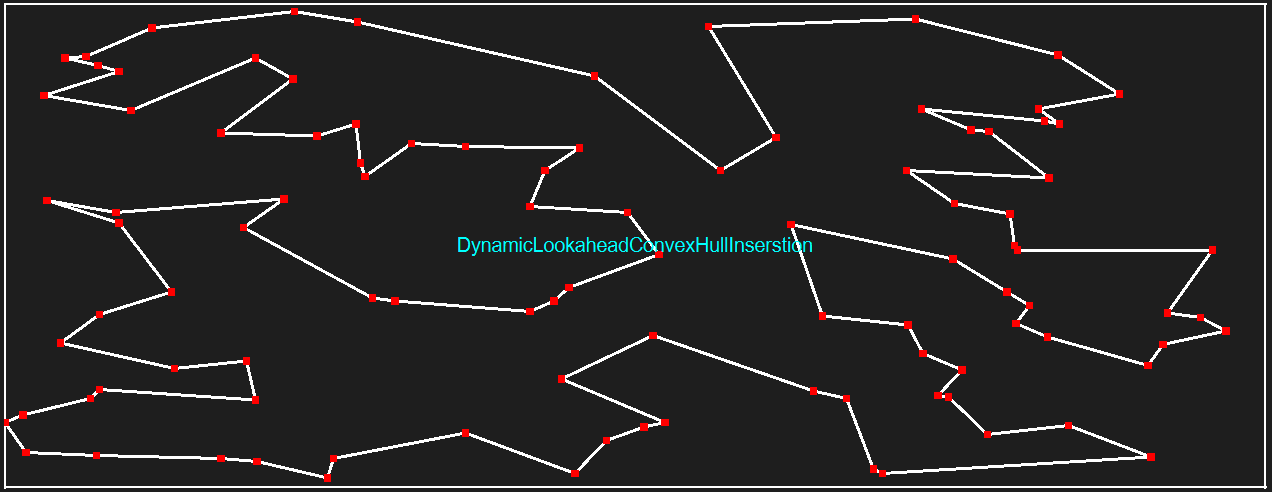
\includegraphics[width=\textwidth]{sections/image/Front_page.png} \\
    \vspace{2cm}
    
    % Author section
    \normalsize
    \textbf{Author:} Andrew Foot, 2177545 \\ [0.5cm]
    \textbf{Supervised By:} Dr Rajesh Chitnis \\ [0.5cm]
    Department of Computer Science \\
    University of Birmingham \\ [2cm]
    \textbf{Word Count:} 13,731 \\

    % Date (optional)
    \vfill
    {\large \the\year}
\end{titlepage}

\newpage
\setcounter{page}{2}  % Since title page was page 1, next is page 2

% ----------------- Abstract ----------------- %

\begin{abstract}
    The Travelling Salesman Problem(TSP) is one of the most well-known optimisation problems in graph theory due to its straightforward formulation and wide range of real-world applications. However, as an NP-Hard problem, finding exact solutions is computationally infeasible for large instances, leading to the development of various heuristics that provide sub-optimal, but practical solutions.

This report examines and implements the enhancement of look-ahead mechanisms to the Cheapest Insertion Heuristic(CIH) to create two new algorithms, balancing computational efficiency with improved solution quality for the Symmetric Travelling Salesman Problem(STSP). To achieve this, in-depth research and computational testing with the aid of a substantial software engineering project are presented in this report.

When designing a new algorithm, the theory looks at the problem needing to be solved, new issues that get introduced, and its time complexity. At the same time, software engineering looks at implementing the design and making logical improvements to decrease the time complexity. Both are vital components covered in this report. 

Evaluating any new algorithm requires a solid methodology and rigorous testing of itself and its performance against others in its class. Software has been designed and developed for empirical testing, visual inspection, and data analysis to impartially conclude the results of a new Look-Ahead Cheapest Insertion Heuristic.
\end{abstract}

\pagebreak
\tableofcontents
\pagebreak

% ----------------- Main Content ----------------- %
\begin{center}
\section{Introduction}
\end{center}

The Travelling Salesman Problem(TSP) is one of mathematics' most studied optimisation problems due to its simple problem definition and wide use case\cite{Flood1956}. The goal is to find the shortest route that visits every node exactly once. It is used in many fields and industries, as its graphing properties can be applied to various problems, leading to significant interest from both theorists and practitioners.

\begin{figure}[!ht]
    \centering
    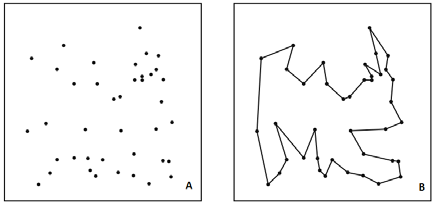
\includegraphics[width=0.9\textwidth]{sections/image/tsp.png}
    \caption{TSP And Solution}
    \cite{tsp-image}
\end{figure}

However, due to the NP-Hardness property of the problem\cite{TSP-NP-hard}, an exact solution can be computationally infeasible. Therefore, approximations are a suitable replacement for some applications where an exact solution is not required. These algorithms are called heuristics due to their approximating solutions and quick results.

Look-ahead(LA) algorithms are an algorithm design type with no formal definition. They are not a new concept, as they are primarily found in decision problems, but range from backtracking to forward checking to combinatorial search.

This report defines look-ahead as a sub-procedure that recursively checks how a greedy prediction affects future options and applies a semi-intelligent outcome with foresight. Applying foresight to avoid the common pitfalls of greedy algorithms introduces its own challenges because a look-ahead heuristic is still classified as a greedy approach; under the wrong circumstances, it will produce suboptimal results.

Dynamic look-ahead is an extension to the look-ahead algorithm design that will be explored to help resolve and improve the issues facing a standard approach to look-ahead. It aims to achieve this by changing the look-ahead search depth dynamically at runtime based on the problem at large through various metrics.

This project will apply these algorithmic designs to the existing Cheapest Insertion Heuristic(CIH) greedy algorithm to create two new algorithms, Static Look-Ahead Cheapest Insertion Heuristic and Dynamic Look-Ahead Cheapest Insertion Heuristic. Its unique design, implementation, and performance are compared to other classical algorithms and then evaluated.

An in-depth review of the Travelling Salesman Problem, existing solutions, and software optimisation techniques is conducted for the project to consider. This report researches the logical steps required to apply a look-ahead design to CIH and the potential benefits and issues that come with a look-ahead design. A scientific methodology is devised for an organised approach to the testing, evaluation, and conclusion of the findings of this project.

A significant software development project is included to verify and empirically test theoretical ideas. State-of-the-art methods and techniques are employed to ensure unbiased results and optimal performance. Algorithmic designs are coded with accuracy and are deterministic for reliability and scrutiny of the results. The same core library code is used to execute multiple runtime solutions to fit the various needs of the project. 

When evaluating a new algorithm, multiple methodologies are explored. Empirical testing on new randomly generated problems is conducted against existing conventional greedy heuristics, and then data analysis is applied. A famous testing library, TSPLib\cite{TSPLib}, of optimally solved problems serves as a ground truth to measure how the new designs perform against exact solutions.

Graphs and renders of solutions have been developed for verification and visual evidence. Allowing for easy comparison between solutions and quick data analysis is vital for later evaluations. Data collection and processing for statistics and scientific research are embedded in the analysis of each solution.

White box unit testing covered the codebase from bugs and unexpected behaviour changes. Waterfall project management helped ensure the project stayed on track and reduced the amount of refactoring and backtracking.

\subsection{Motivation}

This report will research, design, test, and evaluate the use of a look-ahead design on an existing greedy heuristic to create an improved solution over that of its greedy heuristic counterpart. This report will not attempt to solve the Travelling Salesman Problem or discuss the possibility of the P versus NP problem.

\subsection{Aims}
\label{sec:aims}

This report aims to tackle the challenges present when creating a new algorithm and to follow current research in methodology to produce a worthwhile and fair conclusion. Following this, some aims have been outlined, and each will be independently evaluated at the end of this report in Section\ref{conc:aims}.

\begin{enumerate}
  \item Design a new look-ahead algorithm that runs in polynomial time based on the greedy Cheapest Insertion Heuristic
  \item Fairly and objectively test and evaluate each performance metric of a heuristic algorithm
  \item Develop and maintain a working code base to run various algorithms reliably through a standard API
\end{enumerate}
\begin{center}
\section{Legal, Social, Ethical, and Professional Issues}
\end{center}

The British Computer Society(BCS) Code of Conduct\cite{BCSCodeOfConduct} outlines the legal, social, ethical, and professional issues in the fields of computer science and information technology. This project complies with all the conducts stated by BCS and does not produce any issues.

\begin{itemize}
    \item Public Interest:
    \begin{itemize}
    \item The research is only intended to benefit the public
    \end{itemize}
    
    \item Professional Competence and Integrity:
    \begin{itemize}
    \item This work is solely my own, and all third-party libraries used comply with their respective licensing agreements
    \item Due Diligence has been conducted into the current field research
    \end{itemize}
    
    \item Duty to Relevant Authority:
    \begin{itemize}
    \item The data and information shared in this report are faithful for all relevant authorities to read
    \end{itemize}
    
    \item Duty to the Profession:
    \begin{itemize}
    \item Throughout the project, communication with my supervisor, Dr Rajesh Chitnis, has been professional and respectful
    \end{itemize}
    
\end{itemize}
\begin{center}
\section{Literature Review: Travelling Salesman Problem} \label{lit}
\end{center}

The Travelling Salesman Problem(TSP) is two problems in graph theory: a decision and an optimisation problem\cite{Cook1971}. However, it is most famous for its optimisation version, which is what this report covers. The most basic version of the optimisation problem is finding the shortest Hamiltonian cycle from a set of nodes(vertices) with non-negative weighted edges(links) to every other node(complete graph)\cite{Flood1956}. This can be formalised in graph theory with ordered pairs \(G = (V, E)\)\cite{Dantzig1954}.

\begin{itemize}
  \item \(G\), a graph
  \item \(V\), a set of nodes
  \item \(E\subseteq \{\{x,y,w\}\ |\ x,y\in V, w\in \mathbb{R}_{\geq0},  x \neq y\}\), a list of weighted edges from node x to node y
  \label{graph_data}
\end{itemize}

\begin{figure}[!ht]
    \centering
    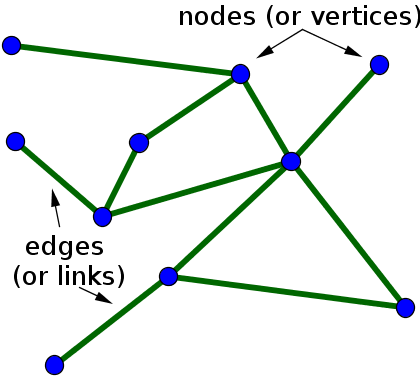
\includegraphics[scale=0.8]{sections/image/small_undirected_network_labeled.png}
    \caption{Graph Theory Diagram}
    \cite{Graph-Theory-Image}
\end{figure}


A Hamiltonian cycle is defined as from a graph, \(G =(V, E)\), an ordered list of edges creating a continuous path where every node is visited exactly once\cite{biggs1986graph}. In the research for TSP, the route can be defined as a 2-dimensional adjacency matrix, $A_{ij}$, of boolean values to represent if an edge is present in the cycle\cite{Croes1958}; It can also be listed as an ordered list\cite{Michael1970}, $P_i$,  where \(P\subseteq E\). The cost function of the cycle and the Travelling Salesman Problem is the summation of all the weights of the edges in the list \(P\) and is what is trying to be minimised\cite{Flood1956}:

\begin{equation}
    \min_{i \in P}(\sum \text{weight(}P_i))
    \label{TSPcost}
\end{equation}

Hamiltonian cycle has some formal constraints in graph theory\cite{biggs1986graph}:

\begin{itemize}
  \item \(|V| \geq 3\), There must be at least three nodes to create a cycle
  \item \(|P| = |V|\), The list must have as many edges as there are nodes in the graph
  \item \(\forall P_i: y_{i} = x_{i+1} \), Each edge in the list must create a continuous path
  \item \(\forall P_i \forall P_j:\ i\neq j, \ x_i \neq x_j, \ y_i \neq y_j\), Each node can only have two edges connecting to it in the route
\end{itemize}

\begin{figure}[H]
    \centering
    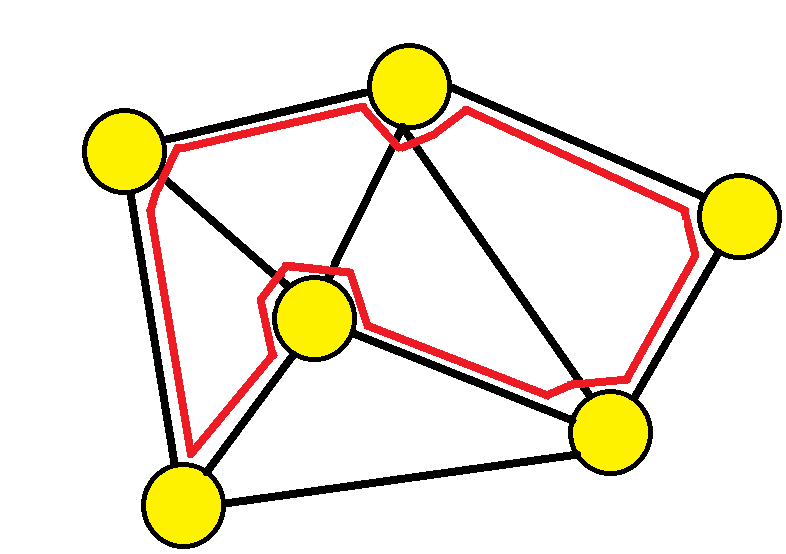
\includegraphics[scale=0.4]{sections/image/Hamiltonian.png}
    \caption{Hamiltonian Cycle}
    \cite{Hamiltonian-Path-Image}
\end{figure}

\label{hamiltonian-data}
While the adjacency matrix is more common in research, an ordered list is more memory efficient when programmatically storing a route. The list can store a list of edges or the order in which the nodes are visited. The latter is more popular as it is more memory efficient, but has slower read times. This is possible because the graph must be fully connected, therefore, the taken edges can be deduced from the adjacency matrix(Figure\ref{fig:adj}).

\begin{figure}[H]
    \centering
    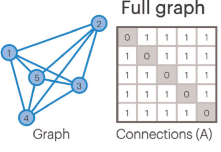
\includegraphics[scale=0.8]{sections/image/509624_1_En_15_Fig2_HTML.png}
    \caption{Adjacency Matrix}
    \label{fig:adj}
    \cite{Adjanceny-matrix-diagram}
\end{figure}

%\subsection{Versions Of Travelling Salesman Problem}
Over the years, constraints and variants of the classic optimisation problem have been conjured to fit the specific needs of researchers. Most are derived from changes to the type of graph the problem is solving\cite{Variants-tsp}: symmetric, asymmetric, Euclidean, Manhattan, two dimensions, three dimensions, and many more. But there are also new constraints like Dubins TSP\cite{Dubins-tsp}, which specifies that the route has a minimum turning radius, or K-TSP\cite{jiang2019algorithmsadaptivitygapsstochastic}, which introduces a starting hub and $k$ number of salesman/routes, or TSP with Time Windows(TSPTW)\cite{LOPEZIBANEZ20133806}, which adds temporal constraints to the problem.

\begin{figure}[!ht]
    \centering
    \begin{minipage}{0.45\textwidth}
        \centering
        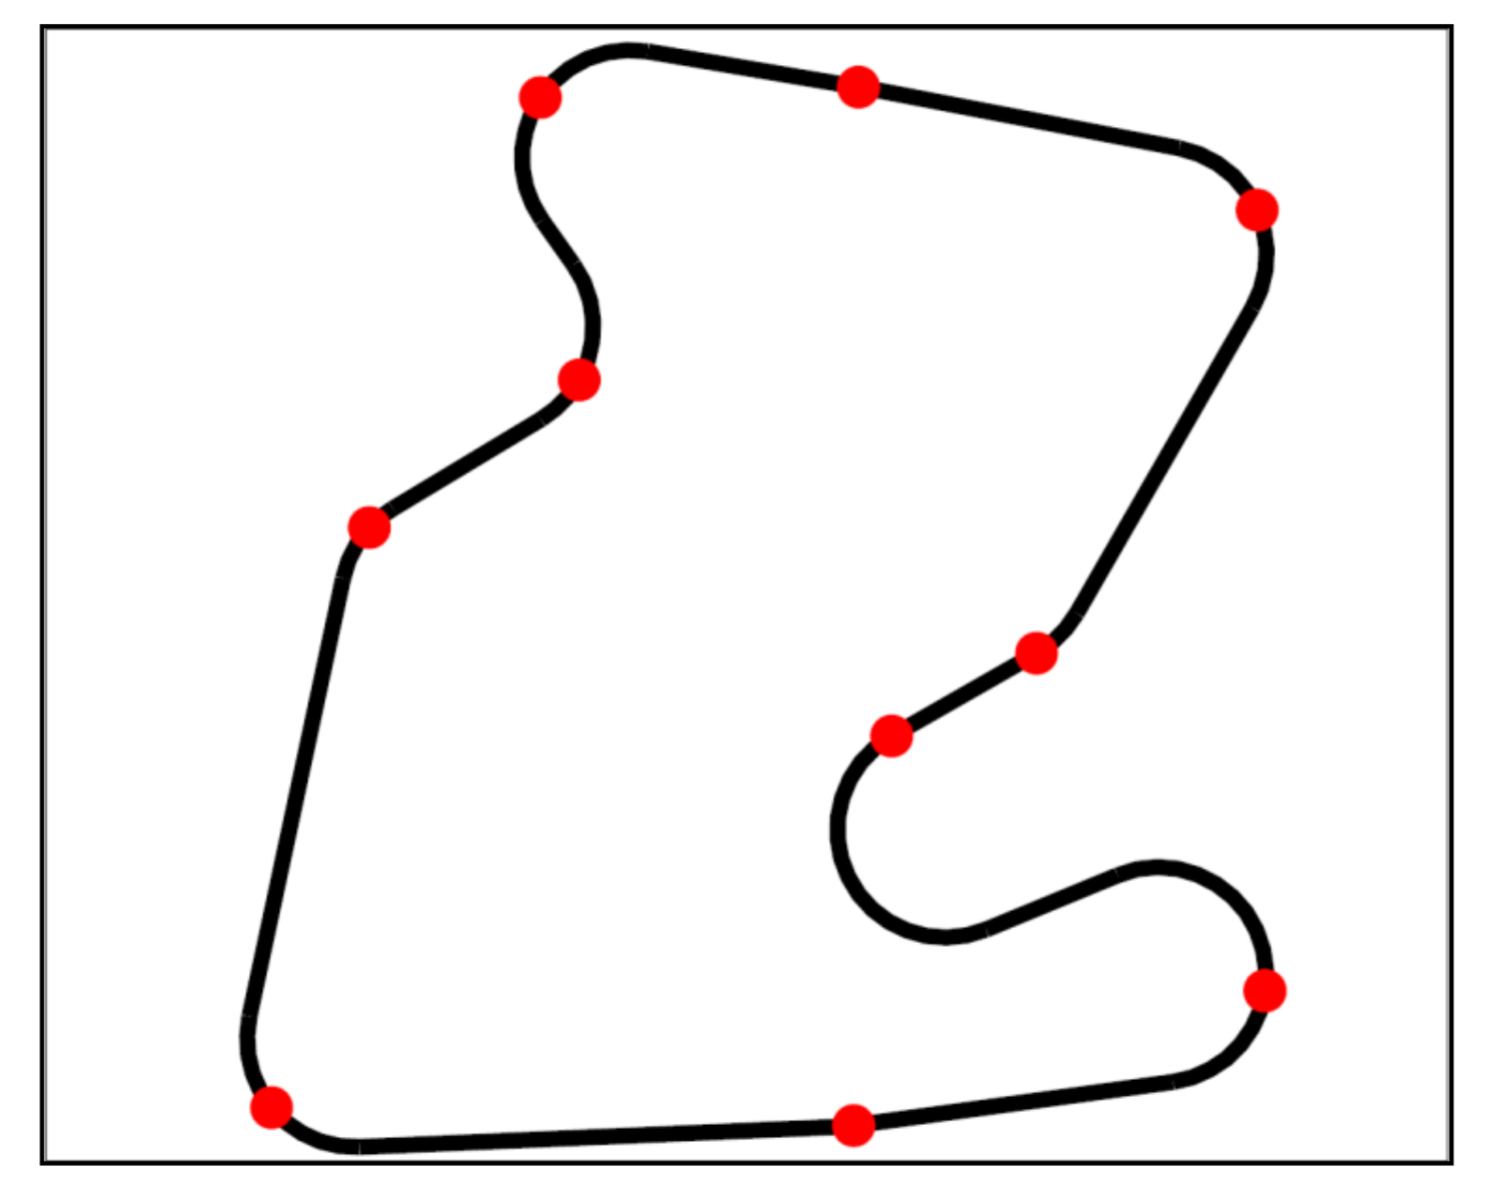
\includegraphics[width=0.9\textwidth]{sections/image/dtsp.png}
        \caption{Dubins TSP}
        \cite{dubins-tsp-picture}
    \end{minipage}\hfill
    \begin{minipage}{0.45\textwidth}
        \centering
        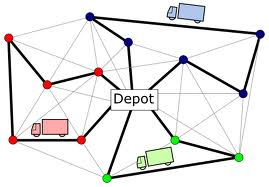
\includegraphics[width=0.9\textwidth]{sections/image/k-tsp.jpeg} % second figure itself
        \caption{K-TSP}
        \cite{K-tsp-picture}
    \end{minipage}
\end{figure}

A popular version is the symmetric two-dimensional Euclidean Hamiltonian Travelling Salesman Problem, which is used for the project for its adaptability to other problems. This is the most basic version and can be a catalyst for many other problems. It can be broken down into:
\begin{itemize}
  \item Edges between two nodes that have the same weight bidirectionally
  \item Nodes are positioned on a two-dimensional plane
  \item The distance between nodes is calculated using a straight distance
  \item The route is made up of only one Hamiltonian cycle
\end{itemize}

The TSP optimisation problem belongs to the NP-Hard classification of problems\cite{TSP-NP-hard}, as no algorithm exists for creating or verifying a solution in polynomial time. This is verifiable because there is a polynomial time reduction from the Hamiltonian cycle problem to the Travelling Salesman Problem\cite{CARMESIN2023102156}. All variants of TSP are also NP-Hard, as a polynomial-time reduction exists to handle the additional constraints\cite{Dubins-np-hard}.

When developing routes from nothing, two sub-procedures are used to generate a TSP solution. The different procedure determines if the algorithm is a tour constructor, a tour optimiser algorithm, or both\cite{Christian-tsp}. Tour constructor algorithms focus on adding unvisited nodes to a route in an optimal manner\cite{Rosenkrantz2009}. Tour optimiser algorithm focuses on improving an existing route by alternating the edges being taken\cite{tour-optimisation-paper}. The two sub-procedures are:
\vspace{0.5cm}
\begin{center}
    \begin{minipage}{0.8\linewidth}
        \begin{itemize}
            \item Construction: Iteratively adds an unvisited node to the route.
            \item Pairwise Exchange\cite{Englert2014}: Removing two edges from a route and reconnecting the resulting segments in an alternate way that still forms a cycle.
        \end{itemize}
        \captionof{table}{Sub-Procedures}
        \label{twosubprocedure}
    \end{minipage}
\end{center}
\vspace{0.5cm}
When geometric graphs are used, the Hamiltonian cycle has a property that the optimal solution will never have two edges that intersect each other due to the triangle inequality\cite{JEROMIN198970}. In Euclidean geometry, the triangle inequality states that the length of any two sides of a triangle is always greater than or equal to the length of the remaining side. Therefore, when a route is treated as a polygonal chain, a closed polygonal chain that does not form any triangles is strictly better than a polygonal chain that self-intersects and forms a triangle\cite{Kalmanson_1975}; this is the basic principle 2-opt is built upon.

\begin{figure}[H]
    \centering
    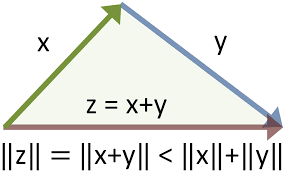
\includegraphics[scale=0.5]{sections/image/triangular_inequaility.png}
    \caption{Triangular Inequality}
    \cite{triangle-inequality-picture}
\end{figure}

\subsection{Exact Solution}
An exact or optimal solution is the route with the global minimum cost for a given graph; no other valid route has a lower cost\cite{Flood1956}. A graph can have multiple exact solutions if two or more routes have equal costs\cite{Capelli_2018}. An exact solution to the TSP is ideal in most situations, but it is sometimes a requirement in areas of research, such as DNA sequencing\cite{LEE200439}.

For a graph with \(n\) nodes, there are \(O(n!)\) possible routes\cite{Woeginger2003}. A simple approach to finding the optimal route would be a brute-force search, which calculates every possible combination of routes and stores the best result. This was taught in the year three Algorithms and Complexity module. However, with \(O(n!)\) possible routes and \(O(n)\) time to calculate the route cost, this becomes computationally infeasible after \(n\geq \approx20\)\cite{neoh2020evaluation}, due to exponential time growth\cite{Brute-Force}.

A similar mathematical problem is the sequencing problem\cite{Sequencing-problem}, which has an arbitrary cost function and a recurring scheme; this matches the TSP brute-force search. A dynamic programming solution exists for the sequencing problem\cite{DP-Sequencing} and can be applied to brute-force search\cite{TSP-DP}, which can cut down on the number of routes that need checking to \(O((n-1)2^{n-2})\)\cite{TSP-DP}. This is a significant improvement, but still means that problems after \(n\geq \approx57\) are infeasible.
\begin{figure}[H]
    \centering
    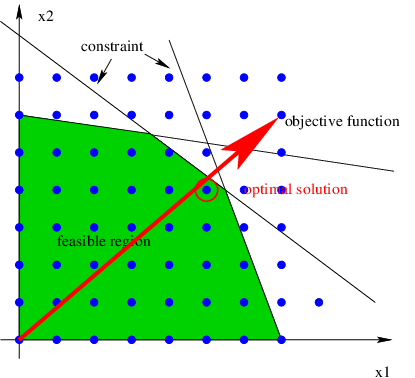
\includegraphics[scale=0.6]{sections/image/Example-Integer-Linear-Program-ILP.png}
    \caption{ILP Problem}
    \cite{ILP-diagram}
\end{figure}
Another method, not covered in the Algorithms and Complexity module, for solving exact solutions is solving TSP as an Integer Linear Programming(ILP) problem\cite{ILP}. ILP is an NP-hard optimisation problem with an objective function and a set of linear equations that must be satisfied. Some of these linear equations are developed from the definitions and constraints stated at the start of Section\ref{lit}. The worst-case time complexity for ILP is $O(n!)$\cite{diaby2006tsp}, but it can be significantly lower, depending on the problem\cite{HOOS201487}(covered in Section\ref{Concorde}).

% \begin{figure}[H]
%     \centering
%     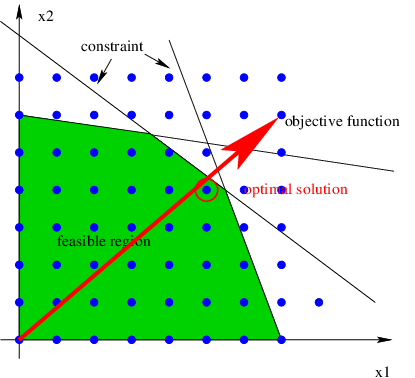
\includegraphics[scale=0.6]{sections/image/Example-Integer-Linear-Program-ILP.png}
%     \caption{ILP Problem}
%     \cite{ILP-diagram}
% \end{figure}

\subsubsection{Concorde TSP Solver}
\label{Concorde}
Due to the need for exact solutions to the Travelling Salesman Problem, research into optimising the development of exact solutions has been in development since the 1970s. William Cook, a researcher from the University of Waterloo, has made significant strides in this area over the past two decades with his team's Concorde TSP Solver\cite{concorde_tsp}, which is widely regarded as the best solver available\cite{HOOS201487}. Concorde holds the record for the largest TSP problem solved optimally at 85,900 nodes\cite{APPLEGATE200911} and is the first solver to obtain an exact solution to every problem in the TSPLib collection\cite{concorde_benchmarks}\cite{applegate2003implementing}, along with winning many awards for solving open problems\cite{amz_tsp}. It uses all of the most recent research and techniques, which this project researched and will explain.

Concorde is an extension of the University of Waterloo's research into solving Integer Linear Programming with their QSopt Linear Programming Solver\cite{APPLEGATE2007693}. Concorde solves problems by taking an existing good heuristic solution and relaxing the linear constraints to make the linear problem easier to solve\cite{applegate1998solution}. It can relax constraints using the Cutting-Plane Method, Branch-and-Bound, and Branch-and-Cut algorithms\cite{applegate2006traveling}.

\begin{figure}[H]
    \centering
    \begin{minipage}{0.45\textwidth}
        \centering
        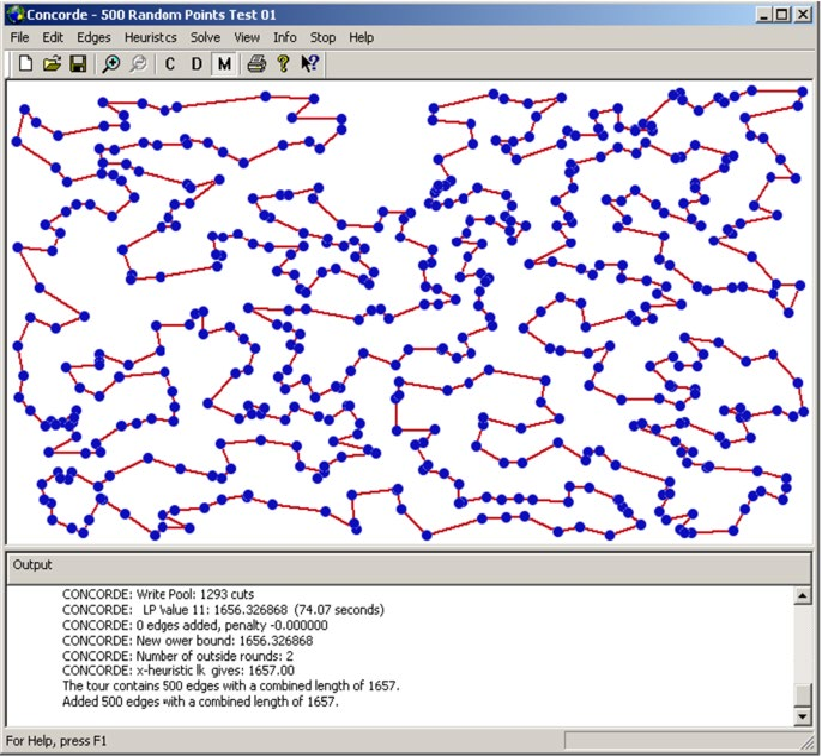
\includegraphics[width=\textwidth]{sections/image/Concorde-TSP-Solver-Solving-a-500-City-TSP-Instance.png}
        \caption{Concorde TSP Solver}
        \cite{concorde-picture}
    \end{minipage}\hfill
    \begin{minipage}{0.45\textwidth}
        \centering
        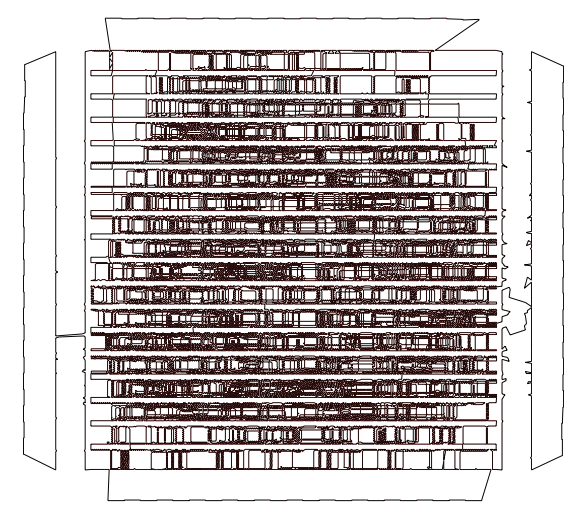
\includegraphics[width=\textwidth]{sections/image/85900_solution.png}
        \caption{85900 Node Solution}
        \cite{cook2012pursuit}
    \end{minipage}
\end{figure}

Branch-and-Bound(B\&B)(Figure\ref{fig:bab}) is an optimisation algorithm that solves Integer Linear Programming(ILP) problems by systematically branching the search space into smaller sub-problems and bounding non-promising branches\cite{MORRISON201679}. It achieves this by recursively dividing the solution space and using higher and lower bounds to eliminate sub-problems that cannot yield a better integer solution - a process known as ``pruning"\cite{VOLGENANT198283}. The best-known integer solution typically sets the upper bound, often obtained using TSP heuristic algorithms. In contrast, the lower bound is derived from solving relaxed Linear Programming(LP), where integer constraints are temporarily ignored\cite{APPLEGATE2007693}. This relaxed LP provides a bound that helps determine whether a branch should be explored further or pruned.

\begin{figure}[!ht]
    \centering
    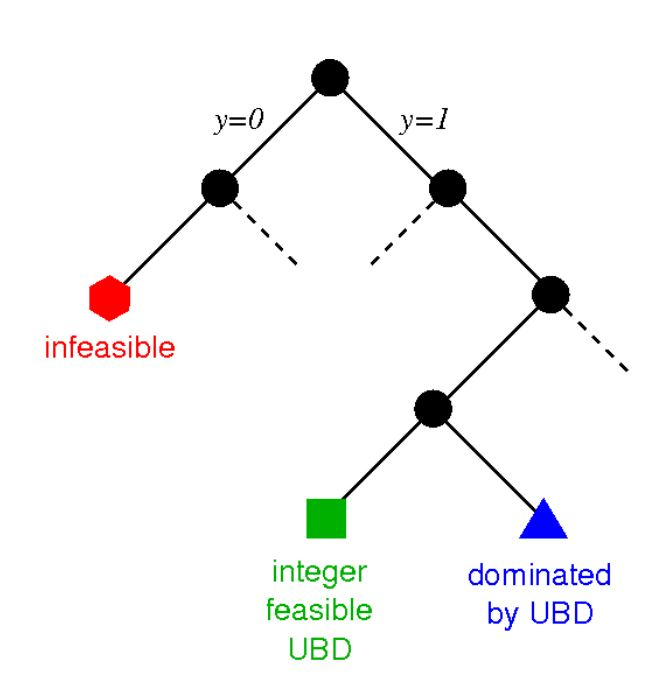
\includegraphics[width=0.5\textwidth]{sections/image/b&b.jpg}
    \caption{Branch And Bound}
    \label{fig:bab}
    \cite{cornell_bb_minlp}
\end{figure}


The Cutting-Plane Method(Figure\ref{fig:cutting}) is a technique for solving a Mixed-Integer Linear Program(MILP) by iteratively solving its Linear Programming(LP) relaxation and adding constraints(cuts) until an integer solution is found\cite{Cutting-plane}. First, it relaxes the problem to non-integer constraints and is solved as Linear Programming\cite{FLEISCHMANN1985307}. If the solution contains non-integer values, new hyperplanes(cuts) are added iteratively to the constraints until an integer solution is found\cite{applegate2003implementing}. The benefit of this approach is that LP is more straightforward to solve than MILP, but finding substantial cuts iteratively can be computationally expensive\cite{applegate2003implementing}.

\begin{figure}[H]
    \centering
    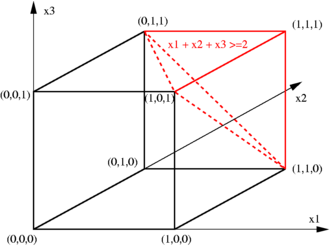
\includegraphics[width=0.6\textwidth]{sections/image/TSP_cutting_plane.png}
    \caption{Cutting-Plane Method}
    \cite{wikipedia_cutting_plane}
    \label{fig:cutting}
\end{figure}

Branch-and-Cut combines(Figure\ref{fig:bac}) Branch-and-Bound and Cutting-Plane methods into one\cite{mitchell2002branch}. It relaxes the problem to linear programming constraints, and in the pruning of Branch-and-Bound, it adds cuts back into the constraints. Added cuts can be global(cuts valid across the entire problem) or local(specific to a sub-problem in the search tree), and multiple branching strategies can be applied due to the relaxation\cite{branch-and-cut}. The benefit of Branch-and-Cut is its scalability for large-scale problems(\(n\geq\approx1000\))\cite{lu2022solvingclusteredtravelingsalesman}, making it the go-to approach for solving ILP.

\begin{figure}[H]
    \centering
    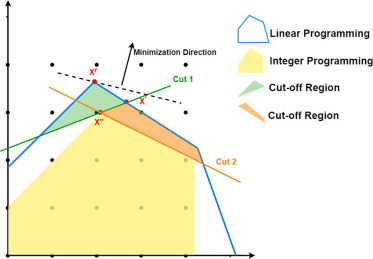
\includegraphics[width=0.6\textwidth]{sections/image/b&c.jpg}
    \caption{Branch And Cut}
    \label{fig:bac}
    \cite{ZHANG2023205}
\end{figure}

For Concorde TSP Solver, the efficiency is directly related to the starting solution provided, as it acts as the upper bound for Branch-and-Bound\cite{applegate2003implementing}. A tighter upper bound will reduce the number of valid branches by pruning more sub-problems. Therefore, research is still being applied to finding high-quality heuristics for the knock-on effect of finding a quicker exact solution in the Concorde TSP Solver.



Concorde's time complexity is not fixed because it depends on several factors, such as the starting heuristic solution and the specific instance of the problem\cite{applegate1998solution}. The worst-case complexity for branch-and-cut is exponential, \(O(2^n)\) \cite{John1963}, but practical performance is often significantly better, with standard hardware able to achieve \(n\geq\approx1000\) \cite{applegate2006traveling}. However, many software engineering optimisations are applied to hasten the solution time, allowing massive problems to be solved on supercomputers.

\subsection{Greedy Tour Construction Heuristic}

Sometimes, an approximate solution to the TSP is adequate for users when time complexity or computational resource constraints are a concern\cite{desale2015heuristic}. Amazon delivers approximately 1.6 million packages daily, with the average driver making 180 stops on their shift. This poses a logistical problem when a package could be out for delivery within a shorter time frame than the time to produce an exact solution. Another case is that many real-time path-finding applications must decide within seconds and are often limited by embedded hardware. Therefore, reliance on approximations for quick but quality solutions is still desirable for specific applications.

Heuristics are problem-solving strategies that use educated guesses to find approximate solutions quickly\cite{kokash2005introduction}. Heuristics are algorithms that follow structured logical steps; however, these logical steps take shortcuts, often trading completeness for speed. Greedy algorithms are a type of heuristic that makes local optimal choices to approximate global optimal solutions\cite{Jungnickel2013}; they are susceptible to pitfalls that cannot be solved later\cite{BANGJENSEN2004121}.

For the Travelling Salesman Problem, developing a route from a problem requires a construction strategy; these strategies are called tour constructions\cite{Christian-tsp}. A tour can be constructed in many ways and produce different results based on the starting location and variables. It usually starts with an empty route and randomly selects a node as the starting location; however, more innovative beginnings are available\cite{Christian-tsp}. Most tour constructors will iteratively add one node that is not already in the route to the route at the `head' or anywhere along the route.

Greedy tour constructors typically have polynomial time complexity and a fixed time complexity due to their exhaustive searching characteristics. Further improvements, such as caching and partitioning, can expedite the runtime, but the time complexity will remain the same. There are no guarantees on the lower bound of the solution cost against the optimal solution\cite{Vazirani2001}, as we would need to solve the P versus NP problem\cite{Vazirani2001}, which remains unproven.

\subsubsection{Nearest Neighbour}

The Nearest Neighbour Search(NNS) greedy algorithm is one of the oldest and most straightforward approaches for approximating the TSP. It was taught in the Algorithms and Complexity module. The origin of the heuristic is uncertain, but due to its simple nature, its approach is the most logical when thinking of a new method. The steps for the algorithm are as follows\cite{Nearest-neighbour}\cite{Rosenkrantz2009}:

\begin{legal}
  \item Select a random node as head and add it to the list of visited nodes
  \item Check every unvisited node:
  \begin{legal}
      \item select the unvisited node that has the lowest cost to the head
  \end{legal}
  \item Make the selected node the new head and add it to the list of visited nodes
  \item Repeat step 2 until there are no unvisited nodes
  \item Close the cycle by adding an edge from the current head to the starting node
\end{legal}

The time complexity for nearest neighbour is \(O(n^2)\)\cite{Christian-tsp}. It does \(n-1\) iterations from step 2 to step 4, and each iteration checks \(O(n)\) nodes as a possible shortest addition.

\subsubsection{Cheapest Insertion Heuristic}
\label{CIH}
The Cheapest(sometimes called shortest) Insertion Heuristic(CIH) takes a slightly more logical approach to constructing tours and was researched for this project. The addition of nodes to the route, can be added anywhere into the route\cite{Rosenkrantz2009}. The insertion cost formula for CIH calculates the breaking of the current route edge and the addition of two new edges. As nodes are added anywhere into the route, the starting route does not just have to be a single node; more advanced setups, such as Convex Hull\cite{Christian-tsp} or Shrinking Blob\cite{Jones2014}, can be adopted to improve the result\cite{jones2013computationtravellingsalesmanproblem}.

The insertion cost formula, where \(d(a,b)\) is the cost of the edge between node $a$ and $b$, \(x\) is the node to be added and \(a,b\) are consecutive nodes already in the route\cite{Rosenkrantz2009}:

\begin{equation}
    \text{Cost}(x,a,b) = d(x,a) + d(x,b) - d(a,b)  
    \label{CIH_Cost}
\cite{CIH}
\end{equation}

The steps for the algorithms are as follows\cite{CIH}\cite{Rosenkrantz2009}:

\begin{legal}
  \item Generate a starting route(random node or convex hull)
  \item For each unvisited node,
    \begin{legal}
        \item For every position in the route
        \begin{legal}
            \item Calculate the cost function of adding the node to the route position
        \end{legal}
    \end{legal}
  \item Add the selected node in the position with the lowest cost function
  \item Repeat step 2 until there are no unvisited nodes
\end{legal}

The time complexity for the cheapest insertion is \(O(n^3)\)\cite{Christian-tsp}. Its run-time changes based on the size of the starting route, but at worst, \(n-1\) iterations are run from steps 2 to 4. Each iteration is \(O(n^2)\), as \(O(n)\) unvisited nodes must calculate the cost function against \(O(n)\) positions in the route. Also, calculating the cost function(Equation\ref{CIH_Cost}) is three times more expensive than the Nearest Neighbour cost function, making CIH a significantly slower algorithm. 

\subsubsection{Convex Hull}

Convex Hull is a tour construction algorithm that does not guarantee a complete solution; instead, it generates part of a route\cite{MEERAN1997737}. The idea of a Convex Hull is to encapsulate all the points of a problem within a shape known as a convex hull\cite{lay1982convex}. Convex hulls utilise geometric locational properties of nodes, so only n-dimensional TSP problems based on Euclidean or Manhattan distance are suitable for using Convex Hulls\cite{MEERAN1997737}. 

\begin{figure}[!ht]
    \centering
    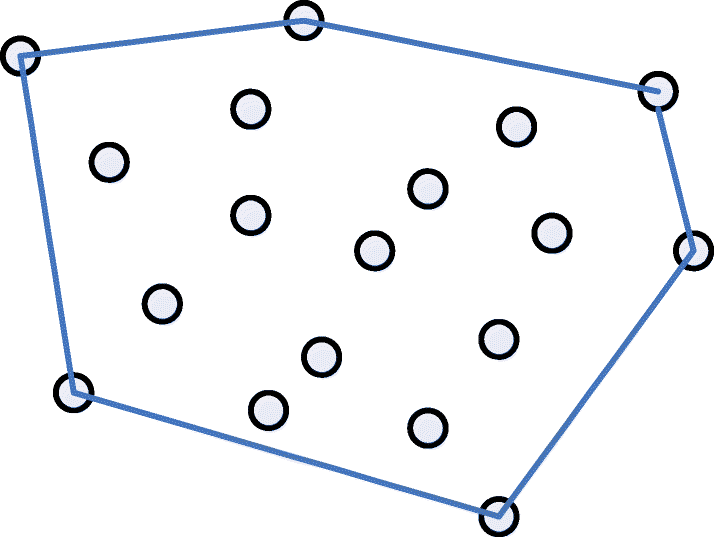
\includegraphics[width=0.4\textwidth]{sections/image/Convexhull.png}
    \caption{Convex Hull}
    \cite{Convexhull-picture}
\end{figure}


There are many algorithms for generating the structure, like Gift wrapping\cite{borgwardt1997average}, Graham scan\cite{GRAHAM1972132}, and Chan's Algorithm\cite{Chan1996}. Gift wrapping is the simplest to understand but the least efficient; the steps are\cite{borgwardt1997average}:

\begin{legal}
  \item Find the northernmost point, add it to the route, and make it the head
  \item For every node not in the route calculate the gradient to the head
  \item Add the node that forms the smallest counter-clockwise turn to the route and make it the new head
  \item Repeat step 2 until the head is back to the starting node
\end{legal}

The number of iterations is not fixed per problem, so \(h\) defines how many nodes are in the convex hull; \(h\) can be any size between \(n\geq h \geq 3\). Each time \(h\) increases by one, every node needs to be compared. Therefore, the gift-wrapping algorithm has a worse time complexity of \(O(n^2)\), but there exist more complex algorithms that run in \(O(nlog(n))\)\cite{GRAHAM1972132}.

The benefit of doing a Convex Hull is that it is a strong starting point for other heuristics\cite{MEERAN1997737}. The order of the nodes in a Convex Hull is guaranteed to be in the order of the optimal solution, as any other order of the partial route would have to cross over itself. This improves the results produced and quickens other tour constructors by reducing the number of nodes that need to be added. Algorithms that use Convex Hull address it in the name by placing it in the front, e.g. Convex Hull Cheapest Insertion Heuristic(CHCIH). This is because algorithms like CHCIH perform significantly better than CIH just by changing the starting route. 

\subsection{Existing Look-Ahead Solution}
\label{Look-ahead}

Look-ahead algorithms are valuable for dealing with decision problems\cite{murthy1995lookahead}; they are prevalent in tree searching and constraint solving\cite{frost1995look}. The premise is to evaluate future outcomes before making a decision by analysing future states to guide decision-making\cite{DongLookahead}. Look-ahead algorithms are not known for their speed, as additional computation power is required to evaluate future states, but they make up for it with above-average results\cite{SARKAR19941}. Research for look-ahead in TSP focuses primarily on adapting decision problems to different versions of TSP that can leverage this research\cite{Lin1973}.

\subsubsection{Nearest Neighbour Look-Ahead}
\label{NN-Look-ahead}
A paper by the Indian Institute of Technology called ``Improving Greedy Algorithms by Lookahead-Search"\cite{SARKAR19941} researches the use of look-ahead for solving the 0/1 Knapsack problem\cite{martello1990knapsack}. It is an optimisation decision problem for finding the optimal subset of items that maximises a cost function within a given constraint. The researchers devised that the decision problem can be formulated as a tree that can be recursively traversed to a look-ahead depth of $k$ with existing greedy algorithms\cite{SARKAR19941}. A tree structure is used because if it reaches a leaf node, then a constraint has been reached, and the algorithm should return. The researchers included pseudocode that worked for any generic greedy algorithm where the problem could be displayed as a tree\cite{SARKAR19941}.

\floatname{algorithm}{Algorithm}
\renewcommand{\algorithmicrequire}{\textbf{Input:}}
\renewcommand{\algorithmicensure}{\textbf{Output:}}

\begin{algorithm}[H]
\caption{lookahead-search$(k : \text{integer}, T : \text{tree}, G : \text{greedy algorithm})$}
\begin{algorithmic}[1]
\State $n : \text{node}$
\Comment{$k$-depth lookahead search in $T$ using $G$ as the underlying greedy algorithm.}
\State $path := \emptyset$
\State $n := \text{root}(T)$
\State lookahead$(k, n, G)$
\State print $path$ as the solution
\end{algorithmic}
\cite{SARKAR19941}
\end{algorithm}

\noindent Where Procedure \textit{lookahead} is defined recursively as follows:

\bigskip

\begin{algorithm}[H]
\caption{lookahead$(k : \text{integer}, n : \text{node}, \text{Greedy} : \text{greedy algorithm})$}
\begin{algorithmic}[1]
\State $l, m : \text{node}$
\If{$n$ is a leaf node}
    \Return
\Else
    \State Get $m \in \text{des}(n, k)$ such that
    \State \(
    \text{cost}(n \rightarrow m) + \text{Greedy}(m) = \min_{l \in \text{des}_{n, k}} \left\{ \text{cost}(n \rightarrow l) + \text{Greedy}(l) \right\}
    \)
    \State $m := \text{succ}(n \rightarrow m)$
    \State $path := path + \langle n, m \rangle$ \Comment{augment path; path is global}
    \State lookahead$(k, m, \text{Greedy})$
\EndIf
\end{algorithmic}
\cite{SARKAR19941}
\end{algorithm}

The researchers applied this pseudocode to the nearest neighbour greedy algorithm because it can be easily applied to a tree structure. The head node is the root state, and the greedy algorithm can be applied recursively to generate the states of the children nodes.

The researchers found that only minor improvements were made when applying the look-ahead design, however, it can produce better results than its greedy algorithm counterpart\cite{SARKAR19941}.

\subsubsection{Dubins Look-Ahead TSP Solver}

A paper by Automation Science and Engineering, titled ``Discretization-Based and Look-Ahead Algorithms for the Dubins Traveling Salesperson Problem" \cite{Cohen2017}, investigates the use of look-ahead for solving the Dubins version of the TSP. Dubins Travelling Salesman Problem(DTSP) adds the constraint that the route has a minimum turning radius\cite{Dubins-tsp}; this is to mimic the constraint that something like a fixed-wing aircraft faces.

The researchers developed a look-ahead algorithm for DTSP, where L is the look-ahead depth\cite{Cohen2017}:

\begin{legal}
  \item Get a solution for a corresponding Euclidean TSP
  \item Selected a random node as the head, $h$, and generate an initial heading to $h+1$ 
  \item Iterate $h$ for all nodes in the solution
  \begin{legal}
    \item Brute force calculates the shortest Dubins route for the subset, $h-1$ to $h+L-2$ nodes, where the heading of $h-1$ is fixed
    \item Permanently set the heading of $h$
  \end{legal}
  \item Return the newly organised solution
\end{legal}

The look-ahead part of this algorithm involves brute-forcing a small subset of the route and setting only the heading of node $h$. $h-1$ heading has to be fixed to allow for the continuous build-up of a Dubins route. Brute forcing a subset of the problem does not result in an exact solution because faults are introduced in the combination step, but it does provide a better result than if a greedy approach were taken.

%\subsubsection{Beam Search Heuristic}

%A paper by Yuan Ze University called ``A Beam Search Heuristic for the Traveling Salesman Problem with Time Windows" researches the use of look-ahead for solving the TSP with Time Windows(TSPTW). TSPTW introduces a temporal constraint for when a node can be visited, this is found in networking problems.

%Beam Search is a modification on the breadth-first search of trees by pruning the number of nodes that are tracked at each layer to a value, $\beta$. As fewer nodes are evaluated at each layer, it saves on memory and computational power by only choosing the most potential nodes via estimations. However, the results of the pruning are dependent on how accurate the estimations are.

%The researchers proposed a few Beam Search techniques for TPSTW with Local evaluation, Global evaluation, and implementation details of the evaluation. Each uses partial routes(the beam nodes) and different ways of iteratively inserting which node. For Local Evaluation, it generates all nodes to a depth $L$ and creates a cost function(weighs route length, time weight violations).

\subsection{Tour Optimisation Heuristic}

Sometimes, the initially constructed route is not good enough, and simple improvements can be made to the route's ordering to achieve a better result \cite{Christian-tsp}. This is where Tour Optimisation algorithms are used to improve the ordering and refine the edges taken from an already complete cycle while maintaining the properties of the TSP\cite{Christian-tsp}.

Tour Optimisation heuristics effectively resolve local pitfalls that have been taken, but they struggle to find global pitfalls. Optimisers rarely find the exact solutions to a problem, but they are valuable as they often find improvements on existing solutions cheaply. This report researches its design.

\subsubsection{2-opt}

The simplest optimisation heuristic is Croes's 2-opt local search algorithm in 1958\cite{Croes1958}. It utilises the property that any two edges crossing over each other are suboptimal and calculates whether swapping edges can produce a better result. For Symmetric graphs, the cost function below calculates if swapping two edges will benefit the route:

\begin{equation}
    Cost(r_i,r_j) = d(r_i,r_j) + d(r_{i+1},r_{j+1}) -d(r_i,r_{i+1}) - d(r_j,r_{j+1})
\cite{Englert2014}
\end{equation}

The steps for 2-opt are as follows\cite{Croes1958}:

\begin{legal}
    \item For each pair of edges $(i, j)$, where $i$ ranges from $0$ to $n-1$ and $j$ ranges from $i+2$ to $n$:
    \begin{itemize}
        \item Calculate the cost of swapping the edges.
        \item If the swap results in a negative cost, perform the swap.
    \end{itemize}
    
    \item Repeat step 1 until no swaps result in a negative cost.
\end{legal}

The time complexity of 2-opt is often difficult to predict in real-world examples, as it is unknown how many iterations it will perform. Each iteration takes \(O(n^2)\)\cite{Englert2014}, as it checks two nested For loops of combinations. Although 2-opt is likely to converge after only a few iterations, the worst-case scenario is \(O(n^2)\) iterations due to the numerous combinations of swaps available for an edge before it reaches a location it has been in before. Therefore, the worst case for 2-opt is \(O(n^4)\)\cite{Englert2014}, however if applying a limit of $m$ iterations results in \(O(m\cdot n^2)\). 

\subsection{Software Engineering Optimisation}
\label{SWEOps}
When solving the TSP, the fundamentals of each algorithm remain the same, but data structures and algorithms can be applied to achieve a constant-factor speed-up. Each software engineering optimisation benefits the computational runtime for the average case, but the Big O time complexity remains the same in the worst case\cite{applegate2006traveling}. 

\subsubsection{Caching}
\label{lit:Caching}
Caching is the process of storing computational results to be used later for quick callback. When the problem is assigned as a list of nodes, the edge weights are not necessarily known at run time\cite{applegate2006traveling}. Calculating edge weights can be expensive depending on the TSP problem type(3D Euclidean, Global Coordinates, A* Pathfinding)\cite{Caching-performance}. Therefore, a 2D Adjacency Matrix can store $n^2$ edge results. Two fill strategies can be applied to deal with caching:

\begin{itemize}
    \item Full: Calculate every edge weight before trying to solve the problem
    \item Partial: See if the edge weight has been cached before; if not, calculate the edge
\end{itemize}

If it is known that an algorithm will scan most edges, doing full caching is ideal, as there is no overhead for checking if a cache miss has occurred. If an algorithm does not scan all the edges, partial caching helps reduce unnecessarily expensive calculations.

\subsubsection{Partitioning}
\label{partitioning}
Partitioning is the process of bucketing nodes into groups based on the geometric location of the point\cite{applegate2006traveling}. There are two use cases for partitioning in the Travelling Salesman Problem\cite{karp1977probabilistic}\cite{Clustering-Tsp}\cite{Partioning-tsp}\cite{lin2022grid}:

\begin{itemize}
    \item Closeness proximity: Reduce the search size of nodes based on proximity
    \item Creating smaller problems:
        \begin{enumerate}
            \item Group sets of nodes together
            \item Solve each set
            \item Merge the solutions to solve the original problem
        \end{enumerate}
\end{itemize}

Closeness proximity is helpful when evaluating potential nodes in heuristics\cite{Partioning-tsp}; it can cheaply exclude nodes as valid options. The partitioning algorithm's search time is typically $O(log(n))$; therefore, reducing the search space usually results in an expedited solution without affecting the result.

Splitting a large problem into smaller problems can be useful as time complexity grows exponentially\cite{karp1977probabilistic} with problem size. By dividing the problem, each solution becomes more manageable, but the solution quality drops as decision boundaries are formed between the smaller problems, resulting in disjointed routing\cite{lin2022grid}. It is merging of solutions step that introduce imperfections in the solution quality\cite{tsp_subproblems}.

There are many partitioning algorithms, but the most common are K-means Clustering\cite{k-means}, Grid-based\cite{arora1998polynomial}, and Quad-Trees\cite{arora1998polynomial}.

\begin{itemize}
    \item K-means Clustering: Given $k$ clusters; distribute each cluster such that the nodes are evenly grouped between the clusters
    \item Grid-based partitioning: Split the graphing area into evenly distributed quadrilaterals and bucket the nodes to them
    \item Quad-Trees: Subdivides the graphing area into smaller and smaller quadrilaterals in a quad-tree structure; nodes are assigned at each layer of the tree
\end{itemize}

K-means clustering is expensive to calculate and progressively more complex as the number of clusters increases\cite{k-means-2}. However, many clusters are beneficial when partitioning the TSP problem, and K-means struggles when there is an even distribution of points\cite{k-means}.

\begin{figure}[H]
    \centering
    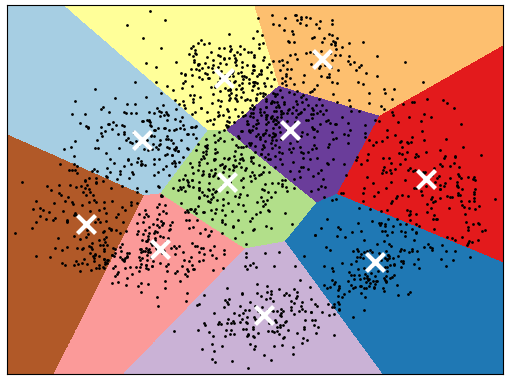
\includegraphics[width=0.65\textwidth]{sections/image/k-means.png}
    \caption{K-Means Partitioning}
    \cite{scikit-learn-kmeans-example}
\end{figure}

Grid-based partitioning is the most straightforward approach with the quickest search and creation times and works well for evenly distributed points. When the points are concentrated, grid-based partitioning fails to separate the points by grouping a large number of points in the same bucket.

\begin{figure}[H]
    \centering
    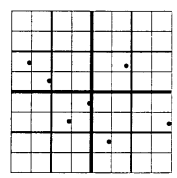
\includegraphics[width=0.4\textwidth]{sections/image/Grid-based.png}
    \caption{Grid-based Partitioning}
    \cite{arora1998polynomial}
\end{figure}


Quad-tree partitioning takes a hierarchical approach by subdividing the problem based upon the points\cite{samet1984quadtree}. As each point is assigned its own node in the tree, testing for closeness can be more precise, and the results are better for densely packed nodes\cite{arora1998polynomial}. However, the construction is expensive\cite{samet1984quadtree}, there is an overhead in search time\cite{samet1984quadtree}, and it requires a significant amount of memory.

\begin{figure}[H]
    \centering
    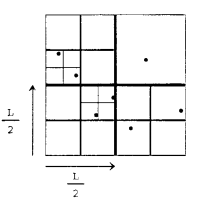
\includegraphics[width=0.4\textwidth]{sections/image/Quad-tree.png}
    \caption{Quad-Tree Partitioning}
    \cite{arora1998polynomial}
\end{figure}

\begin{table}[!ht]
\centering
\begin{tabular}{|l|l|l|l|}
\hline
\multicolumn{1}{|c|}{{ \textbf{Partitioning}}} & \multicolumn{1}{c|}{{ \textbf{Creation Time}}} & { \textbf{Read Time}} & { \textbf{Partitioning Result}} \\ \hline
K-Means                                           & O(2nki)                                           & O(1)                     & Average                                 \\ \hline
Grid-Based                                        & O(n)                                              & O(1)                     & Worst                                 \\ \hline
Quad-Tree                                         & O(nlog(n))                                        & O(log(n))                & Best                               \\ \hline
\end{tabular}
\end{table}

Although partitioning has many benefits, it requires the data to have geometric properties. The benefits are also not guaranteed, especially when the nodes are densely packed.

\subsubsection{Parallelisation}

Parallel computing involves splitting calculations across multiple processors and executing them simultaneously\cite {Parallel-computing}. There are many challenges, mainly related to data handling and synchronisation\cite{Navarro_Hitschfeld-Kahler_Mateu_2014}. But the Travelling Salesman Problem lends itself well to parallelisation due to the iterative nature of finding the best fit and only changing the problem state once all options have been considered\cite{KINDERVATER1989249}. Parallelisation is how cutting-edge technology like Concorde TSP Solver can solve massive problems using supercomputers\cite{applegate2003implementing}.

GPUs can also be applied to TSP algorithms\cite{applegate2003implementing} due to their capabilities in matrix arithmetic and vectorisation programming. Two 2D Adjacency Matrices are multiplied together, and the grand sum is taken to calculate the length of the route, allowing for quick calculations. Researchers tested the speed difference for a few algorithms and recorded a dramatic reduction in run-time of 24.2 times quicker than their CPU counterparts\cite{GPU}.
\begin{center}
\section{Research: Look-Ahead Heuristic}
\end{center}

Look-ahead(LA) has many different definitions\cite{HARALICK1980263}, but for a deterministic system, knowledge of future outcomes(states) can be determined if the current state is known; this is defined as foresight, and it can be used to evaluate options more intelligently\cite{sharma2024notelookaheadreallife}.

As mentioned in Section\ref{Look-ahead}, look-ahead algorithms and their design have already been adopted to solve the Travelling Salesman Problem and its variants. In Section\ref{NN-Look-ahead}, the greedy Nearest Neighbour Search algorithm was employed for the STSP to conform to the look-ahead algorithm proposed in their research. This is not possible for the Cheapest Insertion Heuristic.

\subsection{Problem To Solve}
\label{problem}
Greedy heuristics rarely produce global optimal solutions because they only evaluate locally optimal decisions, whereas the exact solution makes trade-offs at the local level to achieve better gains globally\cite{BANGJENSEN2004121}. These pitfalls are often hard to spot and are practically irreversible once made, especially in TSP\cite{GUTIN200281}.

% \begin{figure}[!ht]
%     \centering
%     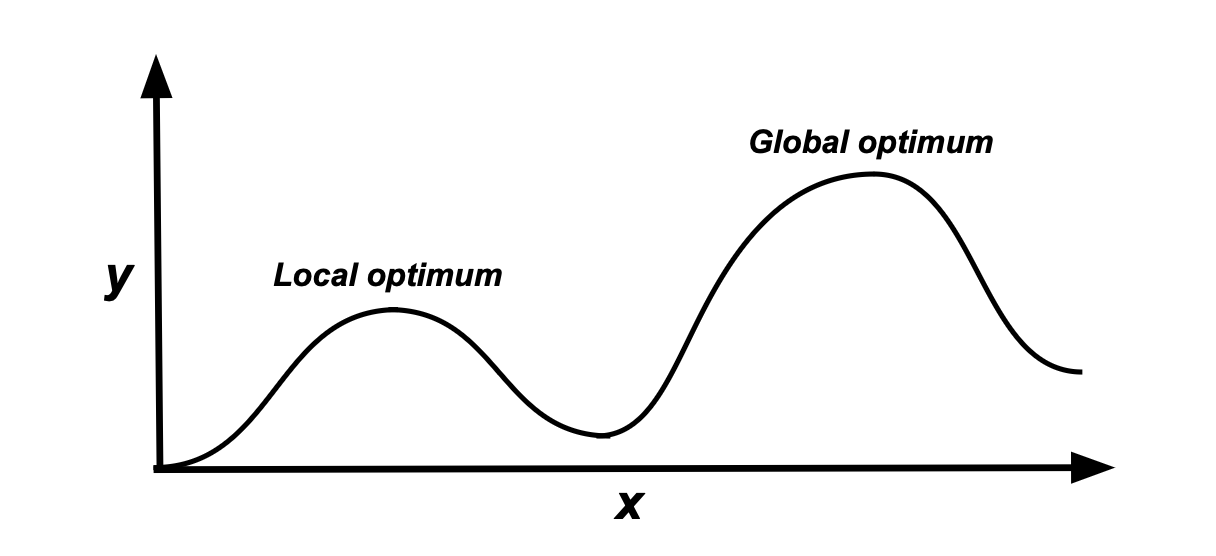
\includegraphics[width=\textwidth]{sections/image/Hill_climb.png}
%     \caption{Local Optimal vs Global Optimal Illustration}
%     \cite{hill_climbing_medium}
% \end{figure}

The cause of local optimal pitfalls varies for each algorithm, but for the CIH(Section\ref{CIH}), the pitfall occurs when a cluster is chosen because a single node is closest to the route, whereas a better cluster construction is possible in another way.

\begin{figure}[H]
    \centering
    \begin{minipage}{0.33\textwidth}
        \centering
        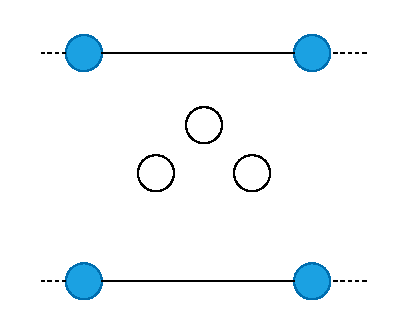
\includegraphics[page=1, width=1.2\textwidth]{sections/image/dissertationdemo.drawio.pdf}
        \caption{Base Problem}
        \label{fig:tsp_problem}
    \end{minipage}\hfill
    \begin{minipage}{0.33\textwidth}
        \centering
        \includegraphics[page=2, width=1.2\textwidth]{sections/image/dissertationdemo.drawio.pdf}
        \caption{Incorrect Solution}
        \label{fig:CIH_solution}
    \end{minipage}\hfill
    \begin{minipage}{0.33\textwidth}
        \centering
        \includegraphics[page=3, width=1.2\textwidth]{sections/image/dissertationdemo.drawio.pdf}
        \caption{Correct Solution}
        \label{fig:TSP_Optimal}
    \end{minipage}
\end{figure}


In Figure\ref{fig:tsp_problem}, the base problem involves a partial route that passes through the top and bottom of a cluster of three nodes in the centre. CIH will construct the local optimal route(Figure\ref{fig:CIH_solution}) to the cluster in the order shown in the diagram based on picking local optimal options using the cost function(Equation\ref{CIH_Cost}). This is because the topmost node is closest to the route and therefore has the lowest cost, whereas picking one of the other suboptimal nodes would result in the global optimal solution(Figure\ref{fig:TSP_Optimal}).

\subsection{Static Look-Ahead Cheapest Insertion Heuristic(SLACIH)}
\label{SLACIH}
This report explains how a look-ahead search of static depth is applied to CIH. To help avoid pitfalls, a look-ahead design can be employed to guide decision-making\cite{DongLookahead}. Applying look-ahead to the Cheapest Insertion Heuristic(CIH) cannot be done in the same manner as the Look-Ahead Nearest Neighbour\cite {SARKAR19941}(Section\ref{NN-Look-ahead}); this is due to the nearest neighbour using a sequential head as a point of insertion, while CIH evaluates every node to be added anywhere in the route.

This report examines a new algorithm, the Static Look-Ahead Cheapest Insertion Heuristic(SLACIH), or look-ahead insertion for short. If a specific look-ahead depth is specified, it can be listed in brackets after the name, e.g. SLACIH(3) for a depth of 3. 

Designing an effective and working look-ahead algorithm requires the heuristic to create a wide variation in branching solutions, enabling efficient foresight to be achieved. Taking the intuitive approach of doing sequential CIH iterations will not be effective. This is because the probability of finding unique and relevant solutions is low, given that the CIH iterations are unrelated to past insertions. To solve this, a temporary path which contains only past insertions is used exclusively as the search space for evaluating CIH in the look-ahead. This divides the SLACIH search into two subprocesses:

\begin{itemize}
    \item Normal CIH search to find where it would be added to the partial path
    \item Temporary look-ahead search to find which nodes would be added next based on previous insertions
\end{itemize}

This preserves the properties of the CIH cost function(Equation\ref{CIH_Cost}), allowing nodes to be added anywhere in the route, provided that the look-ahead only considers options that are relevant. The steps of SLACIH are as follows:

\begin{legal}
    \item Generate an initial starting partial set \label{LAI_Init}
    \item For each unvisited node:  \label{LAI_For1}
    \begin{legal}
            \item Calculate the cost function of adding the node to every position in the partial route \label{LAI_CIH}
            \item Add the unvisited node and the two visited nodes found in 2.1 to a temporary route \label{LAI_CIH2}
            \item Set a new depth limit if the depth exceeds the number of unvisited nodes \label{LAI_CIH3}
            \item For each unvisited node:\label{LAI_For2}
            \begin{legal}
                \item Calculate the cost function of adding the node to every position in the temporary route\label{LAI}
                \item Add the cheapest node to the temporary\label{LAI2}
                \item Increases depth count by one \label{LAI3}
                \item Repeat step 2.4 until the desired look-ahead depth \label{LAI4}
            \end{legal}
    \end{legal}
    \item Calculate the temporary route length and compare against best known \label{LAI_Calc}
    \item Add the original node to the position found in step 2 \label{LAI_ADD}
    \item Repeat step 2 until there are no unvisited nodes \label{LAI_While}
\end{legal}

When comparing it to CIH, steps 1, 2.1, 4, and 5 are identical to those in CIH, with steps 2.2 to 3 forming part of the look-ahead design. The look-ahead design considers every node, $n$, against a partial route of size $depth+2$, for $depth$ iterations. Counting the nested For loops, the time complexity can be calculated:

\begin{equation}
O(\tcboxmath[boxmath={blue}{CIH}]{n^2 \cdot (n}+\tcboxmath[boxmath={red}{LA}]{n\cdot (\text{depth}+2)\cdot \text{depth}}))
\label{equ:statictime}
\end{equation}

\begin{tikzpicture}[remember picture, overlay, font=\sffamily]
\draw[blue,->] (CIH.north) --++(120:5mm) node[anchor=south]{CIH};
\draw[red,->] (LA.north) --++(70:5mm) node[anchor=south]{Look-ahead};
\draw[decorate, decoration={brace, mirror, raise=3pt, amplitude=2mm}] (CIH.south west)--(LA.south east) node[below=3mm, midway]{SLACHI Time Complexity};
\end{tikzpicture}

But can be simplified to $O(n^5)$:
\begin{gather*}
\begin{aligned}
    O(n^2 \cdot (n+n\cdot (\text{depth}+2) \cdot \text{depth})) & \quad \text{// Base equation} \\ 
    O(n^2 \cdot (n+n\cdot \text{depth}^2)) & \quad \text{// Simplify and ignore +2} \\ 
    O(n^3 + n^3\cdot \text{depth}^2) & \quad \text{// Expand brackets} \\ 
    O(n^3 + n^3\cdot n^2) & \quad \text{// Worse-case value of depth} \\
    O(n^3 +n^5) & \quad \text{// Simplify} \\ 
    O(n^5) & \quad \text{// Ignore lower-order terms}
\end{aligned}
\end{gather*}
Look-ahead depth can have values $n\geq\text{depth}\geq0$, allowing it to be applied to $n$ in Big O notation. It also shows that the time complexity is bound to a quintic polynomial(5th power), regardless of the depth of the look-ahead.

Visually, the logic of evaluating temporary routes can be illustrated in geometric cases for each iteration. Blue nodes represent visited nodes, white nodes represent unvisited nodes, the orange node represents the node being considered, and yellow lines and nodes represent the temporary route.

\begin{center}
    \textbf{Inner Working}
\end{center}

\begin{figure}[!ht]
    \centering
    \begin{minipage}{0.33\textwidth}
        \centering
        \includegraphics[page=8, width=1.2\textwidth]{sections/image/dissertationdemo.drawio.pdf}
        \caption{Node 1}
        \label{node1}
    \end{minipage}\hfill
    \begin{minipage}{0.33\textwidth}
        \centering
        \includegraphics[page=9, width=1.2\textwidth]{sections/image/dissertationdemo.drawio.pdf}
        \caption{Node 2}
    \end{minipage}\hfill
    \begin{minipage}{0.33\textwidth}
        \centering
       \includegraphics[page=10, width=1.2\textwidth]{sections/image/dissertationdemo.drawio.pdf}
        \caption{Node 3}
        \label{Node3}
    \end{minipage}
\end{figure}

Figures\ref{node1}-\ref{Node3} show SLACIH(1) with a look-ahead depth of one, evaluating each unvisited node with foresight in yellow. Unlike CIH(Figure\ref{fig:CIH_solution}), which incorrectly considers the northernmost node due to its close proximity to the route, SLACIH calculates the cost of adding the node and the next.


\begin{center}
    \textbf{Outer Working}
\end{center}

\begin{figure}[H]
    \centering
    \begin{minipage}{0.33\textwidth}
        \centering
        \includegraphics[page=4, width=1.2\textwidth]{sections/image/dissertationdemo.drawio.pdf}
        \caption{Iteration 1}
        \label{Itt1}
    \end{minipage}
    \begin{minipage}{0.33\textwidth}
        \centering
        \includegraphics[page=5, width=1.2\textwidth]{sections/image/dissertationdemo.drawio.pdf}
        \caption{Iteration 2}
    \end{minipage}
\end{figure}
\begin{figure}[!ht]
    \centering
    \begin{minipage}{0.33\textwidth}
        \centering
        \includegraphics[page=6, width=1.2\textwidth]{sections/image/dissertationdemo.drawio.pdf}
        \caption{Iteration 3}
        \label{Itt3}
    \end{minipage}
    \begin{minipage}{0.33\textwidth}
        \centering
        \includegraphics[page=7, width=1.2\textwidth]{sections/image/dissertationdemo.drawio.pdf}
        \caption{Solution}
        \label{Itt4}
    \end{minipage}
\end{figure}

Figures\ref{Itt1}-\ref{Itt4} show SLACIH(1) with a look-ahead depth of one, iteratively adding the next node to the route based on its evaluation of the cheapest temporary route found during the inner workings. In Figure\ref{Itt3}, there is no look-ahead(yellow lines) because there are no more unvisited nodes to visit. Therefore, the look-ahead depth is defined by:

\begin{equation}
    \text{depth} = \min(\text{depth}, \text{\# of unvisited nodes}) = \min(\text{depth}, |\text{graph}|-|\text{route}|-1)
\end{equation}


\pagebreak
\subsubsection{Pseudocode}

\begin{algorithm}[H]
\caption{SLACIH$(depth : \text{integer}, g: \text{Graph})$}
\begin{algorithmic}[1]
\State $path := \text{initial partial set}$ \Comment{Random node or Convex Hull(Step\ref{LAI_Init})}
\While{$\exists$ node $\notin$ path} \Comment{Step\ref{LAI_While}}
    \State $[b\_node,\ b\_position,\ b\_cost] := \text{default values}$
    \For{node $\notin$ path} \Comment{Step\ref{LAI_For1}}
        \State [node, position, cost] = CIH-Search$(depth,\ node,\ path, g)$
        \If{$cost < b\_cost$} \Comment{Step\ref{LAI_Calc}}
            \State $[b\_node,\ b\_position,\ b\_cost] = [node,\ position,\ cost]$
        \EndIf
    \EndFor
    \State path.add(b\_node, b\_position)\Comment{Step\ref{LAI_ADD}}
\EndWhile
\end{algorithmic}
\end{algorithm}

\begin{algorithm}[H]
\caption{CIH-Search$(\text{depth} : \text{integer}, n : \text{Node}, \text{path} : \text{route},g : \text{graph})$}
\begin{algorithmic}[1]
\State $[b\_position,\ b\_cost] := \text{default values}$
\For {node $\in$ path} \Comment{Step\ref{LAI_CIH}}
    \State $cost := Distance(n, node_i, node_{i+1})$
    \If{$cost < b\_cost$}
        \State$[b\_position,\ b\_cost] = [i,cost]$
    \EndIf
\EndFor


\State \\$temporary\_list := \{node_i,\ n,\ node_{i+1}\}$ \Comment{Step\ref{LAI_CIH2}}
\State $depth := \min(depth, |g|-|path|-1)$\Comment{Step\ref{LAI_CIH3}}\\

\State $b\_cost := $lookahead-search$(depth,\ temporary\_path,\ path,g)$
\State \textbf{Return} $[b\_position,\ b\_cost]$
\end{algorithmic}
\end{algorithm}

\begin{algorithm}[H]
\caption{lookahead-search$(depth : \text{integer},temporary\_path : \text{path},path : \text{path}, g : \text{graph})$}
\begin{algorithmic}[1]
\If{depth < 0}
\State Return 0
\EndIf
\State $[b\_node,\ b\_position,\ b\_cost] := \text{default values}$

\For {node $\in$ g $\ni temporary\_path, path$ } \Comment{Step\ref{LAI_For2}}
    \For{p $\in temporary\_path$}
        \State $cost := Distance(node, p_i, p_{i+1})$ \Comment{Step\ref{LAI}}
        \If{$cost < b\_cost$}
            \State$[b\_node,\ b\_position,\ b\_cost] = [node,\ i,\ cost]$
        \EndIf
    \EndFor
\EndFor

\State temporary\_path.add(b\_node, b\_position)\Comment{Step\ref{LAI2}}
\State depth = depth - 1 \Comment{Step\ref{LAI3}}
\State Return lookahead-search$(depth-1,temporary\_path, path,g)$  \Comment{Step\ref{LAI4}}
\end{algorithmic}
\end{algorithm}

\subsection{Pitfalls With New Solution}
\label{pitfall}
Pitfalls are specific cases where an algorithm makes the wrong choice; all heuristics have them, including look-ahead design. While look-ahead is valuable in identifying local pitfalls, due to the greedy nature of CIH, it is not enough to prevent it from making mistakes(Figure\ref{fig:tsp_problem}). SLACIH remains a greedy heuristic that can fail under certain circumstances, as demonstrated in Section\ref{problem}. This is due to the reliance on a cost function and local greedy optimisation remaining as the decision-making process at each iteration of the look-ahead.

This can be proven by contradiction by applying SLACIH($n$) to a problem and observing that it fails to achieve the exact solution. If SLACIH($n$) provided an exact solution for every TSP problem, then the P=NP problem would be solved because SLACIH($n$) has a polynomial time complexity of $O(n^5)$.

SLACIH introduces another pitfall unique to look-ahead algorithms. The depth of look-ahead searches can impact the decision-making process when considering the required partial route size(depth) as the cost function. This can be visualised in geometric space with a small cluster of nodes being considered by SLACIH(3), a look-ahead depth of 3.

\begin{figure}[!ht]
    \centering
    \begin{minipage}{0.45\textwidth}
        \centering
        \fbox{\includegraphics[page=12, width=0.95\textwidth]{sections/image/dissertationdemo.drawio.pdf}}
        \caption{SLACIH(2)}
        \label{SLACIH(2)}
    \end{minipage}
    \begin{minipage}{0.45\textwidth}
        \centering
        \fbox{\includegraphics[page=11, width=0.95\textwidth]{sections/image/dissertationdemo.drawio.pdf}}
        \caption{SLACIH(3)}
        \label{SLACIH(3)}
    \end{minipage}
\end{figure}
When considering adding other nodes to the example, they can be far away(high cost) from a small cluster(Figure\ref{SLACIH(2)}). If a look-ahead depth is larger than the size of the cluster, it can unfairly evaluate the cost of picking certain nodes(Figure\ref{SLACIH(3)}), leading to worse foresight predictions than those actually represented and causing local minima to form. This is not a problem that can be solved, as determining which nodes to include or exclude is equivalent to the TSP; therefore, it cannot be solved with a polynomial-time algorithm.\label{higherdepth} It also proves the case that having higher look-ahead depth does not guarantee a better solution. However, by using statistics and logic, refining the look-ahead search depth can lead to improvements, as seen in Section\ref{Dynamic}.

\subsection{Dynamic Look-Ahead Cheapest Insertion Heuristic(DLACIH)}
\label{Dynamic}

Dynamically changing the look-ahead depth can combat the pitfalls that a static look-ahead design introduces. Whereas static look-ahead maintains the same look-ahead depth throughout the algorithm, dynamic look-ahead adjusts the look-ahead depth at runtime based on available information. This information could include problem size, the number of unvisited nodes, the number of nodes within an area, or patterns in past insertions. 

The benefit of dynamic(sometimes called adaptive) look-ahead has been demonstrated in other research fields(mostly machine learning)\cite{mamou2024dynamicspeculationlookaheadaccelerates} due to its improved results and runtime compared to static models. This is possible because it uses already known information to make predictions when look-ahead is or is not required\cite{Strimel2023}.

This report examines a variety of new algorithms, the Dynamic Look-Ahead Cheapest Insertion Heuristic(DLACIH), or dynamic look-ahead insertion for short. There are numerous approaches to the behaviour exhibited by dynamic depth; this report proposes multiple new designs, but only the static dynamic in Section\ref{SDynamic} is implemented.

\subsubsection{Static Dynamic}
\label{SDynamic}

As discussed in Section\ref{higherdepth}, a higher look-ahead depth is not always best, but neither is a lower depth. Using statistics, it is determined that a given problem size has an optimal look-ahead depth. Using a formula(\ref{depth_form}) to map the trends, the depth can be dynamically set at run time.
\vspace{0.7cm}
\begin{equation}
    depth = \min(max\_depth,\  \max(0,\ \text{Round}(\tcboxmath[boxmath={blue}{multi}]{M}\cdot\ln(\tcboxmath[boxmath={red}{log}]{L\cdot size})\ - \tcboxmath[boxmath={green}{const}]{C})))
    \label{depth_form}
\end{equation}
\vspace{-0.7cm}
\begin{tikzpicture}[remember picture, overlay, font=\sffamily]
\draw[blue,->] (multi.north) --++(120:5mm) node[anchor=south]{Multiplier};
\draw[red,->] (log.north) --++(90:5mm) node[anchor=south]{Logarithmic};
\draw[green,->] (const.north) --++(60:5mm) node[anchor=south]{Constant};
\end{tikzpicture}

\begin{figure}[H]
    \centering
    \resizebox{0.7\textwidth}{!}{%
    \begin{tikzpicture}
        \begin{axis}[
            xlabel={Size}, 
            ylabel={Depth},
            title={Logarithmic Depth Function},
            domain=1:500, % Adjust range as needed
            samples=500,
            grid=major,
            thick
        ]
            % Define constants
            \pgfmathsetmacro{\M}{1.235}    % Scaling factor
            \pgfmathsetmacro{\L}{0.906}    % Log multiplier
            \pgfmathsetmacro{\C}{-1.6}    % Offset
            \pgfmathsetmacro{\maxD}{10} % Maximum depth
            
            % Plot the function
            \addplot[blue, thick] {min(\maxD, max(0, round(\M * ln(\L * x) - \C)))};
            \addplot[black, thick] {\M * ln(\L * x) - \C};
        \end{axis}
    \end{tikzpicture}
    }%
    \caption{Plot Of Depth Function}
\end{figure}

The formula states that the depth can be set to any logarithmic curve with respect to size, as defined by three variables(M = multiplication, L = logarithmic, C = constant), provided that it satisfies $max\_depth \geq depth \geq 0$. The values of M, L, and C must be set before run-time but can be optimised from testing and applying gradient descent. There are two ways the formula can be used to set the depth:

\begin{itemize}
    \item Beginning: Set the optimal depth at the start for the whole length of the algorithm
    \item Iteratively: Set the optimal depth each iteration of DLACIH
\end{itemize}

Setting it at the beginning means DLACIH will behave like SLACIH, but it guarantees that it will produce a sufficiently good result. Setting it in each iteration alters the design of DLACIH from SLACIH, enabling finer tuning and further research into optimal curves. As the algorithm progresses(high sparsity), more nodes are added to the route, and the proximity of clusters to multiple route nodes increases(low sparsity). Thus, a lower look-ahead depth is more effective towards the end, whereas a higher look-ahead depth is more beneficial at the beginning.

\begin{figure}[H]
    \centering
    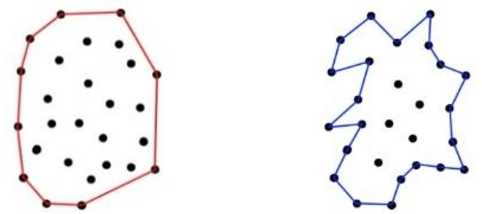
\includegraphics[width=0.8\textwidth]{sections/image/Classification-of-convex-and-concave-hull-Adapted-from-6.png}
    \caption{High(Left) vs Low(Right) Sparsity}
    \cite{sparity-picture}
\end{figure}

\subsubsection{Adaptive Dynamic}
Instead of applying statistics(Section\ref{SDynamic}), a logical step can be added to aid in the dynamic look-ahead process\cite{Strimel2023}. This typically involves an evaluation of the previous iteration(s) \cite{mamou2024dynamicspeculationlookaheadaccelerates} or information gathering\cite {Strimel2023}. 

When evaluating previous iterations, an approach similar to the Lin-Kernighan adaptive selection\cite{Lin1973} can be used(Figure\ref{sporatic}). Changing the depth of look-ahead is beneficial in avoiding local minima that are present within a certain range of depths. By adjusting the depth(Equation\ref{osilatingdepth}), the heuristic can proceed with more promising additions that would have been hindered by pitfalls otherwise.

\begin{equation}
    depth = \min(max\_depth,\  \max(0,\ M\cdot\ln(L\cdot size)\ - C + \tcboxmath[boxmath={red}{displacement}]{D}\cdot\sin(\tcboxmath[boxmath={blue}{sparitrty}]{F\cdot\#iteration}))))
    \label{osilatingdepth}
\end{equation}

\vspace{-0.5cm}

\begin{tikzpicture}[remember picture, overlay, font=\sffamily]
\draw[red,->] (displacement.north) --++(120:5mm) node[anchor=south]{Amplitude};
\draw[blue,->] (sparitrty.north) --++(90:5mm) node[anchor=south]{Frequency};
\end{tikzpicture}

\begin{figure}[]
    \centering
    \resizebox{0.7\textwidth}{!}{%
    \begin{tikzpicture}
        \begin{axis}[
            xlabel={Size}, 
            ylabel={Depth},
            title={Sporadic Depth Function},
            domain=1:500, % Adjust range as needed
            samples=500,
            grid=major,
            thick
        ]
            % Define constants
            \pgfmathsetmacro{\M}{1.235}    % Scaling factor
            \pgfmathsetmacro{\L}{0.906}    % Log multiplier
            \pgfmathsetmacro{\C}{-1.6}    % Offset
            \pgfmathsetmacro{\maxD}{100} % Maximum depth
            
            % Plot the function
            \addplot[blue, thick] {min(\maxD, max(0, round(\M * ln(\L * x) - \C + 2*sin(8*x))))};
            \addplot[black, thick] {\M * ln(\L * x) - \C};
        \end{axis}
    \end{tikzpicture}
    }%
\caption{Plot Of Sporadic Depth Function}
\label{sporatic}
\end{figure}

If acting upon information gathered from the current state, logical assumptions can be used to define the depth. Adding a step that adaptively changes the depth based on the proximity to other nodes can help avoid poor representation in the cost function. A crude method for defining closeness is to count the number of nodes within a specified distance of the node. The closeness cut-off can be defined based on an arbitrary size(Figure\ref {closesearch}), statistical assumptions of the problem(such as the mean value), or the best efforts of previous iterations.

\begin{figure}[H]
    \centering
    \includegraphics[page=13, width=0.8\textwidth]{sections/image/dissertationdemo.drawio.pdf}
    \caption{Closeness Search}
    \label{closesearch}
\end{figure}

\begin{center}
\section{Methodology}
\label{method}
\end{center}

An organised approach to the evaluation and testing is required to study the proposed algorithms analytically. The Travelling Salesman Problem is a single-objective optimisation problem\cite{Halim2021} with the sole goal of minimising the route cost(Equation\ref{TSPcost}). However, it is not the only metric worth considering when evaluating heuristics, as runtime is a major factor in determining which algorithm to use\cite{rardin2001experimental}. Therefore, the data collection method must remain unbiased for the comparisons to have validity.

Empirical research is a research method that involves observing the direct result of an action and gathering data\cite{patten2016proposing}. The values observed are considered empirical data, which can be quantitatively analysed to aid in decision making and reaching a conclusion\cite{patten2016proposing}. Due to the nature of NP-hard problems, it is improbable\cite{Halim2021} to test heuristics against random exact solutions. Therefore, comparing them to other heuristics is an appropriate approach; this is called blind(statistical) testing\cite{BHATTACHARJEE2022100471}.

\subsection{Empirical Testing}

Using large data collection and data analysis, trends and properties are outlined in the testing, which would otherwise be obscured by randomness\cite{BHATTACHARJEE2022100471}. Much like real-life experiments, the collected data(dependent variable) must have controlled variables and a single independent variable. The independent variable is the algorithm and its unique parameters, thus SLACIH(1) and SLACIH(2) are two different independent variable entries. The control is the identical Travelling Salesman Problem and system properties executed for each algorithm. A set of experiments with the same control variable is referred to as an instance. Generating multiple random instances creates a data table in a process known as Instances vs Algorithm\cite{BHATTACHARJEE2022100471}. In the table, all instances must have the same TSP properties, e.g. problem size and random generation method.

\begin{figure}[!ht]
    \centering
    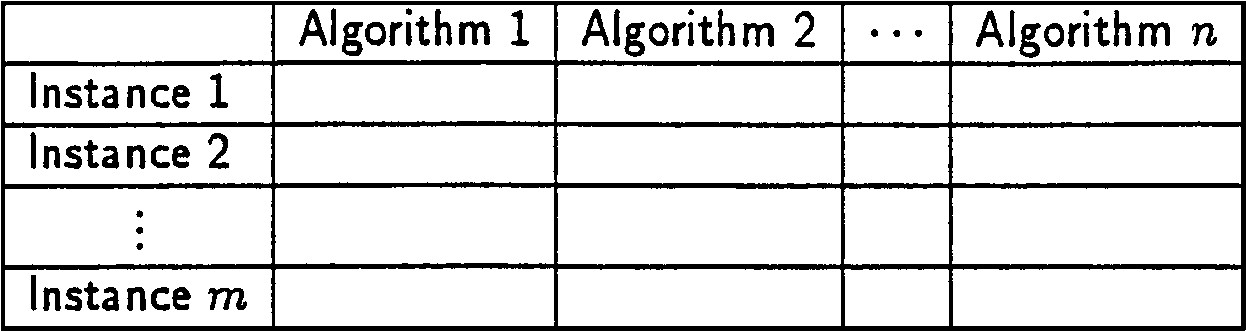
\includegraphics[width=0.7\textwidth]{sections/image/empirical.jpg}
    \caption{Instances Vs Algorithm}
    \cite{rardin2001experimental}
\end{figure}

Once the table has been populated with a sufficient number of instances, to reduce randomness, data analysis can be used to draw conclusions. Statistical properties, such as averages, standard deviation, and inference, are explored as avenues for comparison.

\subsection{TSPLib}

In the research for the Travelling Salesman Problem, there is a library of tests called TSPLib\cite{TSPLIB95}, which contains famous real-world examples and common pitfall problems. It contains 130 problems of varying graph sizes, with the largest having 85,900 nodes. All have been solved with an exact solution by the Concorde TSP Solver(Section\ref{Concorde}), making TSPLib a suitable library for benchmarking heuristics against the global optimal\cite{TSPLibBench}. TSPLib is also useful as a ground truth for comparing research papers due to its ubiquity as a benchmark.

\begin{figure}[H]
    \centering
    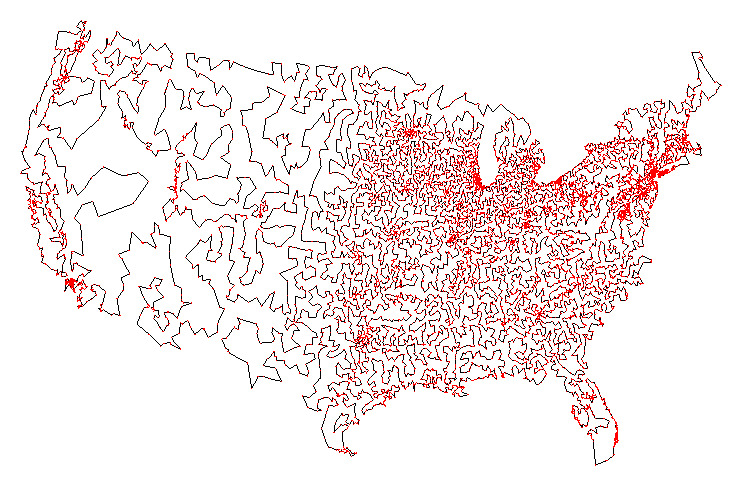
\includegraphics[width=0.7\textwidth]{sections/image/usa13509.sol-ezgif.com-gif-to-jpg-converter.jpg}
    \caption{TSPLib: USA13509} 
    \cite{chvatal2001tsp}
\end{figure}

As the problem solutions vary in cost, taking the difference from the optimal solution as a percentage(Equation\ref{psolution}) allows for calculating the average performance of a heuristic across the entire TSPLib(Equation\ref{ptsplib}). This normalisation allows for each problem to contribute evenly to a heuristic score.

\begin{equation}
    p_{solution}=\frac{solution_{heuristic}-solution_{optimal}}{solution_{optimal}}
    \label{psolution}
\end{equation}

\begin{equation}
    p_{TSPLib}=\frac{\sum{p_{solution}}}{|p_{solution}|}
    \label{ptsplib}
\end{equation}
\begin{center}
\section{System Requirements}
\label{sec:system}
\end{center}

Until this point, the report has primarily focused on research and theoretical designs, but software development is a significant aspect required to prove and analyse the theory. Making the right system design choices is crucial to the success of the project's aims and goals, ensuring that valuable time is not wasted on refactoring and bug fixing. Multiple working computer programs are required to fill all the project needs; therefore, the code should be adaptable and highly interoperable. The programs should utilise state-of-the-art technology to leverage all the benefits to achieve the highest success. Planning and system requirements are crucial, as most IT projects fail because there were not clearly defined requirements\cite{functional_requirements}.

\subsection{Functional Requirements}
\label{sec:requirements}
Functional requirements define what the product(s) should do regarding behaviour and features; achieving these requirements is essential for the project's success. Each requirement can be classified by type, description, and aim in Table\ref{tab:functionalreq}.
\pagebreak

\begin{table}[!ht]
    \centering
    \renewcommand{\arraystretch}{1.2} % Adjust row height for readability
    \begin{tabularx}{\textwidth}{
    |>{\raggedright\arraybackslash}p{3cm}
    |>{\raggedright\arraybackslash}p{1.3cm}
    |>{\raggedright\arraybackslash}p{4cm}
    |>{\raggedright\arraybackslash}X|}
\hline
\multicolumn{1}{|c|}{{\ul \textbf{Name}}} & \multicolumn{1}{c|}{{\ul \textbf{Type}}} & {\ul \textbf{Description}}               & {\ul \textbf{Aim}}                                                                                                          \\ \hline
1.a) Graph Theory                              & Data                                     & Store vertices and edges                    & The program should be able to handle storing any number of vertices and edges in memory as mentioned in Section\ref{graph_data} \\ \hline
1.b) TSP Constraints                           & Logic                                    & Follow the rules of a TSP problem           & The program should not break any of the TSP constraints mentioned in Section\ref{hamiltonian-data}                                                \\ \hline
1.c) Euclidean TSP                             & Logic                                    & Follow the rules of a Euclidean distance    & The program should calculate the Euclidean distance correctly between two vertices                                          \\ \hline
2.a) Facilities for Algorithms                 & Logic                                    & Allow multiple algorithms to be used        & The program should be able to be used for numerous algorithms                                                               \\ \hline
2.b) Benchmarking Algorithm                    & System                                   & Benchmarking of route length and time taken & The program should accurately report and store the results of an algorithm execution                                         \\ \hline
2.c) Algorithm Fairness                        & Perfor-
mance                              & All algorithms should operate at their best & The program should not negatively impact the performance of an algorithm \\ \hline
2.d) Testing Suite                             & System                                   & Allow for multiple different types of tests & The program should be able to run various types of tests with many parameters repetitively and for long periods \\ \hline
3.a) Display TSP Solutions                     & UI/UX                                    & GUI output of the algorithms solutions      & The program should adequately display graphs and Hamiltonian cycles                                                         \\ \hline
4.a) Collect Test Data                         & Data                                     & Collect multiple instances of test data     & The program should use secondary storage, a proper text-based formatting system                                             \\ \hline
4.b) Analysis Test Data                        & System                                   & Produce statistics and graphs               & The program should provide data analysis on the collected data to produce meaningful statistical insight                    \\ \hline
5.a) Unit Test                                 & System                                   & Adequately unit test code base              & The program should have unit test coverage of the core shared library codebase, focusing on systems used by every component \\ \hline

    \end{tabularx}
    \caption{Functional Requirements}
    \label{tab:functionalreq}
\end{table}
\pagebreak

\subsection{Non-Functional Requirements}

Non-functional requirements define the level of quality the product(s) should have in terms of behaviour and features; achieving these requirements is not essential for the project's success but would be beneficial. Each requirement can be classified by its aim and type in a table.
\vspace{0.4cm}
\begin{table}[!ht]
    \centering
    \renewcommand{\arraystretch}{1.2} % Adjust row height for readability
    \begin{tabularx}{\textwidth}{|X|p{3cm}|}
    \hline
{\ul \textbf{Aim}}                                                                         & {\ul \textbf{Type}} \\ \hline
The user should be able to select the type of algorithm they want easily                   & Usability           \\ \hline
The program should never fail or crash                                                     & Reliability         \\ \hline
The program should be responsive and utilise all computing power                           & Performance         \\ \hline
The program should be adaptable and fill the needs of each executable                      & Scalability         \\ \hline
The GUI should be easy to read for all users, e.g. inclusive of those with colour blindness & Usability           \\ \hline
    \end{tabularx}
    \caption{Non-Functional Requirements}
    \label{tab:nonfunctionalreq}
\end{table}

\subsection{C++}
\label{sec:c++}
C++ is a low-level programming language first created in 1985 by Bjarne Stroustrup\cite{stroustrup2013cpp}. It is widely used in algorithmic research and industry due to its high performance and low-level capabilities. In this project, C++ was selected as the primary language due to prior experience and previous personal projects involving the language. MSVC\cite{visualstudio_cpp} compiler was used as it integrates seamlessly with Visual Studio and C++20\cite{cppreference_cpp20} for it is the most modern long-term support(LTS) version.

C++ has no built-in memory management and relies on the programmer to handle allocation and deletion. This removes the overhead of an automatic memory management system but can lead to data corruption or memory violations. The benefit of allowing the programmer to decide is the ability to use either stack vs heap memory.
\begin{itemize}
    \item Stack: Faster but limited by size and must be known at compile time
    \item Heap: Unlimited size and can be dynamically allocated, but slower as it requires OS system call and uses a pointer to access.
\end{itemize}

Accessing memory is a leading cause of slow performance times due to cache misses \cite{drepper2007memory}. C++ has low-level calls that are unique to low-level languages, allowing for direct manipulation of computer memory. This allows for logical memory tricks and greater control over memory to accommodate each system's architecture\cite{memorymanagement}. Both must be used when programming in C++, but stack memory is favourable in most situations.

Object-Oriented Programming(OOP) has become the standard programming paradigm for most use cases. OOP is dynamic as encapsulation and polymorphic properties can be applied to most problems. The abstract nature and use of Creational Patterns lend OOP well to this project for initiating multiple algorithms.  

\subsubsection{API \& Interfaces}
\label{sec:API}

To satisfy the multiple functional requirements(Table\ref{tab:functionalreq}), various computer programs(executables) will need to be developed to achieve each of the different requirements. Each program will require the same features and data, so to avoid bugs and repetitive code; core functionality is placed in a library. There are two types of libraries in C++:

\begin{itemize}
    \item Static Library: Library code is added to the source code and compiled at compile time
    \item Dynamic Library: Library code is compiled into a DLL and linked at run-time
\end{itemize}

The benefits and differences depend on a few factors, but the static library was preferred due to template metaprogramming(Section\ref{template}). However, both remove the dependency of an owner, and a static library acts as the project's base. To ensure practical software development, it is still essential to understand how the library functions and interacts with each program; this is achieved by following standard Design Patterns, APIs, and Interfaces.

As seen in Section\ref{lit}, several stages and optimisations can be applied to create an overall heuristic, including tour constructors, tour optimisers, partitioning systems, and caching modes. To construct any number of combinations by hand would be infeasible, so a Creational Pattern in OOP, called a Builder\cite{refactoringGuruBuilder}, is used like a cookie cutter for each option. The idea is to have a single Builder class that utilises composition to construct the algorithm for the possibilities it provides. This requires interfaces for the builder class to call upon its objects.

\begin{figure}[H]
    \centering
    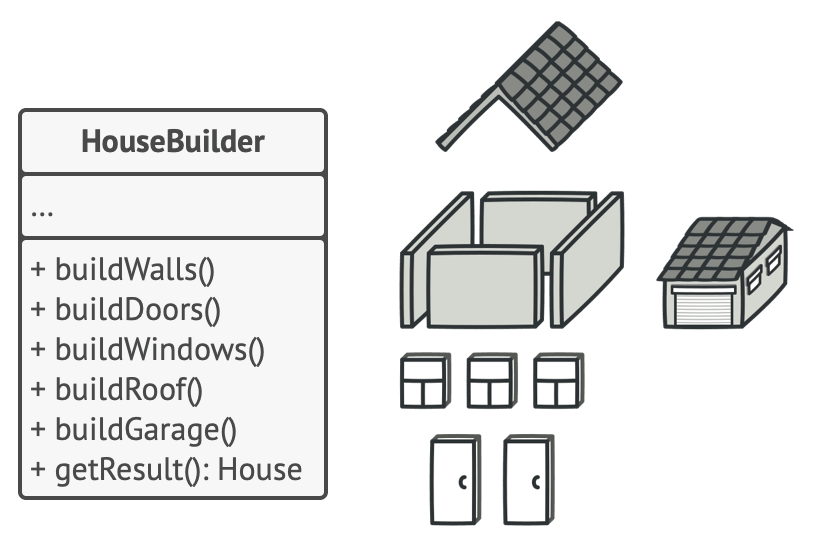
\includegraphics[width=0.5\textwidth]{sections/image/Builder.png}
    \caption{Builder Pattern}
    \cite{refactoringGuruBuilder}
\end{figure}

Interfaces are public abstract classes that utilise the polymorphic nature. Abstract classes cannot exist as objects due to being incomplete classes, but they can be inherited by child classes to gain their properties. This ensures that each built object has the correct interface for immutability within the larger system.

To ensure the user(programmer) does not interact with the library incorrectly, APIs are used to limit the control they have over the underlying data. API's also help programmers more easily understand what the code is doing and what the original creator had in mind. APIs are heavily relied upon for communication between the library and each executable.

\subsubsection{Template Metaprogramming}
\label{template}

Template Metaprogramming(TMP) is an additional step in the C++ compiler that introduces compile-time polymorphism by utilising template functions\cite{vandevoorde2002c++}. It allows a single template function to have infinite copies of itself without requiring additional code. Template functions require a template variable, which takes the values of data types, functions, or constant values. At compile time, the template function variables are instantiated in the template functions to create inlined generic source code.

\begin{lstlisting}[caption={Template Code}, label={fig:template},numbers=left]
template<typename var>
void foo(var a) {
    std::cout << "value : " <<  a << "\n";
}

/*
What the compiler would generate:

void foo<int>(int a) {
    std::cout << "value : " <<  a << "\n";
}

void foo<std::string>(std::string a) {
    std::cout << "value : " <<  a << "\n";
}
*/

template<int var>
class goo {
public:
    static void bar() {
        std::cout << "value : " << std::to_string(var) << "\n";
    }
};

/*
What the compiler would generate

static void goo<5>::bar() {
    std::cout << "value : " << std::to_string(5) << "\n";
}
*/

int main()
{
    foo<int>(10);                 // print "value : 10"
    foo<std::string>("hello");  // print "value : hello"
    
    goo<5>::bar();                // print "value : 5"
}
\end{lstlisting}

In the example, Listing\ref{fig:template}, $foo()$ is a template function, and var is a template function variable. In the $main()$ function, foo is instantiated with the data types $int$ and $string$, and then arguments of those types are passed. The program compiles and runs as expected, with the $foo<int>()$ and $foo<string>()$ functions being generated before compile time, as represented by the code in the comment(Line 9). Classes can also have templates, which can define member fields and functions(Listing\ref{fig:templateAdv}).

\begin{lstlisting}[caption={Advance Template Code}, label={fig:templateAdv},numbers=left]
class abstract {                    // Pure abstract class 
    virtual void foo() = 0;
};

class child : public abstract {    // Abstract child class
    void foo() override {
        std::cout << "real function";
    }
};

template<typename T>
class real {
    static_assert(std::is_base_of<abstract, T>::value, "T must derive from abstract");
    
    T var;  // Compile-Time Polymorphism: In-line real class without V-Table
};

int main() {
    real<child> b;    // Abstract class on the stack
}
\end{lstlisting}

Metaprogramming has its roots in compiler development but is heavily applied in performance optimisation code. This is because a constant expression can be evaluated at compile time, leading to the removal(inlining) of branching and expression evaluation. Much like its name, compile-time polymorphism, metaprogramming\cite{abrahams2004c++} can mimic OOP polymorphism at compile time(Listing\ref{fig:templateAdv}). This is faster than normal polymorphism, as it eliminates the V-Table, which determines which child virtual function to invoke. Calling the V-Table incurs a constant time slowdown, which is undesirable when performance is a concern and the number of calls varies between TSP algorithms.

\begin{figure}[!ht]
    \centering
    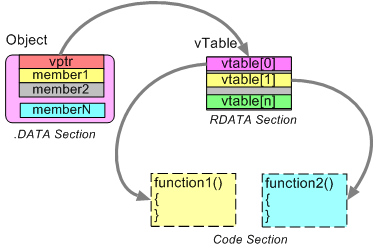
\includegraphics[width=0.7\textwidth]{sections/image/vptr-vtable-vfunctions.png}
    \caption{C++ V-Table}
    \cite{refactoringGuruBuilder}
\end{figure}

Another performance benefit of TMP is compile instantiation. Many data types must be placed on the heap due to their dynamic size, which incurs a performance hit with each call. As TMP instantiates classes with the type in place at compile time, it can allocate a static size on the stack for abstract child classes, thereby avoiding any performance hit(Listing\ref{fig:templateAdv}). 

As this project is heavily performance-focused, fairness is necessary; not using templates would be a mistake. Compile-time polymorphism enables builder classes with constant slowdowns to behave like a monolithic class, allowing in-line and optimisation of function calls. Templates have their disadvantages, including steep learning curves, reduced flexibility, additional complexity, difficult to debug, long compilation times, and memory usage issues; however, these are negligible for the scale and scope of this project.

\subsubsection{QT6}

QT\cite{qt6} is a cross-platform GUI library for creating graphical applications natively on all operating systems and embedded hardware. It is written in C++ but can also be developed with Python. QT6 is the most modern iteration, having undergone 29 years of development and featuring an open-source license, making it a go-to choice for research and non-profit developers. The needs of this project do not necessitate a wide use of graphical features, which is why choosing QT6, with its extensive catalogue of tutorials, was ideal.

\begin{figure}[!ht]
    \centering
    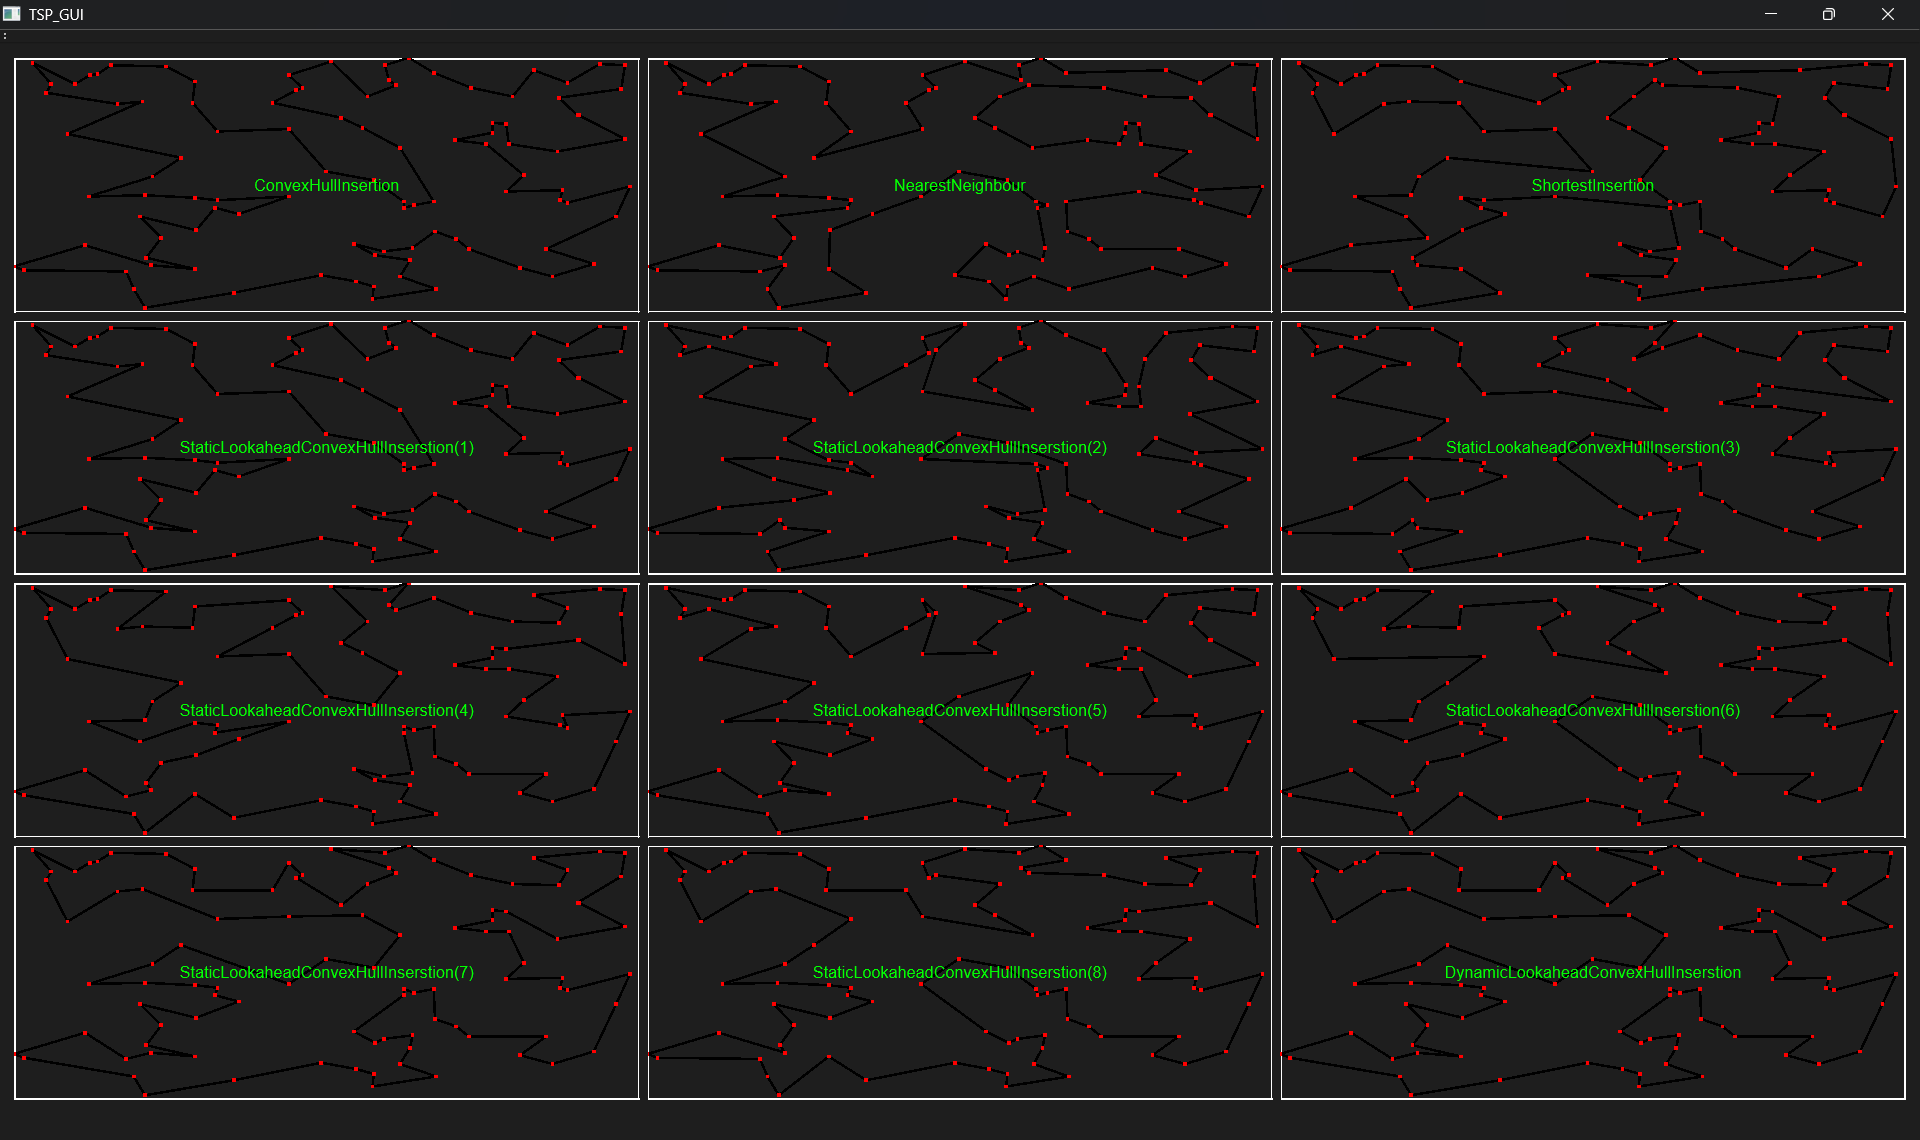
\includegraphics[width=\textwidth]{sections/image/Result.png}
    \caption{Example: QT6 Application GUI}
\end{figure}

\subsubsection{C++ Libraries}
\label{cpplibrar}
Libraries are valuable resources for ontaining a pre-made solution to complex functionality that developers widely encounter. However, when C++ was being developed, library support and development were not as prolific as modern languages. For this project, the libxlsxwriter library\cite {libxlsxwriter} helped generate Excel files. GNU Scientific Library\cite{gsl} was used for the gradient descent function in optimising the dynamic look-ahead arguments. 

\subsection{Hardware}

Hardware is a crucial factor in testing NP-hard problems; from tiny microcontrollers to massive supercomputers, the amount of available computing power determines the problem size and the type of algorithm that can be used. The project was completed using a home desktop PC running Windows 11, equipped with an Intel i9-13900 processor and 32GB of RAM. 

\subsubsection{Consistency}

For the fair testing of algorithms(Section\ref{method}), physical and external factors need to be controlled as a control variable to prevent bias. Physical factors comprise of power draw to thermal temperatures, while external factors include background tasks and execution mode. With no funding or external resources, controlling many of the variables was hindered.

Thermal temperatures of the CPU constitute the most significant downfall; excessive heat can trigger thermal throttling, reducing performance. Managing thermal temperatures with effective cooling systems and maintaining a consistent ambient temperature was not possible with the available setup. Therefore, overclocking the CPU was disabled to maintain a stable clock rate for extended periods.

When compiling the program, the identical execution flags and release mode should be constant. Tests should not be run quickly after boot or with background tasks running, as these may consume CPU time.

\subsubsection{Multi-Threading}

To fulfil the non-functional requirements(Table\ref{tab:nonfunctionalreq}) and reduce the time required to gather all the data, tests are run in parallel. Each process also uses asynchronous timeout calls to prevent tests from running indefinitely. Therefore, a multi-core processor is a requirement for achieving stable performance.

\subsubsection{Memory}

The Travelling Salesman Problem and look-ahead design can consume a significant amount of memory if the problem is sufficiently large. With modern hardware storing GB of RAM and MB of cache, the space capacity is not likely to be a limiting factor. However, the constant reading and writing of memory can hinder performance; therefore, quicker RAM is favourable.

\begin{center}
\section{Design}
\label{design}
\end{center}

Breaking the problem down into building blocks of abstract classes and interfaces allows each system to define how it should interact and behave. As mentioned in Section\ref{sec:API}, creational patterns are valuable techniques for constructing large-scale systems. Combining Builder classes and API is the basis for how the system is structured.

\begin{figure}[H]
    \centering
    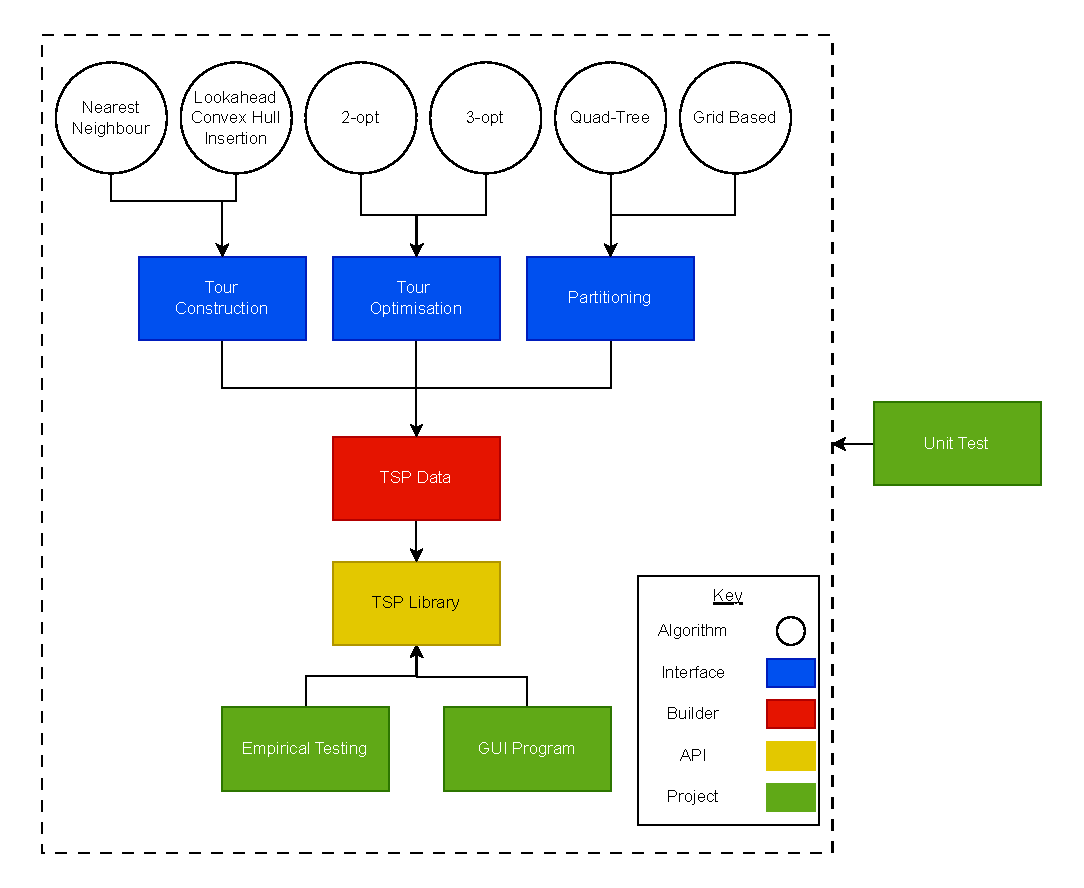
\includegraphics[width=1\textwidth]{sections/image/Class_Diagram-Basic.drawio.pdf}
    \caption{Class Structure}
    \label{fig:classdia}
\end{figure}

Figure\ref{fig:classdia} illustrates the class hierarchy and the interactions between each system block for the core static library code. At each level, a layer of abstraction is applied to hide information about the other blocks, allowing them to work independently.

\subsection{TSP Library API}
\begin{figure}[H]
    \centering
    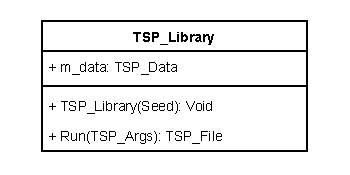
\includegraphics[width=0.6\textwidth]{sections/image/Class_Diagram-TSP_Lib.drawio.pdf}
    \caption{TSP Lib}
    \label{fig:TSP_Lib}
\end{figure}

The TSP Library serves as the entry point for the static library, providing the API that controls the creation and execution of TSP algorithms through the TSP\_data class. It is responsible for parsing the data and serialising the result. It houses all the asynchronous timeout code and benchmarking functionality.

There are only two functions: the constructor and the run function. The constructor uses a seed value to generate m\_data as a composition object with all the data required for the functionality. The run function controls the handling of timeouts, the execution of the algorithm steps, and data serialisation to the TSP\_File type. The ordering of the run function is as follows:

\begin{enumerate}
    \item Start benchmark timer
    \item Initialise partitioning data
    \item Initialise caching data
    \item Run tour constructor algorithm
    \item Run tour optimiser algorithm
    \item Stop benchmark timer
    \item Validate the route
    \item Process data and serialise to TSP\_File
\end{enumerate}

\subsubsection{TSP File}
\label{sec:TSP_File}
\begin{figure}[H]
    \centering
    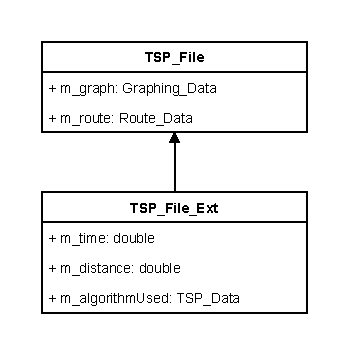
\includegraphics[width=0.5\textwidth]{sections/image/Class_Diagram-TSP_File.drawio.pdf}
    \caption{TSP File}
    \label{fig:TSP_File}
\end{figure}

TSP\_File represents multiple classes for deserialising and serialising the `.TSP' file type, which originates from the TSPLib format. The original file type contains relevant information to reconstruct the problem and its solution. For this project, the file type was expanded using polymorphism by adding benchmarking statistics with the class TSP\_File\_Ext.

\subsection{TSP Data API}
\label{tspData}

\begin{figure}[H]
    \centering
    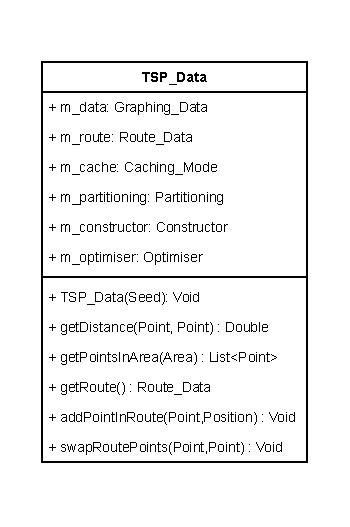
\includegraphics[width=0.5\textwidth]{sections/image/Class_Diagram-TSP_Data.drawio.pdf}
    \caption{TSP Data}
    \label{fig:TSP_Data}
\end{figure}

TSP\_Data is what connects everything together and ensures the TSP properties are kept. It is a builder class(Section\ref{sec:API}) for generating any variation of TSP algorithm from the number of TSP Modules(Section\ref{modules}). It stores the graph theory and route creation data and logic, serving as an API(Table\ref{tab:functions}) for the composition objects and forcing them to utilise the caching(getDistance) and partitioning(getPointsInArea) techniques. The class isolates the raw data from other classes to prevent data corruption and ensure the properties of the Travelling Salesman Problem(addPointInRoute \& swapRoutePoints) are maintained. The tour constructor uses the addPointInRoute() function, and tour optimisers uses swapRoutePoints(), as seen from Figure\ref{twosubprocedure}.

\begin{table}[H]
    \centering
    \renewcommand{\arraystretch}{1.2} % Adjust row height for readability
    \begin{tabularx}{\textwidth}{|p{3.2cm}|p{2.5cm}|p{2.5cm}|X|}
\hline
{\ul \textbf{Function}} & {\ul \textbf{Argument}} & {\ul \textbf{Return}} & {\ul \textbf{Description}}                                                       \\ \hline
TSP\_Data()             & Random Seed             & Void                  & Constructor: Generate a random problem                                           \\ \hline
getDistance()           & Point \& Point          & Double      & Checks the cache table or generates the Euclidean distance between two points         \\ \hline
getPointInArea()        & Area                    & List of Points        & Uses the partitioning algorithm to fetch all the points within a geographical area \\ \hline
getRoute()              & Null                    & List of Points        & Returns current route                                                            \\ \hline
addPointInRoute()       & Point \& Position       & Null                  & Adds point to the position in the route                                          \\ \hline
swapRoutePoints()       & Point \& Point          & Null                  & Swaps two points in the route                                                    \\ \hline
    \end{tabularx}
    \caption{Function Definition}
    \label{tab:functions}
\end{table}


\subsection{TSP Modules Interfaces}
\label{modules}

Interfaces or pure virtual classes in C++(Section\ref{sec:API}) dictate the interaction through which to communicate with a block. The interface acts as a conduit between TSP\_Data and the underlying algorithms and functionality(Figure\ref{fig:modules}). Because the modules only need to interact statically with TSP\_Data and they are situated in composition, a reference is all that is required for modules to access the API(Section\ref{tspData}).

\begin{figure}[H]
    \centering
    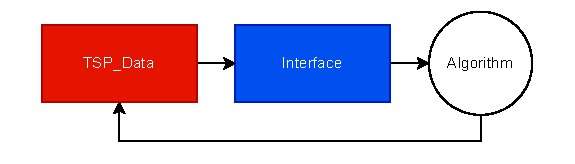
\includegraphics[width=0.7\textwidth]{sections/image/Class_Diagram-Page-5.drawio.pdf}
    \caption{Modules Interface Interaction}
    \label{fig:modules}
\end{figure}

The program employs this technique in four locations: the tour constructor, the tour optimiser, partitioning, and caching. For tour constructors and optimisers, the interface handles the uniform construction and destruction of every algorithm through a base process, runConstructor() and runOptimiser(). The partitioning interface requires the underlying partition type(Section\ref{partitioning}) to have both a construction method and a method for determining points within an area. Caching similarly requires a construction method and a distance between points. Interfaces are a requirement because each implementation utilises a distinct memory structure and logic to achieve the same functionality, as shown in Figure\ref{fig:part_example}.

\begin{figure}[H]
    \centering
        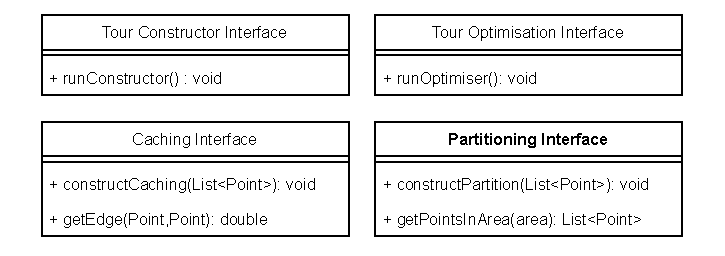
\includegraphics[width=\textwidth]{sections/image/Class_Diagram-Page-7.drawio.pdf}
        \caption{Interface Descriptions}
    \label{fig:}
\end{figure}

\begin{figure}[H]
    \centering
    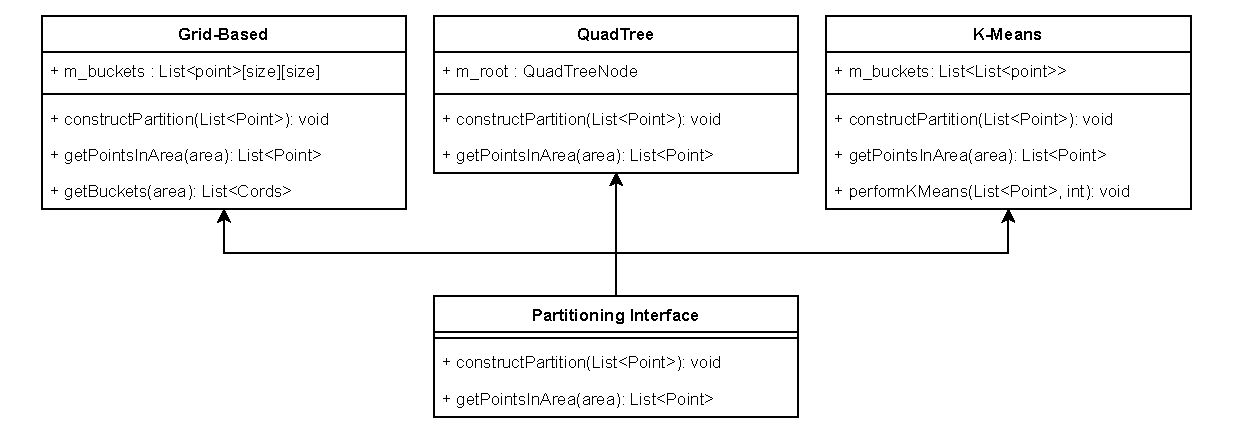
\includegraphics[width=\textwidth]{sections/image/Class_Diagram-Page-6.drawio.pdf}
    \caption{Partitioning Interface Example}
    \label{fig:part_example}
\end{figure}

\subsection{TSP Projects}

Projects are individual executables that compile shared and discrete code independently, each with its own set of compiler options and libraries. Mixing GUI applications and background applications presents numerous issues and increases complexity when the two applications are disjointed. Therefore, keeping each application's specific code and compiler options separate improves development time and user application efficiency. If the applications require shared code, that shared code should be placed in a static library(Section\ref{sec:c++}), which is what the TSP Library is. This report requires four projects: Empirical Testing Suite, GUI output, Unit test, and TSP File Reader.

\subsubsection{Empirical Testing Suite}
\label{sec:testing}
The Empirical Testing Suite is a Command-Line Interface(CLI) application for selecting and starting the process of testing various algorithms, serving as the primary component of the report and following the methodology listed in Section\ref{method}. It supports simultaneous testing and multiple test suite designs. It is responsible for creating, appending, and saving the result data to a file(More in Section\ref{filesystem}). There are multiple different test suites that serve different purposes:

\begin{table}[H]
    \centering
    \renewcommand{\arraystretch}{1.2} % Adjust row height for readability
    \begin{tabularx}{\textwidth}{|p{3cm}|X|X|}
    \hline
{\ul \textbf{Name}}           & {\ul \textbf{Function}}                                   & {\ul \textbf{Aim}}                                                             \\ \hline
Basic Test                    & Runs every algorithm for a given problem size             & Generates simple data for each algorithm                                             \\ \hline
Multi Test                    & Runs every algorithm for multiple different problem sizes & Generates a wide range of data for every algorithm                                   \\ \hline
Dynamic Test                  & Runs only SLACIH and DLACIH for a given problem size      & Generates data for the optimal depth of SLACIH and comparative performance of DLACIH \\ \hline
Dynamic Args Gradient Descent & Performs gradient descent on DLACIH arguments             & Hyper-optimise the DLACIH arguments values                                                \\ \hline
TSPLib Test                   & Runs DLACIH on every Euclidean TSP in TSPLib              & Benchmark DLACIH against exact solutions                                       \\ \hline
    \end{tabularx}
    \caption{Test Suites}
    \label{tab:testsuites}
\end{table}

\begin{figure}[H]
    \centering
    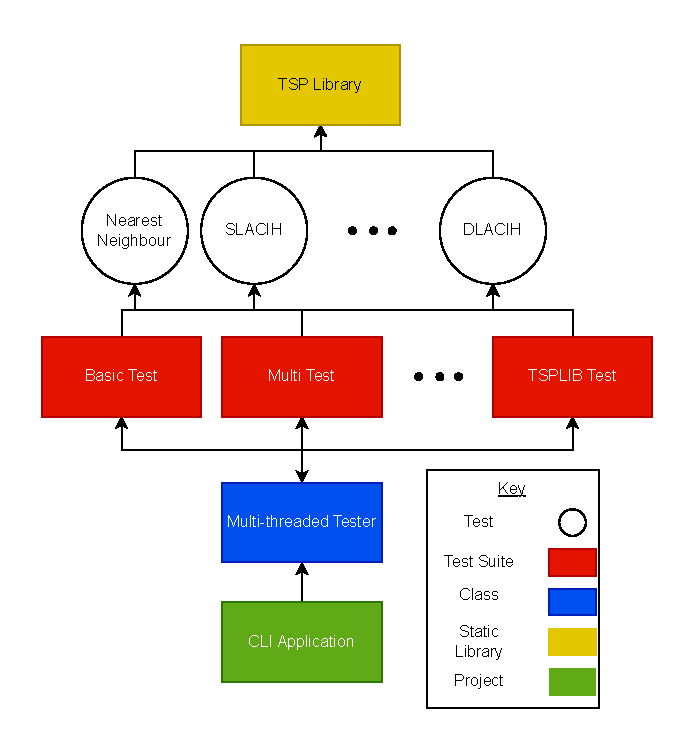
\includegraphics[width=0.75\textwidth]{sections/image/Class_Diagram-Page-8.drawio.pdf}
    \caption{Empirical Testing Suite Design}
    \label{fig:Emprical}
\end{figure}

The application block serves as the entry point, featuring only CLI menu logic and basic sanitation checks. It passes on the user inputs to the multi-threaded tester for execution. The menu collects inputs such as:
\begin{itemize}
    \item Which test suite to run
    \item How many iterations to run
    \item How long it should run for 
    \item What file type should it produce
\end{itemize}

The multi-threaded tester(Tester for short) is the core block, as it allows other classes to add tests to a queue for them to be run in parallel and adheres to the parameters set by the user. The Tester features an iterative, asynchronous loop that manages the continuous execution of the selected test suite and periodically writes the results to a file(Section\ref{filesystem} \& Figure\ref{fig:emp_scr}). The Tester limits the number of active tests to the number of cores available and executes a new test only once a thread from the active thread pool becomes available in a FIFO queue. Equipped in the terminal is a CTRL+C break command to gracefully stop the test mid-run, preventing file corruption.

\begin{figure}[H]
    \centering
    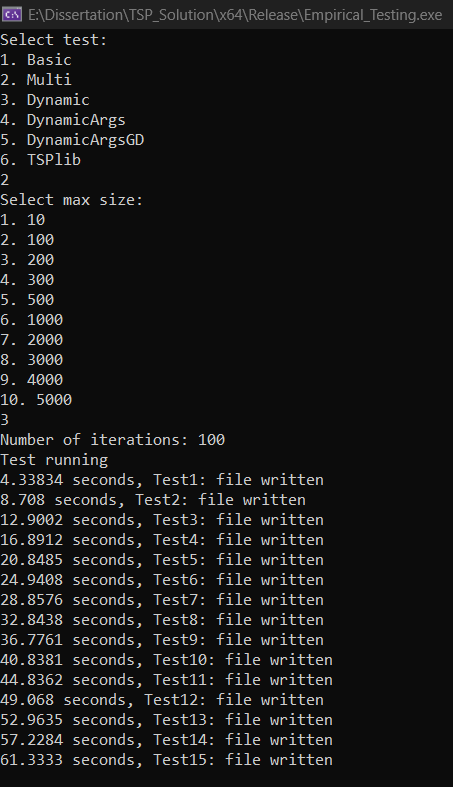
\includegraphics[width=0.35\textwidth]{sections/image/Screenshot 2025-04-08 111230.png}
    \caption{Empirical Test Suite}
    \label{fig:emp_scr}
\end{figure}

The test blocks(black circle in Figure\ref{fig:Emprical}) are individual tests that act as a wrapper(also known as an adaptor) for running an algorithm on the TSP Library with some given parameters. The test suite blocks(red rectangles in Figure\ref{fig:Emprical}) are predefined sets of tests that load the test blocks into the multi-threaded tester. Each test suite has a design it is trying to evaluate, and they do not behave equally. The test suite TSPLIB does not use random problems and instead solves the Euclidean TSP contained in TSPLIB from the smallest to the largest problem. The test suite Dynamic Args Gradient Descent(Table\ref{tab:testsuites}) uses the same five problems for each iteration of the gradient descent.

\subsubsection{TSP GUI}
\begin{figure}[H]
    \centering
    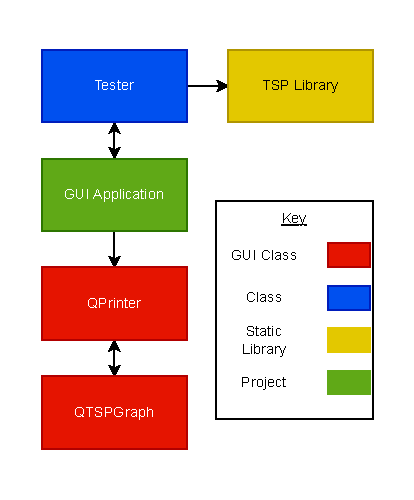
\includegraphics[width=0.5\textwidth]{sections/image/Class_Diagram-Page-9.drawio.pdf}
    \caption{TSP GUI Design}
    \label{fig:guidesign}
\end{figure}

Euclidean TSP belongs to the geometric space, therefore, the points and edges of the graph problem can be represented on a two-dimensional plane. This can be displayed on a GUI application to verify and analyse solutions. This is achieved through QT6 and a paint system for drawing diagrams(Figure\ref{fig:TSPGUI}). The GUI application runs in two steps: it runs algorithms on a TSP, then displays the solution. The two steps do not interact, apart from passing the backend output into the frontend(Figure\ref{fig:guidesign}).

\begin{figure}[H]
    \centering
    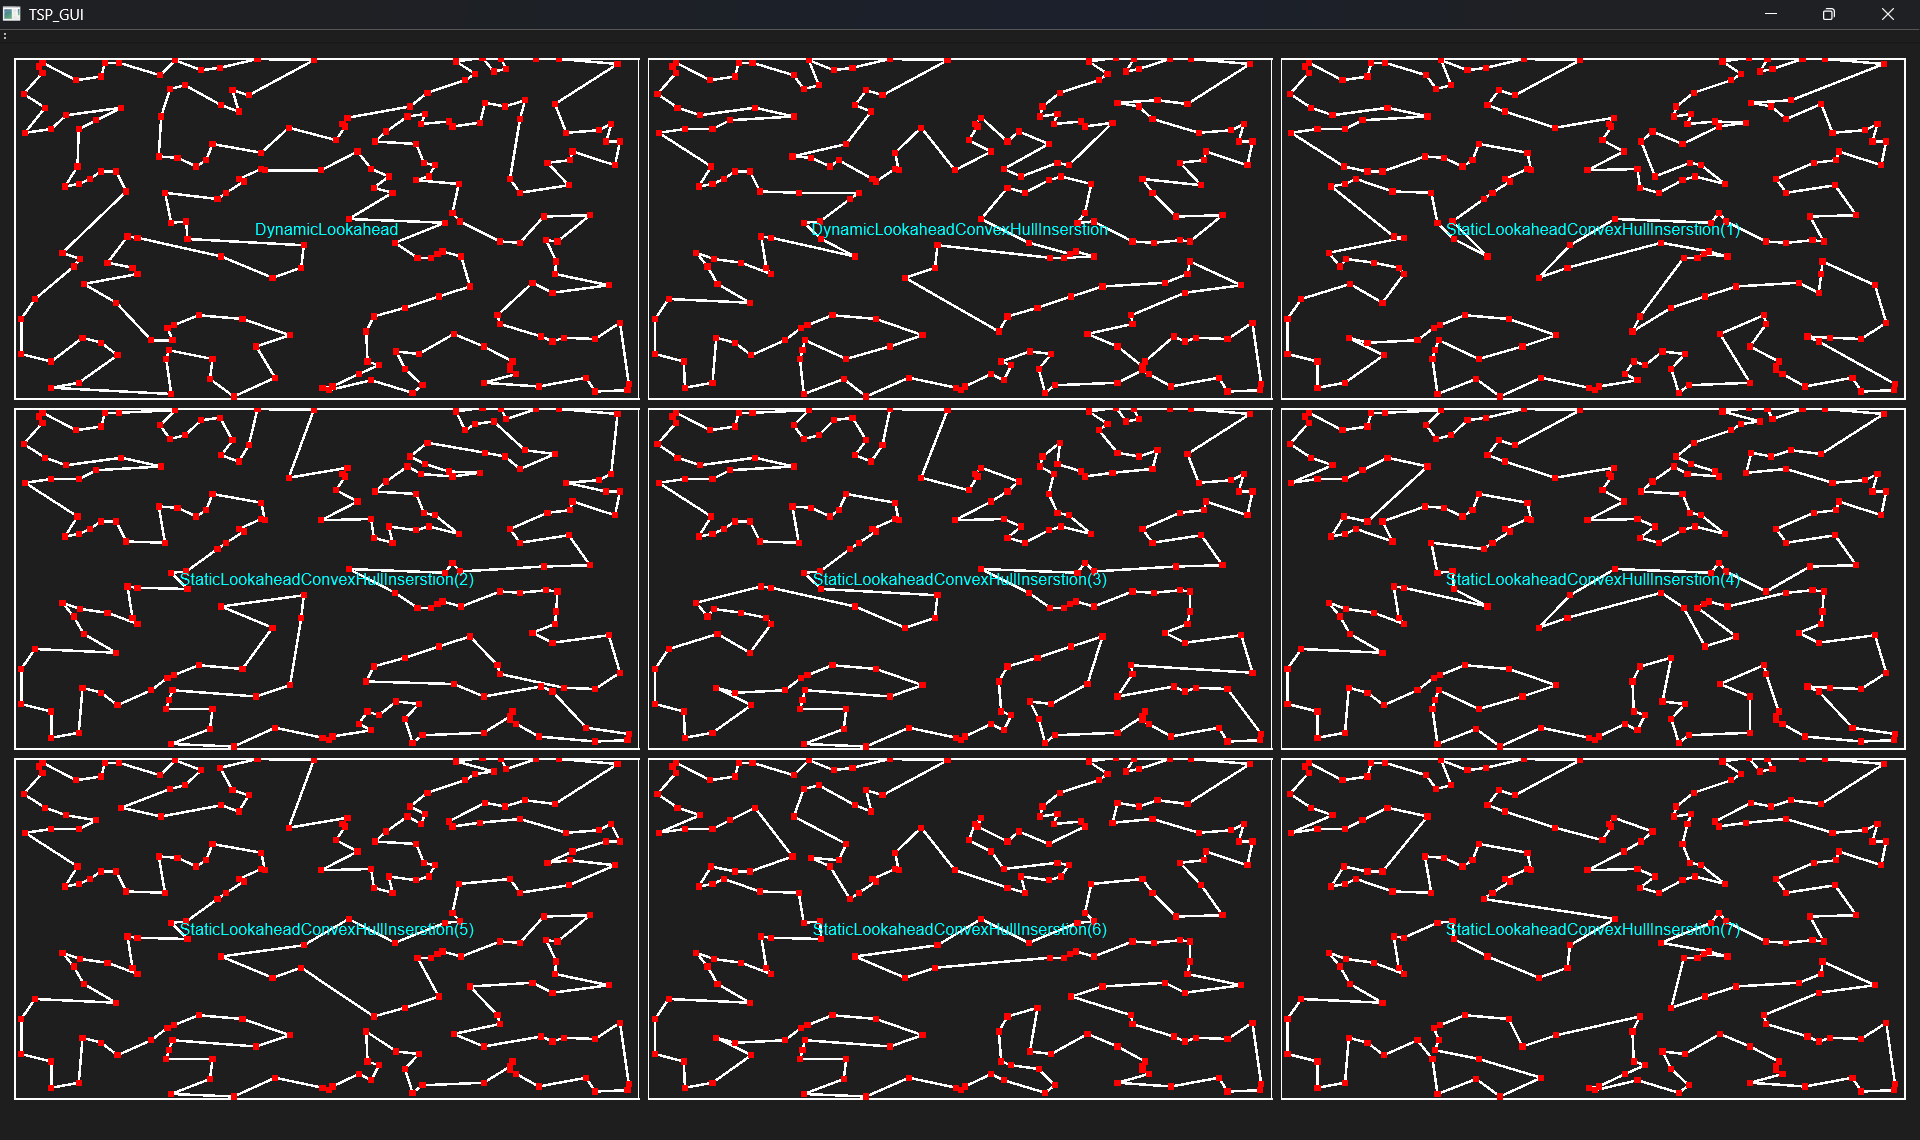
\includegraphics[width=0.95\textwidth]{sections/image/TSP_GUI.png}
    \caption{TSP GUI}
    \label{fig:TSPGUI}
\end{figure}



\subsubsection{Unit Test}
\label{designUnit}
C++ has a plethora of unit testing libraries, all with their pros and cons, but there are no wrong choices. GoogleTest\cite{googletest} is used for its simple integration into Visual Studio. In Figure\ref{fig:classdia}, the unit test encapsulates the entire code base as it can access and create any object needed for the test. This project followed the ``art of unit testing"\cite{osherove2013art} design for a good unit test, reducing complexity by testing only one variable and ensuring repeatable and predictable results.

\begin{figure}[H]
    \centering
    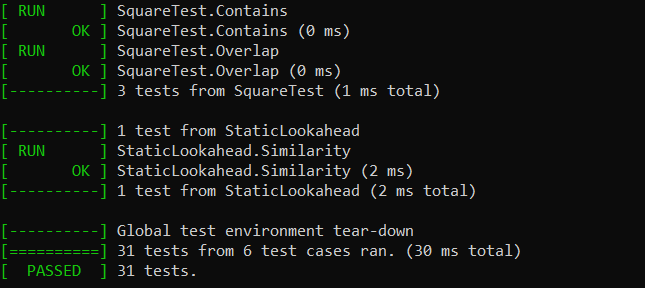
\includegraphics[width=0.6\textwidth]{sections/image/Unit.png}
    \caption{Unit Test Completion}
\end{figure}

\subsubsection{TSP File System}
\label{filesystem}

Tsp\_file(Section\ref{sec:TSP_File}) refers to the naming convention and type of data that is being stored. For the use-case of storing test results, the file needs to be stored in a dynamically sized list of tsp\_file entries for appending and reading the results. No standard exists, so the choice of file format is made by the developer. Text-based formats like JSON\cite{rfc8259} are human readable and scheme free. C++ does not have the modern compiler reflection feature\cite{reflectiveprogramming}, which would allow the compiler to modify its own behaviour based on its own code. This feature is used by most JSON libraries outside C++ to serialise and deserialise class structure automatically; for C++, the conversion has to be manually defined which could introduce errors if not adequately tested.

The files produced by the empirical testing are illegible for human use due to excessive data in an illogical format. Therefore, an application, TSP\_Reader, that can deserialise, analyse, and reproduce more legible data is beneficial. TSP\_Reader uses the TSP file system to process the file, uses data processing to transform the data into a more readable form, and then uses the libxlsxwriter library(Section\ref{cpplibrar}) to create an Excel file with tables and graphs. The data is processed based on problem size(Figure\ref{Excel1}) and algorithm(Figure\ref{Excel2}).

\begin{figure}[H]
    \centering
    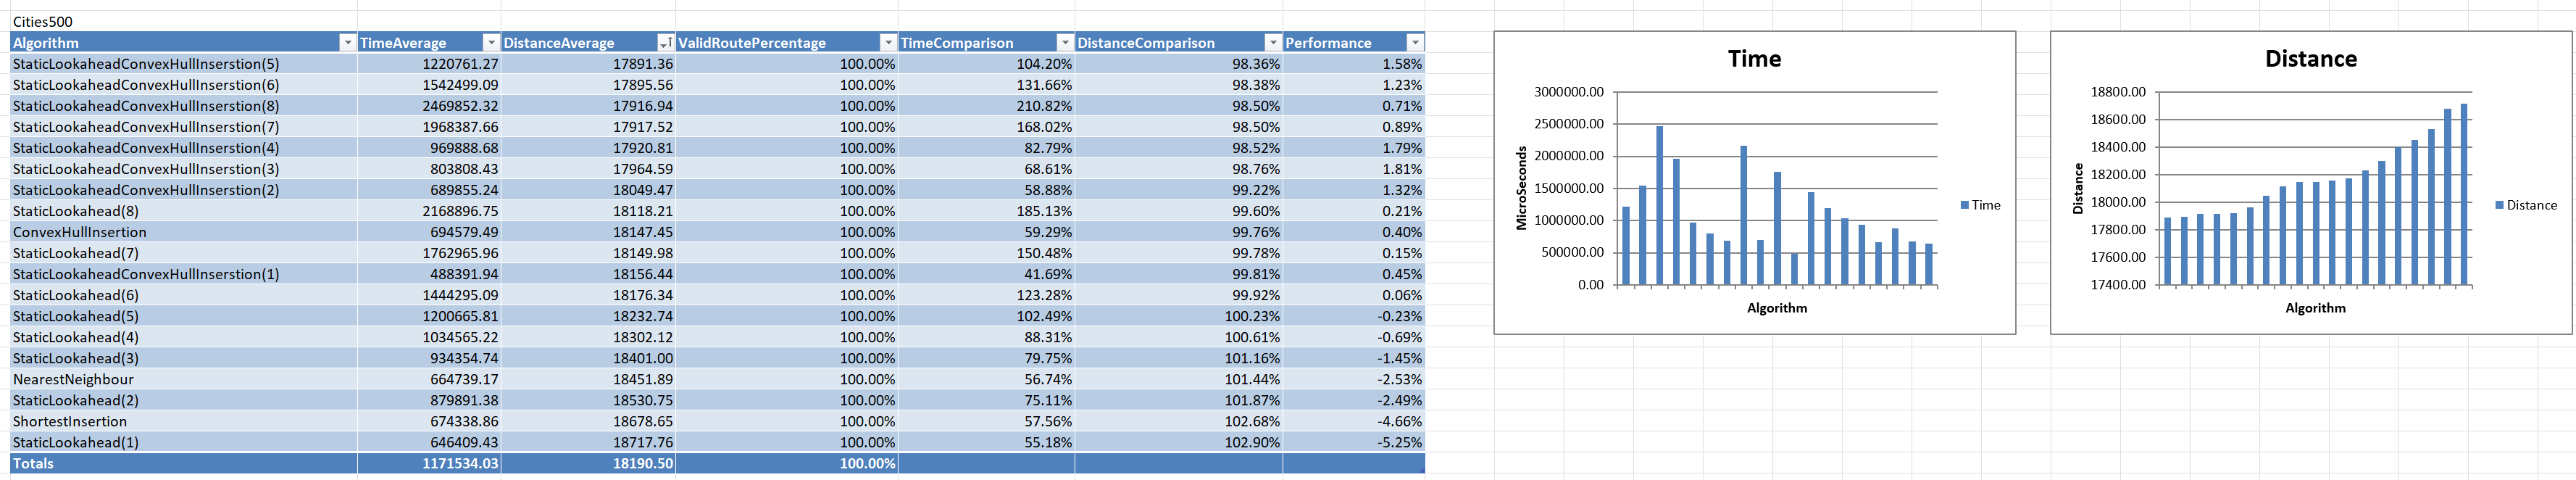
\includegraphics[width=\textwidth]{sections/image/excelfile.png}
    \caption{Excel File - Based On Size}
    \label{Excel1}
\end{figure}
\begin{figure}[H]
    \centering
    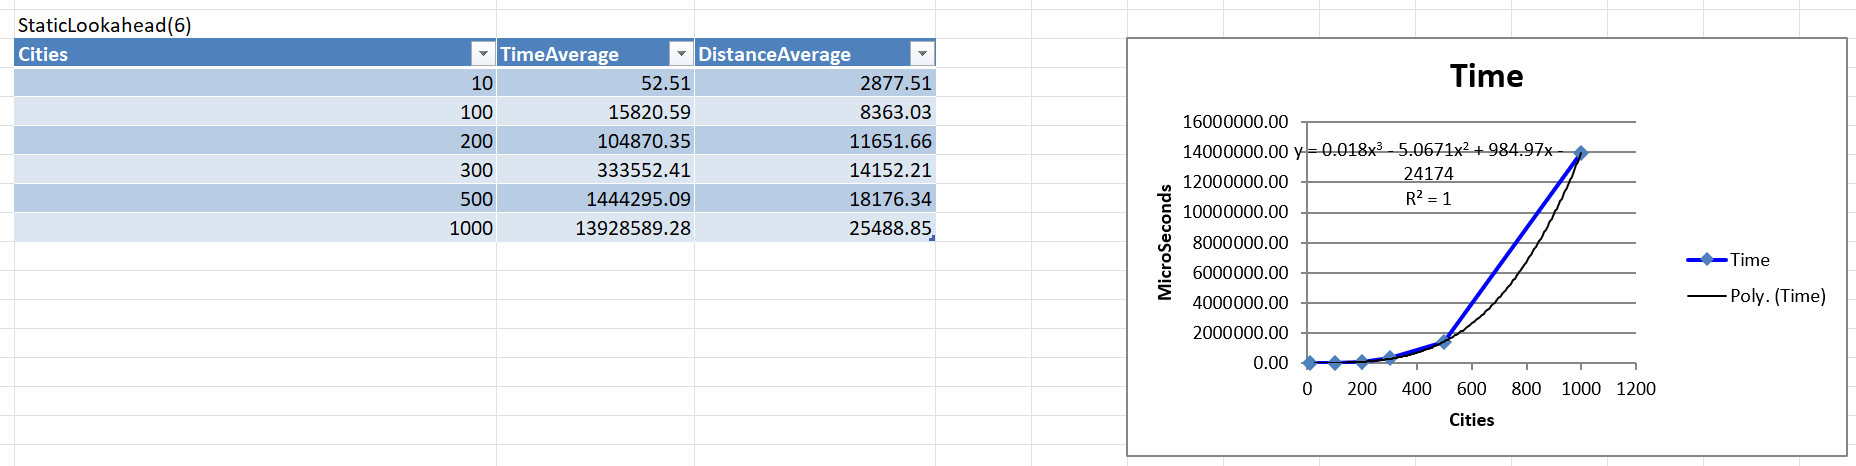
\includegraphics[width=\textwidth]{sections/image/ExcelFile2.png}
    \caption{Excel File - Based On Algorithm}
    \label{Excel2}
\end{figure}

\begin{center}
\section{Implementation}
\label{Implementation}
\end{center}

The code for this project was source-controlled using \href{https://github.com/}{GitHub}, and the repository can be found at \url{https://github.com/AndrewF001/Dissertation}. The concepts mentioned in the system requirement(Section\ref{sec:c++}), can be applied to the design of the system(Section\ref{design}), and were implemented multiple times throughout the project. A few principal elements from the code have been selected to highlight the concepts used and key features. Nevertheless, due to the complexity and large volume of code, not every advanced technique could be demonstrated.

\subsection{Polymorphism}

For the Testing Suites class(Figure\ref{fig:Emprical}), polymorphism ensures common functionality between test suites. Essential data is encapsulated between the classes, and pure virtual functions are defined to allow child classes to have individual functionality. Listing\ref{code:testing} is a stripped-down version of the code in \href{https://github.com/AndrewF001/Dissertation/blob/main/TSP_Solution/Empirical_Testing/Tests/test_class.h}{test\_class.h}. $TestClass$ is the pure virtual abstract parent class, and $RunTests()$ is the interface code for the GUI application. The interface code is split into public($RunTests()$) and private($\_test()$) functions, as the interface relies upon threads($std::packaged\_task$). Class $BasicTest$ is the child class of $TestClass$ and overrides the pure virtual function $Test()$ with the test suite definition(Table\ref{tab:testsuites}). 

{\hyphenpenalty=50\exhyphenpenalty=50
\begin{lstlisting}[caption={Testing Suites Polymorphic Classes}, label={code:testing},numbers=left]
class TestClass
{
public:

	std::shared_ptr<TSPFile> RunTests(size_t num_of_ittr = SIZE_MAX, std::chrono::seconds timeout = std::chrono::seconds::max()) {
            // package task to cancel if it takes too long
            std::packaged_task<void()> task(std::bind(&TestClass::_test, this, num_of_ittr));
    
            // Wait for the task to finish or timeout
            if (future.wait_for(timeout) != std::future_status::timeout) {
                // Task was successfully completed
                thr.join();
                future.get();
            }
            return m_file;
	}

private:
	void _test(size_t num_of_ittr) {
    		size_t i = 0;
    		while (i < num_of_ittr) {
    			Test();  // Uses Virtual Function
    			i++;
    		}
	}
	
	virtual void Test() = 0;   // Virtual Function
};

class BasicTest : public TestClass {
public:
	void Test() override { // Override Function
            // Control
            auto seed = Tester::seed_gen();
            auto cities = Tester::generateCities<Size>(seed);
            TSPArgs args;
    
            m_tester.TestAlgorithm<Size, ConstructionType::ConvexHullInsertion, Opt>(seed, cities, args);
            m_tester.TestAlgorithm<Size, ConstructionType::NearestNeighbour, Opt>(seed, cities, args);
            m_tester.TestAlgorithm<Size, ConstructionType::ShortestInsertion ,Opt>(seed, cities, args);
            m_tester.TestAlgmorithm<Size, ConstructionType::DynamicLookahead, Opt>(seed, cities, args);
            m_tester.TestAlgorithm<Size, ConstructionType::DynamicLookaheadConvexHullInserstion, Opt>(seed, cities, args);
    
            for (size_t i = 1; i < 9; i++) {
                args.max_depth = i;
                m_tester.TestAlgorithm<Size, ConstructionType::StaticLookahead, Opt>(seed, cities, args);
                m_tester.TestAlgorithm<Size, ConstructionType::StaticLookaheadConvexHullInserstion, Opt>(seed, cities, args);
            }
	};
};
\end{lstlisting}
}

\subsection{Template Metaprogramming}

Template Metaprogramming(TMP)(Section\ref{template}) is a valuable tool for performance optimisation and compile-time polymorphism. One of the optimisations used in the program is to turn builder classes into monolithic classes if the type is known at compile time; this is how TSP\_Library is implemented and can be found in \href{https://github.com/AndrewF001/Dissertation/blob/main/TSP_Solution/TSP_Library/tsp_template.h}{tsp\_template.h}. Using Enums and $constexpr$ If statements, the choice selection of a child class can be decided at compile-time with compile-time polymorphism. Listing\ref{code:template}, an edited snippet of code from \href{https://github.com/AndrewF001/Dissertation/blob/main/TSP_Solution/TSP_Library/tsp_template.h}{tsp\_template.h}; looks at how this compile-time polymorphism is applied to $constructTour()$ with the use of $ConstructionType$ Enum and $Construction$ template variable. By assigning the template variable to the Enum values(Line12) and modifying the builder function($constructTour()$, Line24) to the creation of predefined children classes, the use of a V-Table is avoided. As templates are instantiated for each template variable(Section\ref{template}), there are 96 different versions of the $TspTemplate$ being compiled, but adding more algorithms increases the number rapidly:

{\hyphenpenalty=50\exhyphenpenalty=50

\begin{equation*}
  \begin{aligned}
    \text{\# of template instantiation} &=C\cdot O\cdot CT\cdot PT\cdot T\\
    96 &=8\cdot 2\cdot 3\cdot 2\cdot 1
  \end{aligned}
\end{equation*}
Where: $C$ is the number of $ConstructionType$, $O$ is the number of $OptimisationType$, $CT$ is the number of $CachingType$, $PT$ is the number of $PartitioningType$, $T$ is the number of $TSPType$.

\begin{lstlisting}[caption={TSP Library Template Meta-Programming}, label={code:template},numbers=left]
enum class ConstructionType {
	DynamicLookahead,
	DynamicLookaheadConvexHullInserstion,
	StaticLookaheadConvexHullInserstion,
	StaticLookahead,
	NearestNeighbour,
	ShortestInsertion,
	ConvexHullInsertion,
	ConvexHull,
};

template <class TSPType, size_t Size, CachingType Caching, PartitioningType Partitioning, ConstructionType Construction, OptimisationType Optimisation>
class TspTemplate {
public:
    void run(const TSPArgs& args) {
    	m_data.initalisePartition();
    	m_data.initaliseCache();
    	constructTour(args);
    	optimiseTour(args);
    	finaliseOutput();
    };

private:
    void constructTour(const TSPArgs& args) {
    	if constexpr (Construction == ConstructionType::StaticLookaheadConvexHullInserstion)
    		StaticLookaheadConvexHull<TSPType, Size, Caching, Partitioning>(args.max_depth).constructTour(m_data);
    
            ... Multiple If Statements for all the values of ConstructionType ...
    
    	if constexpr (Construction == ConstructionType::DynamicLookaheadConvexHullInserstion)
    		DynamicLookaheadConvexHull<TSPType, Size, Caching, Partitioning>(args.max_depth, args.dynamic_args).constructTour(m_data);    		
    };
};
\end{lstlisting}
}
\subsection{API}

APIs are used everywhere but are mostly used in-depth by \href{https://github.com/AndrewF001/Dissertation/blob/main/TSP_Solution/TSP_Library/tsp_data/tsp_data_template.h}{TSP\_Data}. It is the central block that contains the Travelling Salesman Problem data and abides by its constraints. It also manages the interoperability of all the blocks and ensures software engineering optimisation is enforced. TSP\_Data has many public functions(Section\ref{tspData} \& Figure\ref{fig:TSP_Data}), but Listing\ref{code:Interface} looks at how caching(Section\ref{lit:Caching}) is managed for fetching the distance of an edge. Obscuring the caching mechanism behind an API call also requires that $m\_cities$(Line24) cannot be accessed from outside the class, potentially letting other classes bypass the caching mechanism.

\begin{lstlisting}[caption={TSP Data Interface}, label={code:Interface},numbers=left]
class TspDataTemplate {
public:
    double getDistance(cityID city1, cityID city2) {
        if constexpr (Caching == CachingType::full)
    		return m_cache[city1][city2];
    
        double result;
        if constexpr (Caching == CachingType::partial) {
            result = m_cache[city1][city2];
            // Check if the value is already in the cache
            if (result != DBL_MAX)						
                return result;
        }

        // Calculate the distance and store result
        result = m_cities[city1].getDistance(m_cities[city2]);	
        if constexpr (Caching == CachingType::partial)
            m_cache[city1][city2] = result;
    
        return result;
    };

private:
    std::array<TSPType, Size> m_cities;		// Array of cities
};
\end{lstlisting}

\pagebreak
\begin{landscape}

\subsection{Static Look-Ahead Cheapest Insertion Heuristic}

The development and implementation of SLACIH(Section\ref{SLACIH}) is the project's main focus, and its implementation serves as the proof of work. As described above, it builds upon polymorphism, templates, and API calls to remain adaptable and optimised. It incorporates all the optimisations used by the other algorithms but also includes several unique algorithmic optimisation techniques:
\begin{itemize}
    \item Early exit if the current distance exceeds the best-known solution(Line88)
    \item Use of closeness proximity(Section\ref{partitioning}) by only considering points within the distance of the current best solution(Line62)
    \item Early exit if no points are within range of a partial\_route(Line83).
\end{itemize}

Listing\ref{code:SLACIH} shows the complete, mostly unedited, C++ code of the algorithm, which can also be found in \href{https://github.com/AndrewF001/Dissertation/blob/main/TSP_Solution/TSP_Library/tour_construction/static_lookahead.h}{static\_lookahead.h}.

%The development and implementation of SLACIH(Section\ref{SLACIH}) is the main research of the project, and its implementation is the proof of work. It builds upon the polymorphism, templates, and API calls shown above to be adaptable and optimised. It uses all the optimisation as the other algorithms but has a few unique algorithmic optimisation techniques: early exit if the current distance is over the current best solution(Line88), using closeness proximity(Section\ref{partitioning}) by only considering points within distance of current best solution(Line62), and early exit if no points are within range of a $partail\_route$(Line83). Listing\ref{code:SLACIH} shows the complete, mostly unedited, C++ code of the algorithm, which can also be found in \href{https://github.com/AndrewF001/Dissertation/blob/main/TSP_Solution/TSP_Library/tour_construction/static_lookahead.h}{static\_lookahead.h}.
{\hyphenpenalty=50\exhyphenpenalty=50
\begin{lstlisting}[caption={Static Look-Ahead Cheapest Insertion Heuristic}, label={code:SLACIH},numbers=left]
template<class TSPType, size_t Size, CachingType Caching, PartitioningType Partitioning>
class StaticLookahead : public ConstructionBase<TSPType, Size, Caching, Partitioning>
public:
void _constructTour(TspDataTemplate& data) override {
    data.setCityPos(0, 0);	// Randomly select the first city
    lookaheadInsertion(data, m_depth);
};

static void lookaheadInsertion(TspDataTemplate& data, size_t depth) {
    const size_t additions = Size - data.getRouteSize();
    for (size_t i = 0; i < additions; i++) {
        auto [closest_point, route_position] = FindClosestPoints(data, depth);
        data.setCityPos(closest_point, route_position + 1);
    }
}

static std::pair<cityID, size_t> FindClosestPoints(TspDataTemplate& data, size_t depth) {
    double min_dist = DBL_MAX;
    std::pair<cityID, size_t> output;

    // Check if depth is greater than the number of cities left
    if (Size - data.getRouteSize() < depth)
        depth = Size - data.getRouteSize();
    // Check each city
    for (cityID idx = 0; idx < Size; idx++) {
        if (data.isCityInRoute(idx)) 
            continue; // If in route continue	

        // Find the shortest partital route for the city
        auto [distance, position] = ShortestRoute(data, idx, depth, min_dist);
        if (distance < min_dist) {
            min_dist = distance;
            output = { idx, position };
        }
    }
    return output;
}
private:
const size_t m_depth;
static std::pair<double, cityID> ShortestRoute(TspDataTemplate& data, cityID point, size_t depth, const double best_distance) {
    std::pair<double, cityID> output = { DBL_MAX, SIZE_MAX };	// distance, position
    std::vector<cityID> partail_route(3);
    partail_route[1] = point;
    
    // find the best place to insert the point
    const auto& route = data.getRoute();
    for (size_t i = 0; i < data.getRouteSize(); i++) {
        double distance = data.calcDeivation(partail_route[1], data.getRouteCityID(route[i]), data.getRouteCityID(route[i + 1]));
        if (distance < output.first) {
            output.first = distance;
            output.second = i;
        }
    }
    // Add it to partail route
    partail_route[0] = data.getRouteCityID(route[output.second]);
    partail_route[2] = data.getRouteCityID(route[output.second + 1]);
    // Repeat for lookaheads
    // Find closest point that is a part of partial route
    double offset = best_distance * best_distance;
    std::vector<cityID> city_search = data.getCitiesInArea(partail_route[1], offset);

    for (size_t i = 0; i < depth - 1; i++) {
        double min_dist = DBL_MAX;
        std::pair<cityID, size_t> add_point = { SIZE_MAX, SIZE_MAX };
        for (const auto& city : city_search) {
            if (data.isCityInRoute(city))
                continue;
            // Check if point is already in partail route
            if (std::any_of(partail_route.begin() + 1, partail_route.end() - 1, [city](const auto& route_point) { return route_point == city; }))
                continue;

            for (size_t j = 0; j < partail_route.size() - 1; j++) {
                double distance = data.calcDeivation(city, partail_route[j], partail_route[j + 1]);
                if (distance < min_dist) {
                    min_dist = distance;
                    add_point = { city, j };
                }
            }
        }
        if (add_point.first == SIZE_MAX)	// No point found
            break;
        // add closest point to partail route
        partail_route.insert(partail_route.begin() + add_point.second + 1, add_point.first);
        output.first += min_dist;
        if (output.first > best_distance)
            break;
    }
    return output;
}
};
\end{lstlisting}
}
\end{landscape}
\subsection{Dynamic Look-Ahead Cheapest Insertion Heuristic}

DLACIH expands on SLACIH with a optimal depth function(Listing\ref{code:DLACIH}), afterwards it is unchanged from the base algorithm. The cost function is defined in Equation\ref{depth_form}, which can be seen in Function $optimalDepth()$(line7) with the arguments being determined by the struct $DynamicArgs$.
{\hyphenpenalty=50\exhyphenpenalty=50
\begin{lstlisting}[caption={Dynamic Look-Ahead Cheapest Insertion Heuristic Depth Function}, label={code:DLACIH},numbers=left]
struct DynamicArgs {	// Numbers are from Gradient Descent analysis
	double multiplier = 1.2348586676954691;
	double logrithm = 0.90649189814814557;
	double constant = -1.6065204475308614;
};

static size_t optimalDepth(size_t size, size_t max_depth, DynamicArgs& args) {
    size_t optimal = (size_t)std::round(args.multiplier * std::log(args.logrithm * size) - args.constant);
    
    if (optimal == 0)
        optimal = 1;
    
    return std::min(optimal, max_depth);
}
\end{lstlisting}
}

\subsection{Gradient Descent}

Gradient descent is a useful tool for optimising the depth function arguments with empirical data as the cost function is convex. To obtain better results that are not hyper-optimised, taking the summation of a set of problems is beneficial, as displayed by Listing\ref{code:graident} where the $NumOfProblems=5$(Line1). How the gradient descent is set up can be seen in \href{https://github.com/AndrewF001/Dissertation/blob/main/TSP_Solution/Empirical_Testing/Tests/dynamic_args_gradient_descent.h}{dynamic\_args\_gradient\_descent.h}.
{\hyphenpenalty=50\exhyphenpenalty=50
\begin{lstlisting}[caption={Graident Descent Cost Function}, label={code:graident},numbers=left]
NumOfProblems = 5;
double cost_function(const gsl_vector* v, void* params) {
    double score = 0;
    std::array<std::unique_ptr<std::array<Type2d, Size>>, NUMOFPROBLEMS>* m_cities = (std::array<std::unique_ptr<std::array<Type2d, Size>>, NUMOFPROBLEMS>*)params;
    
    DynamicArgs d_args = { .multiplier = gsl_vector_get(v, 0), .logrithm = gsl_vector_get(v, 1), .constant = gsl_vector_get(v, 2) };
    
    TSPArgs args{ .max_depth = 10, .timeout_ms = std::chrono::milliseconds(300000), .dynamic_args = d_args};

    for (size_t i = 0; i < NUMOFPROBLEMS; i++) {
        auto algorithm = std::make_unique<TspTemplate<Type2d, Size, CachingType::full, PartitioningType::quadTree, ConstructionType::DynamicLookaheadConvexHullInserstion, OptimisationType::TwoOpt>>(AREA, *((*m_cities)[i]), GenerationType::rectangle, 0);
        score += algorithm->run(args).final_distance;
    }
    return score;
}
\end{lstlisting}
}
\begin{center}
\section{Project Management}
\label{waterfall}
\end{center}

Before the official project start date, a feasibility study was conducted, including the creation of a simple prototype over the 2024 summer break to validate the algorithm. In doing so, it highlighted opportunities for future work and areas of improvement. The work conducted could not be transferred to the main project, as an entire redesign of the system was necessary with the addition of TSP\_Data and the project's planned features.

At the start of the project, a proposed timeline defining the development of major features was produced(Figure\ref{fig:timeline}). Key milestones were identified that needed to be reached before moving on, as each system was built on top of the other. This led to the natural conclusion of using the waterfall project management model\cite{thesing2021agile}, requiring each step to design, implement, and test the current feature. This process ensured that backtracking or refactoring was not needed as the trust in existing code for future development was guaranteed.

\begin{figure}[H]
    \centering
    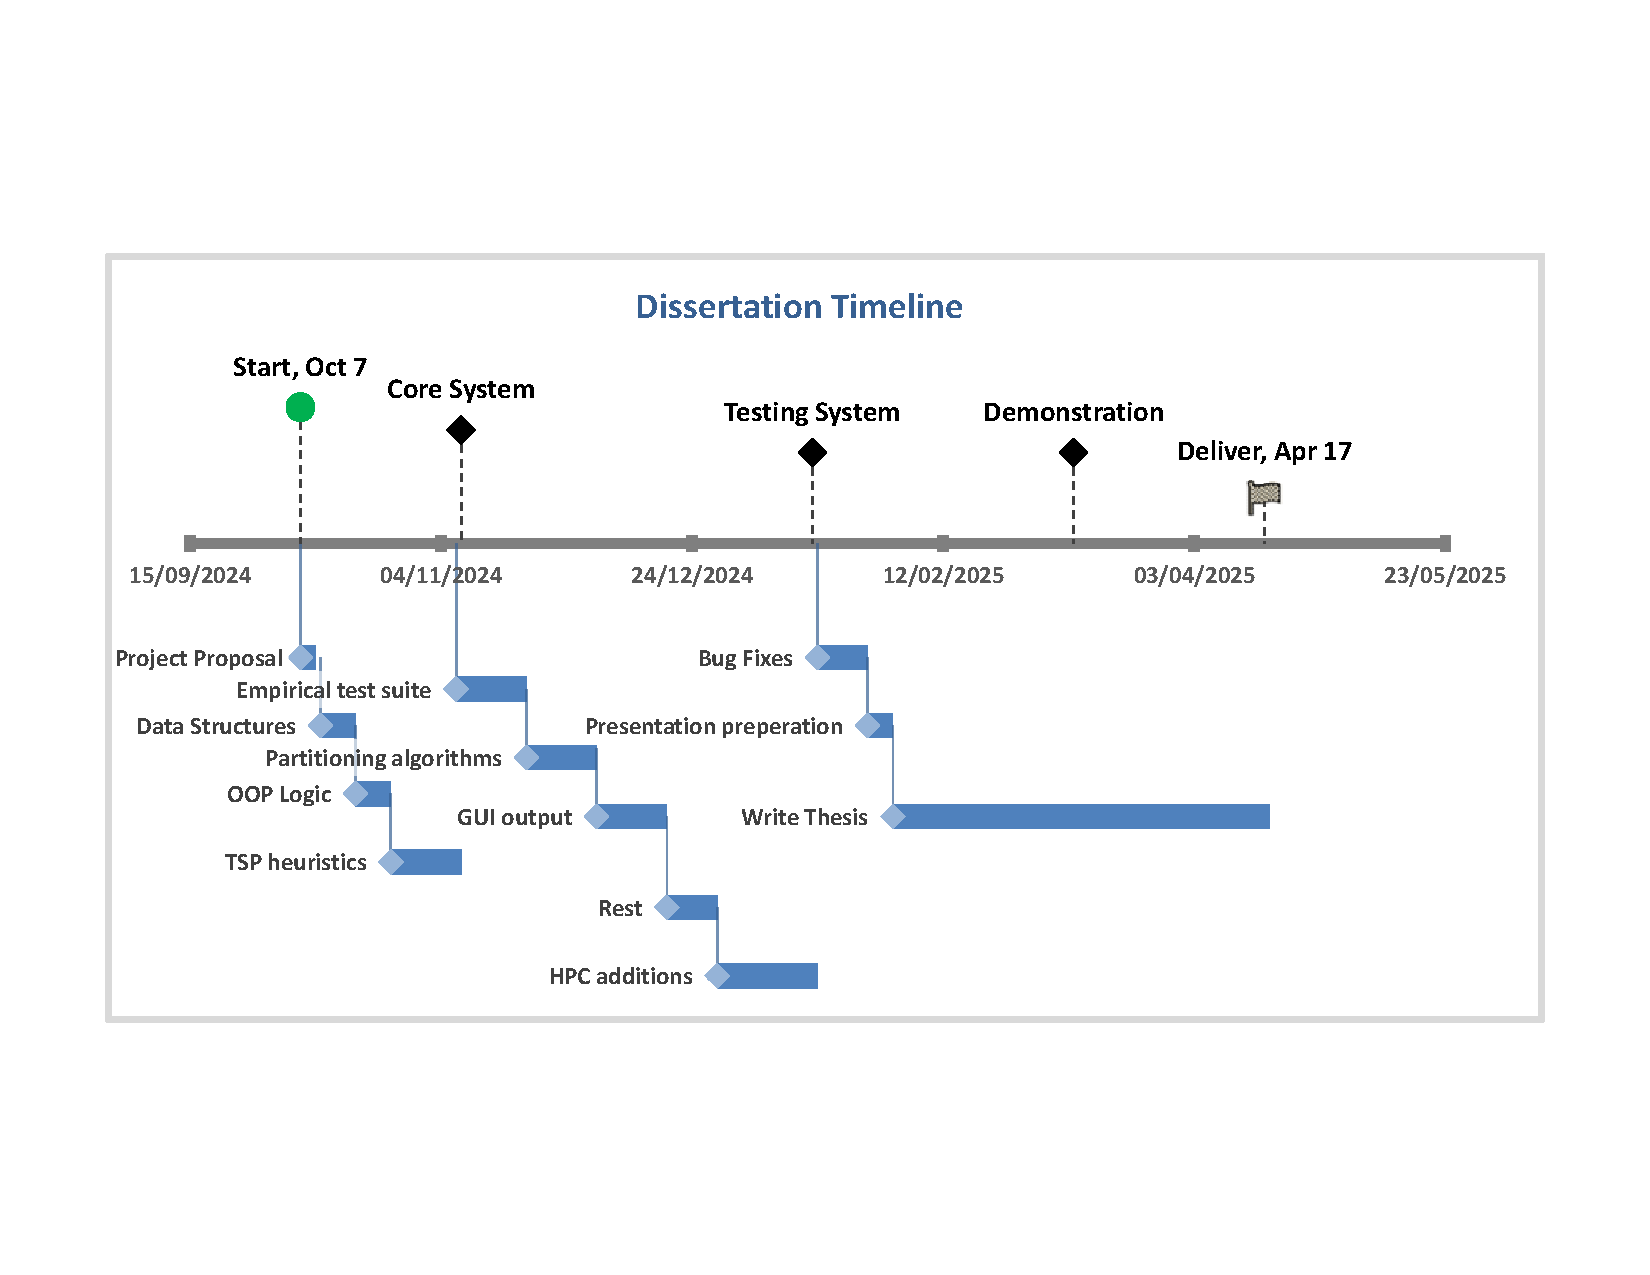
\includegraphics[width=0.9\textwidth]{sections/image/timeline.pdf}
    \caption{Project Timeline}
    \label{fig:timeline}
\end{figure}

The major milestones split the project between the core system(TSP Library) and application-specific development. Both of the major milestones had minor milestones that structured the development process of each system(Figure\ref{fig:timeline}). Similar to many projects, the project overran due to ambitious goals, leading to the high-performance computing feature being removed from the project scope in order to meet the final delivery date. Nonetheless, the quality of work and development efficiency achieved throughout the project were the highest delivered.
\begin{center}
\section{Unit Testing}
\label{sec:unittesting}
\end{center}

Unit Testing is part of the waterfall development cycle(Section\ref{waterfall}) to ensure current components function as intended. The tests should follow the design principles(Section\ref{designUnit}) of keeping it simple with one independent variable for testing. GoogleTest\cite{googletest} was used as the testing framework, but it functions the same as most testing frameworks. The tests should focus on the smallest components possible to provide the greatest coverage across the system. The testing uses a result-driven approach by using $asserts()$ on the value produced against the expected value, providing long-standing coverage if the code unexpectedly changes behaviour.

\subsection{Basic Types}

The basic types such as point, edge, and square are used throughout the program and therefore should be robust. They are tested on creation and on each of their functions with boundary testing. Listing\ref{code:point} shows the unit testing of $Point2D$ class constructor and $gradient()$ function against predetermined values calculated manually.

\begin{lstlisting}[caption={Point Unit Test},numbers=left,label={code:point}]
TEST(PointTest, Creation) {
	Point2D p1{ 0, 0 };
	EXPECT_EQ(p1.m_x, 0);
	EXPECT_EQ(p1.m_y, 0);

	Point2D p2{ 10, 10 };
	EXPECT_EQ(p2.m_x, 10);
	EXPECT_EQ(p2.m_y, 10);
}

TEST(PointTest, Gradient) {
	Point2D p1{ 0, 0 };
	Point2D p2{ 10, 10 };
	Point2D p3{ 10, 0 };
	Point2D p4{ 0, 10 };
	Point2D p5{ -10, -10 };

	EXPECT_EQ(p1.gradient(p2), 1);	// Positive slope
	EXPECT_EQ(p1.gradient(p5), 1);	// Same slop reverse position
	EXPECT_EQ(p1.gradient(p3), 0);  // Horizontal line
	EXPECT_EQ(p1.gradient(p4), INFINITY); // Virtical line
}
\end{lstlisting}

\subsection{Quad Tree}

The partitioning algorithms have more sophisticated functionality, with more complex data structures, which rely on the basic data types to function. Exhaustive boundary testing cannot be applied because there is a non-finite number of Quad Tree structures, but testing the sub-procedure can guarantee each step. Listing\ref{code:quad} shows the creation, insertion, and searching of a basic quad-tree to test its subdividing properties.

\begin{lstlisting}[caption={Quad tree Unit Test},numbers=left,label={code:quad}]
TEST(QuadTreeTest, BasicSearch) {
	QuadTree tree(Square{ {0, 0}, 100, 100 });
	tree.insert(0, Point2D{ 60, 60 }); // Root
	tree.insert(1, Point2D{ 30, 30 }); // Top left
	tree.insert(2, Point2D{ 70, 70 }); // Bottom right
	tree.insert(3, Point2D{ 30, 70 }); // Bottom left
	tree.insert(4, Point2D{ 70, 30 }); // Top right

	auto found = tree.contains(Square{ {0, 0}, 40, 40 });
	check_result(found, { 1 });
}
\end{lstlisting}

\subsection{Look-Ahead Algorithm}

Testing a look-ahead algorithm is infeasible as it requires doing a dry run of the algorithm manually. There are also too many parameters to cover all test cases exhaustively. Therefore, applying Stability Tests to ensure the code remains the same between versions and does not crash is acceptable. Listing\ref{code:looktest} confirms that the class compiles and runs without crashing for example data.


{\hyphenpenalty=50\exhyphenpenalty=50
\begin{lstlisting}[caption={SLACIH Stability Test},numbers=left,label={code:looktest}]
TEST(StaticLookahead, Similarity) {
	Square area = { {0, 0}, 1000, 1000 };
	std::mt19937 engine(1);

	auto cities = TspDataTemplate<Type2d, 50, CachingType::full, PartitioningType::quadTree>::generateCities(area, GenerationType::rectangle, engine);

	auto lookahead = std::make_unique<TspTemplate<Type2d, 50, CachingType::full, PartitioningType::linearSearch, ConstructionType::StaticLookaheadConvexHullInserstion, OptimisationType::None>>(area, cities)->run({1});
	auto linear = std::make_unique<TspTemplate<Type2d, 50, CachingType::full, PartitioningType::linearSearch, ConstructionType::ConvexHullInsertion, OptimisationType::None>>(area, cities)->run({});

	EXPECT_EQ(lookahead.route, linear.route);
}
\end{lstlisting}
}

\subsection{JSON Conversion}

Testing on the JSON conversion code helps protect against file corruption. As the conversion is symmetric, round case testing can be used to compare the written and read data. Listing\ref{code:JSON} demonstrates the symmetrically properties by comparing the original object with the round case object to determine they are identical. 

\begin{lstlisting}[caption={Json Round Case Test},numbers=left, label={code:JSON}]
TEST(JsonConversionTest, RunModeTest) {
	RunMode s; // Original value
	s.num_cities = 10;
	s.genType = GenerationType::rectangle;
	s.Caching = CachingType::full;
	s.Partitioning = PartitioningType::quadTree;
	s.Construction = ConstructionType::StaticLookaheadConvexHullInserstion;
	s.Optimisation = OptimisationType::TwoOpt;
	s.args = { 1, 2, std::chrono::milliseconds(100) };

	rapidjson::Document doc;
	doc.SetObject();
	rapidjson::Value val;
	jsonconversion::runModeToJson(s, val, doc.GetAllocator()); // Write JSON
	doc.AddMember("runMode", val, doc.GetAllocator());
	RunMode r;
	jsonconversion::JsonToRunMode(r, doc["runMode"]);  // Read JSON

	EXPECT_EQ(s.num_cities, r.num_cities); // Round case testing
	EXPECT_EQ(s.genType, r.genType);
	EXPECT_EQ(s.Caching, r.Caching);
	EXPECT_EQ(s.Partitioning, r.Partitioning);
	EXPECT_EQ(s.Construction, r.Construction);
	EXPECT_EQ(s.Optimisation, r.Optimisation);
	EXPECT_EQ(s.args, r.args);
}
\end{lstlisting}

%\subsection{CI/CD}
%I need to do this
\begin{center}
\section{Evaluation}
\label{sec:eval}
\end{center}

The project can be evaluated on its software engineering achievement(Section\ref{sec:system}) and the proposed SLACIH and DLACIH algorithm performance(Section\ref{method}); each has its challenges, with clear goals and strategies outlined. The evaluation in this section has been backed up with evidence of data in achieving the goals.

\subsection{Functional \& Non-Functional Requirements}

For the software engineering achievements, precise requirements were set in the functional and non-functional requirements(Section\ref{sec:requirements}). 
 The requirements in Table\ref{tab:functionalreq}\&\ref{tab:nonfunctionalreq} have been evaluated with what has been achieved in the Tables\ref{tab:functionalachieved}\&\ref{tab:nonfunctionalachieved}: 

\begin{table}[H]
    \centering
    \renewcommand{\arraystretch}{1.2} % Adjust row height for readability
    \begin{tabularx}{\textwidth}{|p{4cm}|X|}
\hline
\multicolumn{1}{|c|}{{\ul \textbf{Requirement}}} & \multicolumn{1}{c|}{{\ul \textbf{Achieved}}} \\ \hline
1.a) Graph Theory                              &  Two-dimensional graphs are represented in \href{https://github.com/AndrewF001/Dissertation/blob/main/TSP_Solution/TSP_Library/tsp_data/types/2d.h}{2d.h} and tested     \\ \hline
1.b) TSP Constraints                           &  \href{https://github.com/AndrewF001/Dissertation/blob/main/TSP_Solution/TSP_Library/tsp_data/tsp_data_template.h}{tsp\_data\_template.h} correctly enforces the constraints of the Travelling Salesman Problem     \\ \hline
1.c) Euclidean TSP                             &  The $getDistance()$ function correctly calculates the Euclidean distance  \\ \hline
 \makecell[l]{2.a) Facilities for \\ Algorithms}                  &  \href{https://github.com/AndrewF001/Dissertation/blob/main/TSP_Solution/TSP_Library/tsp_template.h}{tsp\_template.h} allows multiple algorithms to be used simply by changing a variable value   \\ \hline
 \makecell[l]{2.b) Benchmarking \\ Algorithm}                     &   \href{https://github.com/AndrewF001/Dissertation/blob/main/TSP_Solution/Utilities/timer.h}{timer.h} is a custom-built high-resolution clock timer specifically built for this project, and extended \href{https://github.com/AndrewF001/Dissertation/blob/main/TSP_Solution/TSP_Library/file_handling/tsp_structs.h}{tsp\_file} to include all the information needed\\ \hline
2.c) Algorithm Fairness                        &   The use of compile-time polymorphism treats every algorithm as individual sets of code, each being inlined and optimised by the compiler without knowledge of the other algorithm, and each algorithm worked with the same API calls and features\\ \hline
2.d) Testing Suite                             &  There are 5 test suites(Table\ref{tab:testsuites}), and developed on a \href{https://github.com/AndrewF001/Dissertation/blob/main/TSP_Solution/Empirical_Testing/Tests/test_class.h}{stable testing platform}                                          \\ \hline
 \makecell[l]{3.a) Display TSP \\ Solutions}                     &  There is a GUI application for displaying one or many TSP solutions \\ \hline
4.a) Collect Test Data                         &  TSP files with test data are created in JSON format \\ \hline
4.b) Analysis Test Data                        &  Excel tables and graphs and programmatically produced from the TSP files   \\ \hline
5.a) Unit Test                                 &  The unit tests covers TSP\_Library but not all aspects all aspects of the code base  \\ \hline
    \end{tabularx}
    \caption{Functional Requirements Achieved}
    \label{tab:functionalachieved}
\end{table}

\begin{table}[H]
    \centering
    \renewcommand{\arraystretch}{1.2} % Adjust row height for readability
    \begin{tabularx}{\textwidth}{|X|X|}
    \hline
{\ul \textbf{Requirement}}                                                                         & {\ul \textbf{Achieved}} \\ \hline
The user should be able to select the type of algorithm they want easily                   & The user can efficiently run pre-made algorithm setups, however, because compile-time polymorphism requires knowledge of which algorithm will be run beforehand, unless the user is a programmer, they are unlikely able to configure the bespoke algorithm            \\ \hline
The program should never fail or crash                                                     & The testing suites were run for multiple days without a crash or invalid TSP solution          \\ \hline
The program should be responsive and utilise all computing power                           & The program does not hang and uses all available cores when running multiple solutions         \\ \hline
The program should be adaptable and fill the needs of each executable                      & There is no repeated code to cover the same functionality       \\ \hline
The GUI should be easy to read for all users e.g. inclusive of those with colour blindness &      The colour palette does not clash with common colour blindness, but the graphics are small and lack graphical fidelity features like anti-aliasing             \\ \hline
    \end{tabularx}
    \caption{Non-Functional Requirements Achieved}
    \label{tab:nonfunctionalachieved}
\end{table}
\pagebreak
\subsection{Empirical Testing Results}

Following this report's research, methodology, design and testing; empirical testing is the lead evaluation for comparing the Static \& Dynamic Look-Ahead Cheapest Insertion Heuristic against other known heuristics. Every algorithm(Table\ref{tab:algacry}) used Quad-Tree Partitioning, Full Caching, and tour optimiser with 2-opt swap, because from testing this was shown to be the best set-up for solution result and run time.

\begin{table}[H]
    \centering
    \renewcommand{\arraystretch}{1.2} % Adjust row height for readability
    \begin{tabularx}{\textwidth}{|p{2.5cm}|X|}
    \hline
      \textbf{Acronym}   & \textbf{Algorithm} \\
      \hline
        DLACHCIH & Dynamic Look-Ahead Convex Hull Cheapest Insertion Heuristic\\
        DLACIH & Dynamic Look-Ahead Cheapest Insertion Heuristic \\
        SLACHCIH(X) & Static Look-Ahead Convex Hull Cheapest Insertion Heuristic, Depth = X\\
        SLACIH(X) & Static Look-Ahead Cheapest Insertion Heuristic, Depth = X \\
        NNS & Nearest Neighbour Search Heuristic \\
        CHCIH & Convex Hull Cheapest Insertion Heuristic \\
        CIH & Cheapest Insertion Heuristic \\
        \hline
    \end{tabularx}
    \caption{Algorithm Acronym Key}
    \label{tab:algacry}
\end{table}

Each test instance problem was randomly generated. and ran on each algorithm for six problem sizes, which were chosen to represent small, medium, and large problems. Multiple depths of the static look-ahead were evaluated to prove and develop the dynamic look-ahead optimal depth curvature. \label{test:dynamic}This report theorised lots of dynamic algorithms(Section\ref{Dynamic}), but for this testing, only static dynamic depth optimisation(Section\ref{SDynamic}) was considered. As DLACIH calls upon SLACIH code and therefore would generate the same solution, running the code twice was avoided to speed up testing. The distance values for DLACIH and DLACHCIH are based on the static depth it would have chosen to run SLACIH, and the times can be assumed to be identical, but left blank for clarity.

Each value in the Table\ref{tab:DistanceResult}\&\ref{tab:TimeResult} is the mean average of 1,000 problems being solved. This results in 114,000 TSP problems being solved and 240,540,000 Nodes being routed. This required multiple weeks of constant computational running and tens of thousands of CPU hours.

\begin{landscape}
% \pagebreak
% \begin{table}
%   \centering
%   \setlength\tabcolsep{0pt}
%   \begin{tabular*}{\linewidth}{@{\extracolsep{\fill}}
%                         |p{3cm}|
%                    *{2}{S[table-format= 1.5]}|
%                    *{2}{S[table-format= 1.5]}|
%                    *{2}{S[table-format= 1.5]}|
%                    *{2}{S[table-format= 1.5]}|
%                    *{2}{S[table-format= 1.5]}|
%                    *{2}{S[table-format= 1.5]}|
%                             } 
%     \toprule 
    
%      & \multicolumn{12}{c}{\textbf{Problem Size}}\\
%      &   \multicolumn{2}{c}{10 Nodes}   &   \multicolumn{2}{c}{100 Nodes}  &\multicolumn{2}{c}{200 Nodes}  &\multicolumn{2}{c}{300 Nodes}  &\multicolumn{2}{c}{500 Nodes}  &\multicolumn{2}{c}{1000 Nodes}   \\
%     \midrule
%     {\textbf{Algorithm}}&   {\thead[b]{Distance}} &   {\thead[b]{Time}}
%     &   {\thead[b]{Distance}} &   {\thead[b]{Time}}
%     &   {\thead[b]{Distance}} &   {\thead[b]{Time}}
%     &   {\thead[b]{Distance}} &   {\thead[b]{Time}}
%     &   {\thead[b]{Distance}} &   {\thead[b]{Time}}
%     &   {\thead[b]{Distance}} &   {\thead[b]{Time}}\\
%     \midrule
% {DLACHCIH}       & {0.123}    & {1.234} & {0.12}     & {0.123}    & {0.123} & {0.123} & {1.234} & {1.234} & {1.234} & {1.234} & {1.234} & {1.234}        \\ 
% \myrowcolour%
% {DLACIH}         & {0.123}    & {1.234} & {0.12}     & {0.123}    & {0.123} & {0.123} & {1.234} & {1.234} & {1.234} & {1.234} & {1.234} & {1.234}        \\ 
% {SLACHCIH(0)} & {2864.35} & {28.83} & {8191.25} & {5051.86} & {11490.84} & {36190.85} & {14062.30} & {111427.81} & {18156.44} & {488391.94} & {25651.97} & {3620307.70} \\
% \myrowcolour%
% {SLACHCIH(1)} & {2864.57} & {25.37} & {8151.50} & {7261.49} & {11433.55} & {48326.42} & {13988.46} & {155657.94} & {18049.47} & {689855.24} & {25467.84} & {6353401.04} \\
% {SLACHCIH(2)} & {2864.46} & {24.09} & {8140.39} & {8234.30} & {11398.91} & {56582.62} & {13939.97} & {182868.75} & {17964.59} & {803808.43} & {25327.55} & {7537333.35} \\
% \myrowcolour%
% {SLACHCIH(3)} & {2864.55} & {24.06} & {8138.31} & {10040.87} & {11396.14} & {69633.18} & {13908.57} & {218068.36} & {17920.81} & {969888.68} & {25256.85} & {9223702.34} \\
% {SLACHCIH(4)} & {2864.47} & {24.41} & {8143.77} & {12184.33} & {11385.62} & {87280.23} & {13900.00} & {272952.20} & {17891.36} & {1220761.27} & {25210.99} & {11632562.85} \\
% \myrowcolour%
% {SLACHCIH(5)} & {2864.45} & {24.44} & {8150.61} & {14956.88} & {11394.39} & {108331.81} & {13902.06} & {343997.62} & {17895.56} & {1542499.09} & {25180.95} & {14895643.66} \\
% {SLACHCIH(6)} & {2864.45} & {24.71} & {8162.80} & {17467.33} & {11398.80} & {134173.32} & {13906.92} & {432163.16} & {17917.52} & {1968387.66} & {25177.56} & {19003165.87} \\
% \myrowcolour%
% {SLACHCIH(7)} & {2864.45} & {24.18} & {8173.54} & {20843.73} & {11418.06} & {164704.99} & {13933.31} & {533267.40} & {17916.94} & {2469852.32} & {25184.09} & {23702107.36} \\
% {SLACIH(0)} & {2898.15} & {39.98} & {8620.55} & {7902.99} & {11990.80} & {52819.91} & {14581.91} & {155816.52} & {18717.76} & {646409.43} & {26242.28} & {4608439.04} \\
% \myrowcolour%
% {SLACIH(1)} & {2886.81} & {43.13} & {8540.03} & {9994.76} & {11885.12} & {65427.01} & {14441.23} & {205581.55} & {18530.75} & {879891.38} & {25998.57} & {7931265.55} \\
% {SLACIH(2)} & {2885.52} & {42.97} & {8480.63} & {10616.85} & {11783.13} & {68674.72} & {14343.36} & {216557.75} & {18401.00} & {934354.74} & {25802.91} & {8607775.94} \\
% \myrowcolour%
% {SLACIH(3)} & {2878.55} & {45.30} & {8420.75} & {11922.03} & {11721.57} & {76106.33} & {14256.36} & {238098.60} & {18302.12} & {1034565.22} & {25658.64} & {9749928.92} \\
% {SLACIH(4)} & {2878.31} & {49.89} & {8373.10} & {13914.21} & {11685.38} & {88204.19} & {14199.79} & {271463.36} & {18232.74} & {1200665.81} & {25545.87} & {11465799.93} \\
% \myrowcolour%
% {SLACIH(5)} & {2877.51} & {52.51} & {8363.03} & {15820.59} & {11651.66} & {104870.35} & {14152.21} & {333552.41} & {18176.34} & {1444295.09} & {25488.85} & {13928589.28} \\
% {SLACIH(6)} & {2874.40} & {59.00} & {8343.51} & {19406.64} & {11628.51} & {127248.89} & {14132.63} & {394223.06} & {18149.98} & {1762965.96} & {25436.01} & {17155433.92} \\
% \myrowcolour%
% {SLACIH(7)} & {2873.75} & {58.87} & {8336.78} & {22896.07} & {11605.18} & {154385.62} & {14121.65} & {479555.42} & {18118.21} & {2168896.75} & {25419.93} & {21146002.81} \\
% {NNS} & {2888.89} & {51.85} & {8494.45} & {8163.56} & {11828.17} & {53758.76} & {14379.98} & {160573.75} & {18451.89} & {664739.17} & {25847.28} & {4624162.49} \\
% \myrowcolour%
% {CHCIH} & {2864.35} & {74.79} & {8190.42} & {16037.53} & {11492.43} & {61741.36} & {14063.86} & {173547.76} & {18147.45} & {694579.49} & {25581.89} & {4909795.79} \\
% {CIH} & {2898.15} & {39.75} & {8619.66} & {7892.48} & {11991.10} & {53696.50} & {14571.81} & {158542.26} & {18678.65} & {674338.86} & {26132.84} & {4904754.48} \\
%  \bottomrule
%   \end{tabular*}
%   \begin{tablenotes}[flushleft]\small
%   \source: Average of 1000 random problems
%   \note:   Red values are best in class
%   \end{tablenotes}
%   \caption{Empirical Testing Results }\label{tab:results2}
% \end{table}

{\captionsetup{font=Large, labelsep=space}
% \begin{table}
%   \centering
%   \caption{Empirical Testing Distance Results }\label{tab:DistanceResult}
%   \setlength\tabcolsep{0pt}
%   \begin{tabular*}{\linewidth}{@{\extracolsep{\fill}}
%                 |p{3cm}|p{3cm}|p{3cm}|p{3cm}|p{3cm}|p{3cm}|p{3cm}|
%                    % *{6}{S[table-format= 1.5]}|
%                             } 
%     \toprule 
%      & \multicolumn{5}{c}{\textbf{Problem Size}} \\
%      \cmidrule[0.4pt](r{0.125em}){2-7}%
%      {\textbf{Algorithm}} &  {10 Nodes}   &  {100 Nodes}  & {200 Nodes}  & {300 Nodes}  & {500 Nodes}  & {1000 Nodes}   \\
%     \midrule

% \ DLACHCIH & \highest{2864.35} & \highest{8138.31} & \highest{11385.62} & 13902.06 & 17895.56 & 25180.95 \\
% \myrowcolour
% \ DLACIH & 2898.15 & 8420.75 & 11685.38 & 14256.36 & 18176.34 & 25436.01 \\
% \ SLACHCIH(0) & \highest{2864.35} & 8191.25 & 11490.84 & 14062.30 & 18156.44 & 25651.97 \\
% \myrowcolour
% \ SLACHCIH(1) & 2864.57 & 8151.50 & 11433.55 & 13988.46 & 18049.47 & 25467.84 \\
% \ SLACHCIH(2) & 2864.46 & 8140.39 & 11398.91 & 13939.97 & 17964.59 & 25327.55 \\
% \myrowcolour
% \ SLACHCIH(3) & 2864.55 & \highest{8138.31} & 11396.14 & 13908.57 & 17920.81 & 25256.85 \\
% \ SLACHCIH(4) & 2864.47 & 8143.77 & \highest{11385.62} & \highest{13900.00} & \highest{17891.36} & 25210.99 \\
% \myrowcolour
% \ SLACHCIH(5) & 2864.45 & 8150.61 & 11394.39 & 13902.06 & 17895.56 & 25180.95 \\
% \ SLACHCIH(6) & 2864.45 & 8162.80 & 11398.80 & 13906.92 & 17917.52 & \highest{25177.56} \\
% \myrowcolour
% \ SLACHCIH(7) & 2864.45 & 8173.54 & 11418.06 & 13933.31 & 17916.94 & 25184.09 \\
% \ SLACIH(0)  & 2898.15 & 8620.55 & 11990.80 & 14581.91 & 18717.76 & 26242.28 \\
% \myrowcolour
% \ SLACIH(1)  & 2886.81 & 8540.03 & 11885.12 & 14441.23 & 18530.75 & 25998.57 \\
% \ SLACIH(2)  & 2885.52 & 8480.63 & 11783.13 & 14343.36 & 18401.00 & 25802.91 \\
% \myrowcolour
% \ SLACIH(3)  & 2878.55 & 8420.75 & 11721.57 & 14256.36 & 18302.12 & 25658.64 \\
% \ SLACIH(4)  & 2878.31 & 8373.10 & 11685.38 & 14199.79 & 18232.74 & 25545.87 \\
% \myrowcolour
% \ SLACIH(5)  & 2877.51 & 8363.03 & 11651.66 & 14152.21 & 18176.34 & 25488.85 \\
%  \scalebox{0.85}{ SLACIH(6)  & 2874.40 & 8343.51 & 11628.51 & 14132.63 & 18149.98 & 25436.01 \\
% \myrowcolour
% \ SLACIH(7)  & 2873.75 & 8336.78 & 11605.18 & 14121.65 & 18118.21 & 25419.93 \\
% \ NNS         & 2888.89 & 8494.45 & 11828.17 & 14379.98 & 18451.89 & 25847.28 \\
% \myrowcolour
% \ CHCIH       & 2864.35 & 8190.42 & 11492.43 & 14063.86 & 18147.45 & 25581.89 \\
% \ CIH         & 2898.15 & 8619.66 & 11991.10 & 14571.81 & 18678.65 & 26132.84 \\
%  \bottomrule
%   \end{tabular*}
%   \begin{tablenotes}[flushleft]\small
%   \source: Average of 1000 random problems
%   \note:   Red values are best in class
%   \end{tablenotes}
% \end{table}

\begin{table}[]
  \centering
  \caption{\\ Empirical Testing Distance Results }\label{tab:DistanceResult}
\resizebox{0.9\linewidth}{!}{%
\begin{tabular}{|c|cccccc|}
\hline
                                     & \multicolumn{6}{c|}{\textbf{Problem Size}}                                                                                                                                                              \\ \cline{2-7} 
\multirow{-2}{*}{\textbf{Algorithm}} & \multicolumn{1}{l|}{10 Nodes}  & \multicolumn{1}{l|}{100 Nodes} & \multicolumn{1}{l|}{200 Nodes}  & \multicolumn{1}{l|}{300 Nodes}  & \multicolumn{1}{l|}{500 Nodes}  & \multicolumn{1}{l|}{1000 Nodes} \\ \hline
\textbf{DLACHCIH}                    & {\color[HTML]{FE0000} 2864.35} & {\color[HTML]{FE0000} 8138.31} & {\color[HTML]{FE0000} 11385.62} & 13902.06                        & 17895.56                        & 25180.95                        \\
\rowcolor[HTML]{EFEFEF} 
\textbf{DLACIH}                      & 2898.15                        & 8420.75                        & 11685.38                        & 14256.36                        & 18176.34                        & 25436.01                        \\
\textbf{SLACHCIH(0)}                 & {\color[HTML]{FE0000} 2864.35} & 8191.25                        & 11490.84                        & 14062.30                        & 18156.44                        & 25651.97                        \\
\rowcolor[HTML]{EFEFEF} 
\textbf{SLACHCIH(1)}                 & 2864.57                        & 8151.50                        & 11433.55                        & 13988.46                        & 18049.47                        & 25467.84                        \\
\textbf{SLACHCIH(2)}                 & 2864.46                        & 8140.39                        & 11398.91                        & 13939.97                        & 17964.59                        & 25327.55                        \\
\rowcolor[HTML]{EFEFEF} 
\textbf{SLACHCIH(3)}                 & 2864.55                        & {\color[HTML]{FE0000} 8138.31} & 11396.14                        & 13908.57                        & 17920.81                        & 25256.85                        \\
\textbf{SLACHCIH(4)}                 & 2864.47                        & 8143.77                        & {\color[HTML]{FE0000} 11385.62} & {\color[HTML]{FE0000} 13900.00} & {\color[HTML]{FE0000} 17891.36} & 25210.99                        \\
\rowcolor[HTML]{EFEFEF} 
\textbf{SLACHCIH(5)}                 & 2864.45                        & 8150.61                        & 11394.39                        & 13902.06                        & 17895.56                        & 25180.95                        \\
\textbf{SLACHCIH(6)}                 & 2864.45                        & 8162.80                        & 11398.80                        & 13906.92                        & 17917.52                        & {\color[HTML]{FE0000} 25177.56} \\
\rowcolor[HTML]{EFEFEF} 
\textbf{SLACHCIH(7)}                 & 2864.45                        & 8173.54                        & 11418.06                        & 13933.31                        & 17916.94                        & 25184.09                        \\
\textbf{SLACIH(0)}                   & 2898.15                        & 8620.55                        & 11990.80                        & 14581.91                        & 18717.76                        & 26242.28                        \\
\rowcolor[HTML]{EFEFEF} 
\textbf{SLACIH(1)}                   & 2886.81                        & 8540.03                        & 11885.12                        & 14441.23                        & 18530.75                        & 25998.57                        \\
\textbf{SLACIH(2)}                   & 2885.52                        & 8480.63                        & 11783.13                        & 14343.36                        & 18401.00                        & 25802.91                        \\
\rowcolor[HTML]{EFEFEF} 
\textbf{SLACIH(3)}                   & 2878.55                        & 8420.75                        & 11721.57                        & 14256.36                        & 18302.12                        & 25658.64                        \\
\textbf{SLACIH(4)}                   & 2878.31                        & 8373.10                        & 11685.38                        & 14199.79                        & 18232.74                        & 25545.87                        \\
\rowcolor[HTML]{EFEFEF} 
\textbf{SLACIH(5)}                   & 2877.51                        & 8363.03                        & 11651.66                        & 14152.21                        & 18176.34                        & 25488.85                        \\
\textbf{SLACIH(6)}                   & 2874.40                        & 8343.51                        & 11628.51                        & 14132.63                        & 18149.98                        & 25436.01                        \\
\rowcolor[HTML]{EFEFEF} 
\textbf{SLACIH(7)}                   & 2873.75                        & 8336.78                        & 11605.18                        & 14121.65                        & 18118.21                        & 25419.93                        \\
\textbf{NNS}                         & 2888.89                        & 8494.45                        & 11828.17                        & 14379.98                        & 18451.89                        & 25847.28                        \\
\rowcolor[HTML]{EFEFEF} 
\textbf{CHCIH}                       & 2864.35                        & 8190.42                        & 11492.43                        & 14063.86                        & 18147.45                        & 25581.89                        \\
\textbf{CIH}                         & 2898.15                        & 8619.66                        & 11991.10                        & 14571.81                        & 18678.65                        & 26132.84                        \\ \hline
\end{tabular}%
}
  \begin{tablenotes}[flushleft]\small
  \source: Average of 1000 random problems
  \note:   Red values are best in class
  \end{tablenotes}
\end{table}

\pagebreak
% \begin{table}
%   \centering
%   \caption{Empirical Testing Time(Microseconds) Results}\label{tab:TimeResult}
%   \setlength\tabcolsep{0pt}
%     \begin{tabular*}{\linewidth}{@{\extracolsep{\fill}}
%                 |p{3cm}|p{3cm}|p{3cm}|p{3cm}|p{3cm}|p{3cm}|p{3cm}|
%                    % *{6}{S[table-format= 1.5]}|
%                             } 
%     \toprule 
%      & \multicolumn{5}{c}{\textbf{Problem Size}} \\
%      \cmidrule[0.4pt](r{0.125em}){2-7}%
%      {\textbf{\ Algorithm}} &  {10 Nodes}   &  {100 Nodes}  & {200 Nodes}  & {300 Nodes}  & {500 Nodes}  & {1000 Nodes}   \\
%     \midrule

% \ DLACHCIH & N/A & N/A & N/A & N/A & N/A & N/A \\
% \myrowcolour
% \ DLACIH & N/A & N/A & N/A & N/A & N/A & N/A \\
% \ SLACHCIH(0) & 28.83 & 5051.86 & 36190.85 & 111427.81 & 488391.94 & 3620307.70 \\
% \myrowcolour
% \ SLACHCIH(1) & 25.37 & 7261.49 & 48326.42 & 155657.94 & 689855.24 & 6353401.04 \\
% \ SLACHCIH(2) & 24.09 & 8234.30 & 56582.62 & 182868.75 & 803808.43 & 7537333.35 \\
% \myrowcolour
% \ SLACHCIH(3) & 24.06 & 10040.87 & 69633.18 & 218068.36 & 969888.68 & 9223702.34 \\
% \ SLACHCIH(4) & 24.41 & 12184.33 & 87280.23 & 272952.20 & 1220761.27 & 11632562.85 \\
% \myrowcolour
% \ SLACHCIH(5) & 24.44 & 14956.88 & 108331.81 & 343997.62 & 1542499.09 & 14895643.66 \\
% \ SLACHCIH(6) & 24.71 & 17467.33 & 134173.32 & 432163.16 & 1968387.66 & 19003165.87 \\
% \myrowcolour
% \ SLACHCIH(7) & 24.18 & 20843.73 & 164704.99 & 533267.40 & 2469852.32 & 23702107.36 \\
% \ SLACIH(0)  & 39.98 & 7902.99 & 52819.91 & 155816.52 & 646409.43 & 4608439.04 \\
% \myrowcolour
% \ SLACIH(1)  & 43.13 & 9994.76 & 65427.01 & 205581.55 & 879891.38 & 7931265.55 \\
% \ SLACIH(2)  & 42.97 & 10616.85 & 68674.72 & 216557.75 & 934354.74 & 8607775.94 \\
% \myrowcolour
% \ SLACIH(3)  & 45.30 & 11922.03 & 76106.33 & 238098.60 & 1034565.22 & 9749928.92 \\
% \ SLACIH(4)  & 49.89 & 13914.21 & 88204.19 & 271463.36 & 1200665.81 & 11465799.93 \\
% \myrowcolour
% \ SLACIH(5)  & 52.51 & 15820.59 & 104870.35 & 333552.41 & 1444295.09 & 13928589.28 \\
% \ SLACIH(6)  & 59.00 & 19406.64 & 127248.89 & 394223.06 & 1762965.96 & 17155433.92 \\
% \myrowcolour
% \ SLACIH(7)  & 58.87 & 22896.07 & 154385.62 & 479555.42 & 2168896.75 & 21146002.81 \\
% \ NNS         & 51.85 & 8163.56 & 53758.76 & 160573.75 & 664739.17 & 4624162.49 \\
% \myrowcolour
% \ CHCIH       & 74.79 & 16037.53 & 61741.36 & 173547.76 & 694579.49 & 4909795.79 \\
% \ CIH         & 39.75 & 7892.48 & 53696.50 & 158542.26 & 674338.86 & 4904754.48 \\
%  \bottomrule
%   \end{tabular*}
%   \begin{tablenotes}[flushleft]\small
%   \source: Average of 1000 random problems
%   \end{tablenotes}
% \end{table}

% \pagebreak

\begin{table}[]
  \centering
  \caption{\\ Empirical Testing Time(Microseconds) Results}\label{tab:TimeResult}
\resizebox{0.9\linewidth}{!}{%
\begin{tabular}{|c|cccccc|}
\hline
                                     & \multicolumn{6}{c|}{\textbf{Problem Size}}                                                                                                                                                          \\ \cline{2-7} 
\multirow{-2}{*}{\textbf{Algorithm}} & \multicolumn{1}{l|}{10 Nodes} & \multicolumn{1}{l|}{100 Nodes} & \multicolumn{1}{l|}{200 Nodes} & \multicolumn{1}{l|}{300 Nodes} & \multicolumn{1}{l|}{500 Nodes} & \multicolumn{1}{l|}{1000 Nodes} \\ \hline
\textbf{DLACHCIH}                    & N/A                           & N/A                            & N/A                            & N/A                            & N/A                            & N/A                             \\
\rowcolor[HTML]{EFEFEF} 
\textbf{DLACIH}                      & N/A                           & N/A                            & N/A                            & N/A                            & N/A                            & N/A                             \\
\textbf{SLACHCIH(0)}                 & 28.83                         & 5051.86                        & 36190.85                       & 111427.81                      & 488391.94                      & 3620307.70                      \\
\rowcolor[HTML]{EFEFEF} 
\textbf{SLACHCIH(1)}                 & 25.37                         & 7261.49                        & 48326.42                       & 155657.94                      & 689855.24                      & 6353401.04                      \\
\textbf{SLACHCIH(2)}                 & 24.09                         & 8234.30                        & 56582.62                       & 182868.75                      & 803808.43                      & 7537333.35                      \\
\rowcolor[HTML]{EFEFEF} 
\textbf{SLACHCIH(3)}                 & 24.06                         & 10040.87                       & 69633.18                       & 218068.36                      & 969888.68                      & 9223702.34                      \\
\textbf{SLACHCIH(4)}                 & 24.41                         & 12184.33                       & 87280.23                       & 272952.20                      & 1220761.27                     & 11632562.85                     \\
\rowcolor[HTML]{EFEFEF} 
\textbf{SLACHCIH(5)}                 & 24.44                         & 14956.88                       & 108331.81                      & 343997.62                      & 1542499.09                     & 14895643.66                     \\
\textbf{SLACHCIH(6)}                 & 24.71                         & 17467.33                       & 134173.32                      & 432163.16                      & 1968387.66                     & 19003165.87                     \\
\rowcolor[HTML]{EFEFEF} 
\textbf{SLACHCIH(7)}                 & 24.18                         & 20843.73                       & 164704.99                      & 533267.40                      & 2469852.32                     & 23702107.36                     \\
\textbf{SLACIH(0)}                   & 39.98                         & 7902.99                        & 52819.91                       & 155816.52                      & 646409.43                      & 4608439.04                      \\
\rowcolor[HTML]{EFEFEF} 
\textbf{SLACIH(1)}                   & 43.13                         & 9994.76                        & 65427.01                       & 205581.55                      & 879891.38                      & 7931265.55                      \\
\textbf{SLACIH(2)}                   & 42.97                         & 10616.85                       & 68674.72                       & 216557.75                      & 934354.74                      & 8607775.94                      \\
\rowcolor[HTML]{EFEFEF} 
\textbf{SLACIH(3)}                   & 45.30                         & 11922.03                       & 76106.33                       & 238098.60                      & 1034565.22                     & 9749928.92                      \\
\textbf{SLACIH(4)}                   & 49.89                         & 13914.21                       & 88204.19                       & 271463.36                      & 1200665.81                     & 11465799.93                     \\
\rowcolor[HTML]{EFEFEF} 
\textbf{SLACIH(5)}                   & 52.51                         & 15820.59                       & 104870.35                      & 333552.41                      & 1444295.09                     & 13928589.28                     \\
\textbf{SLACIH(6)}                   & 59.00                         & 19406.64                       & 127248.89                      & 394223.06                      & 1762965.96                     & 17155433.92                     \\
\rowcolor[HTML]{EFEFEF} 
\textbf{SLACIH(7)}                   & 58.87                         & 22896.07                       & 154385.62                      & 479555.42                      & 2168896.75                     & 21146002.81                     \\
\textbf{NNS}                         & 51.85                         & 8163.56                        & 53758.76                       & 160573.75                      & 664739.17                      & 4624162.49                      \\
\rowcolor[HTML]{EFEFEF} 
\textbf{CHCIH}                       & 74.79                         & 16037.53                       & 61741.36                       & 173547.76                      & 694579.49                      & 4909795.79                      \\
\textbf{CIH}                         & 39.75                         & 7892.48                        & 53696.50                       & 158542.26                      & 674338.86                      & 4904754.48                      \\ \hline
\end{tabular}%
}
  \begin{tablenotes}[flushleft]\small
  \source: Average of 1000 random problems
  \end{tablenotes}
\end{table}
}
\pagebreak
\end{landscape}

For every problem size(Table\ref{tab:DistanceResult}), SLACHCIH provided the best solution from the algorithms tested, although the same depth was not used. As theorised, as the problem size increases, a higher look-ahead depth is optimal. This is where DLACHCIH's optimal depth function proved to be highly fit for purpose. However, the gradient descent variable optimisation failed to find the optimal curve that could otherwise be found through statistical analysis. The data also correctly demonstrated the theory that a higher depth is not always better. This is due to the pitfalls the look-ahead design introduces when it searches for nodes far away from a cluster(Section\ref{pitfall}).

From the conventional heuristic, CHCIH is the leading algorithm, but none could be better than DLACHCIH for any problem size. Using Equation\ref{eqt:resultcompar} to compare the solution results vs DLACHCIH in a Table\ref{tab:performance}: 
\begin{equation}
    \frac{\text{Conventional}_{Result}}{\text{DLACHCIH}_{Result}}-1
    \label{eqt:resultcompar}
\end{equation}


\begin{table}[H]
\caption{DLACHCIH vs Conventional Algorithm }\label{tab:performance}
\begin{tabular}{|l|llllll|l|}
\hline
\multirow{2}{*}{\textbf{\begin{tabular}[c]{@{}l@{}}Conventional\\ Algorithm\end{tabular}}} & \multicolumn{6}{c|}{\textbf{Problem Size}}                                                                                                                                                          \\ \cline{2-7} 
                                                                                           & \multicolumn{1}{c|}{10 Nodes} & \multicolumn{1}{c|}{100 Nodes} & \multicolumn{1}{c|}{200 Nodes} & \multicolumn{1}{c|}{300 Nodes} & \multicolumn{1}{c|}{500 Nodes} & \multicolumn{1}{c|}{1000 Nodes} \\ \hline
\textbf{NNS}                                                                               & 0.856\%                       & 4.376\%                        & 3.887\%                        & 3.438\%                        & 3.109\%                        & 2.646\%                         \\
\textbf{CHCIH}                                                                             & 0.000\%                       & 0.640\%                        & 0.937\%                        & 1.164\%                        & 1.408\%                        & 1.592\%                         \\
\textbf{CIH}                                                                               & 1.18\%                        & 5.914\%                        & 5.318\%                        & 4.818\%                        & 4.376\%                        & 3.780\%                         \\ \hline
\end{tabular}

  \begin{tablenotes}[flushleft]\small
  \note: For any value above 0\% DLACHCIH performs better   
  \end{tablenotes}
\end{table}


\subsection{TSPLib Results}

When testing the TSPLib exact solution, each problem had a unique size; therefore, DLACIH was used as it performs best for an extensive range of problems. This was the only algorithm tested, as trying to hyper-optimise the depth would not represent the proposed algorithm fairly, as this would introduce a new independent variable to the evaluation. Table\ref{tab:TSPLibResult} outlines the distance against the exact solution for the 56 smallest Euclidean TSPLIB problems, which is all that could be computed in a reasonable time:
\pagebreak
\begin{longtable}{|p{.20\textwidth}|p{.20\textwidth}|p{.20\textwidth}|p{.20\textwidth}|} 
\hline
{ \textbf{Problem}} & { \textbf{Exact Solution}} & { \textbf{DLACIH Solution}} & {\textbf{Difference From Exact(\%)}} \\ \hline
eil51 & 426 & 442.918 & 3.971\%  \\ \myrowcolour
eil76 & 538 & 588.222 & 9.335\%  \\ 
pr76 & 108159 & 109872 & 1.584\%  \\ \myrowcolour
rat99 & 1211 & 1284.34 & 6.056\%  \\ 
rd100 & 7910 & 8028.18 & 1.494\%  \\ \myrowcolour
eil101 & 629 & 688.237 & 9.418\%  \\
pr107 & 44303 & 46065.5 & 3.978\%  \\ \myrowcolour
pr124 & 59030 & 59931.4 & 1.527\%  \\ 
bier127 & 118282 & 121483 & 2.706\%  \\  \myrowcolour
pr136 & 96772 & 98678.4 & 1.97\%  \\ 
pr144 & 58537 & 63973.6 & 9.287\%  \\ \myrowcolour
pr152 & 73682 & 75735.9 & 2.788\%  \\ 
u159 & 42080 & 45610.3 & 8.389\%  \\ \myrowcolour
rat195 & 2323 & 2536.77 & 9.202\%  \\ 
d198 & 15780 & 16714.3 & 5.921\%  \\ \myrowcolour
tsp225 & 3916 & 4127.81 & 5.409\%  \\ 
ts225 & 126643 & 141079 & 11.399\%  \\ \myrowcolour
pr226 & 80369 & 82470 & 2.614\%  \\ 
gil262 & 2378 & 2531.35 & 6.449\%  \\ \myrowcolour
pr264 & 49135 & 52329.2 & 6.501\%  \\ 
a280 & 2579 & 2729.76 & 5.846\%  \\ \myrowcolour
pr299 & 48191 & 51572.4 & 7.017\%  \\ 
rd400 & 15281 & 16233 & 6.23\%  \\ \myrowcolour
fl417 & 11861 & 12273 & 3.474\%  \\ 
pr439 & 107217 & 116485 & 8.644\%  \\ \myrowcolour
pcb442 & 50778 & 54220.4 & 6.779\%  \\ 
d493 & 35002 & 37947.2 & 8.414\%  \\ \myrowcolour
u574 & 36905 & 39236.6 & 6.318\%  \\ 
rat575 & 6773 & 7502.05 & 10.764\%  \\ \myrowcolour
p654 & 34643 & 35466.9 & 2.378\%  \\ 
d657 & 48912 & 52769.7 & 7.887\%  \\ \myrowcolour
u724 & 41910 & 45781.4 & 9.237\%  \\ 
rat783 & 8806 & 9638.47 & 9.453\%  \\ \myrowcolour
pr1002 & 259045 & 284101 & 9.672\%  \\ 
u1060 & 224094 & 242810 & 8.352\%  \\ \myrowcolour
vm1084 & 239297 & 261821 & 9.413\%  \\ 
pcb1173 & 56892 & 62368 & 9.625\%  \\ \myrowcolour
d1291 & 50801 & 57963.3 & 14.099\%  \\ 
rl1304 & 252948 & 271365 & 7.281\%  \\ \myrowcolour
rl1323 & 270199 & 291955 & 8.052\%  \\ 
nrw1379 & 56638 & 61127.3 & 7.926\%  \\ \myrowcolour
fl1400 & 20127 & 21485.2 & 6.748\%  \\ 
u1432 & 152970 & 165038 & 7.889\%  \\ \myrowcolour
fl1577 & 22249 & 24216.5 & 8.843\%  \\ 
d1655 & 62128 & 68199.4 & 9.772\%  \\ \myrowcolour
vm1748 & 336556 & 370251 & 10.012\%  \\ 
u1817 & 57201 & 64190.6 & 12.219\%  \\ \myrowcolour
rl1889 & 316536 & 344067 & 8.698\%  \\ 
d2103 & 80450 & 83940.4 & 4.339\%  \\ \myrowcolour
u2152 & 64253 & 72821.7 & 13.336\%  \\ 
u2319 & 234256 & 247967 & 5.853\%  \\ \myrowcolour
pr2392 & 378032 & 421713 & 11.555\%  \\ 
pcb3038 & 137694 & 150113 & 9.019\%  \\ \myrowcolour
fl3795 & 28772 & 30407 & 5.683\%  \\ \hline
\textbf{Total} & 4642099 & 5013946.707 & 8.01\% \\ \hline 
\caption{TSPLib Result}
\label{tab:TSPLibResult}
\end{longtable}
Using the Equation\ref{ptsplib} to take the average of all the results evenly, the average percentage difference is $7.2345\%$ greater than the exact solution. This is a respectable result, but is insignificant to current benchmarking heuristics that are able to get within $0.5\%$ of the exact solution\cite{HELSGAUN2000106}.

\subsection{Time Analysis}

Evaluating the time complexity of an algorithm based on run time, especially when variables affect the time complexity, can be difficult. The theory for the algorithm design puts the time complexity at $O(n^5)$(Equation\ref{equ:statictime}). In reality, the time complexity is closer to $n^3$ for low depths, but would be $n^5$ when $depth = n$. When dividing the time by the growth(Table\ref{tab:Timegrowth}), $n$ \& $n^2$ continue to grow exponentially, $n^4$ \& $n^5$ steadily decrease, while $n^3$ remains steady, suggesting the time complexity is $O(n^3)$ when the depth is seven. This is backed up when generating trend lines for a line graph of time vs size(Figure\ref{fig:timevssize}), where $n^3$ is the dominant factor. While the timings for every algorithm are present in Table\ref{tab:TimeResult}, hesitation in comparing them is advised as the classical heuristics were not as meticulously optimised as SLACIH. 

\begin{table}[H]
\centering
\begin{tabular}{lllllll}
\rowcolor[HTML]{4F81BD} 
{\color[HTML]{FFFFFF} \textbf{Cities}} & {\color[HTML]{FFFFFF} \textbf{TimeAverage}} & {\color[HTML]{FFFFFF} \textbf{t/n}} & {\color[HTML]{FFFFFF} \textbf{t/n\textasciicircum{}2}} & {\color[HTML]{FFFFFF} \textbf{t/n\textasciicircum{}3}} & {\color[HTML]{FFFFFF} \textbf{t/n\textasciicircum{}4}} & {\color[HTML]{FFFFFF} \textbf{t/n\textasciicircum{}5}} \\
\rowcolor[HTML]{B8CCE4} 
10                                     & 24.18                                       & 2.4183                              & 0.24183                                                & 0.024183                                               & 0.002418                                               & 0.000242                                               \\
\rowcolor[HTML]{DCE6F1} 
100                                    & 20843.73                                    & 208.43727                           & 2.084373                                               & 0.020844                                               & 0.000208                                               & 2.08E-06                                               \\
\rowcolor[HTML]{B8CCE4} 
200                                    & 164704.99                                   & 823.52493                           & 4.117625                                               & 0.020588                                               & 0.000103                                               & 5.15E-07                                               \\
\rowcolor[HTML]{DCE6F1} 
300                                    & 533267.40                                   & 1777.55799                          & 5.925193                                               & 0.019751                                               & 6.58E-05                                               & 2.19E-07                                               \\
\rowcolor[HTML]{B8CCE4} 
500                                    & 2469852.32                                  & 4939.70464                          & 9.879409                                               & 0.019759                                               & 3.95E-05                                               & 7.9E-08                                                \\
\rowcolor[HTML]{DCE6F1} 
1000                                   & 23702107.36                                 & 23702.10736                         & 23.70211                                               & 0.023702                                               & 2.37E-05                                               & 2.37E-08                                              
\end{tabular}
\caption{SLACHCIH(7) Time Growth}
\label{tab:Timegrowth}
\end{table}

\begin{figure}[H]
    \centering
    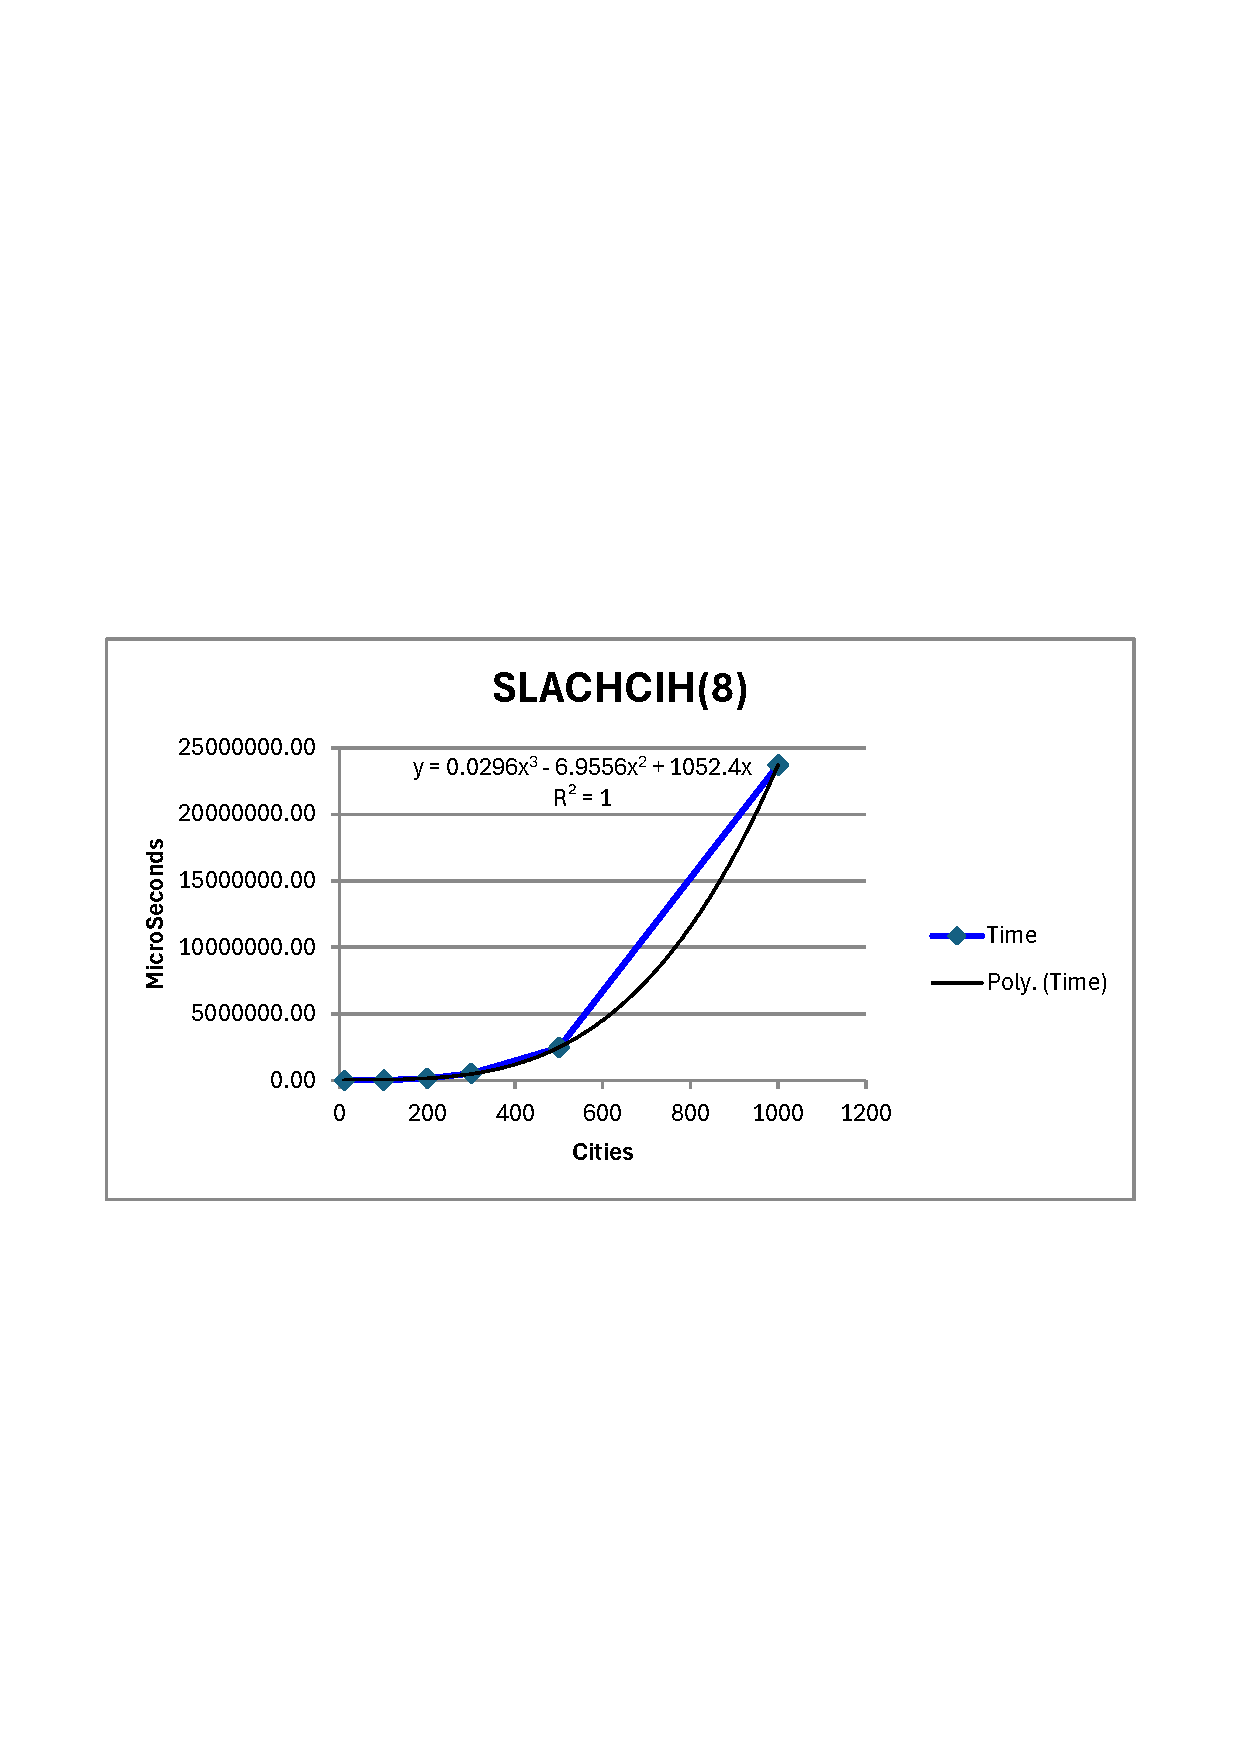
\includegraphics[width=0.8\textwidth]{sections/image/test_graph.pdf}
    \caption{SLACHCIH(8) Trend Line}
    \label{fig:timevssize}
\end{figure}

The value the look-ahead depth has is the difference between the algorithm time complexity being $O(n^3)$(when the depth is zero), and $O(n^5)$(when depth is $n$); this is the same as in Equation\ref{equ:statictime}. The CIH part of the algorithm is a constant $O(n^3)$ time complexity, while the look-ahead cost is based on the depth. This is observed in the data by changing the depths(Figure\ref{fig:timevsdepth}); the difference in time complexity is $O(n^2)$, which matches the cost of the look-ahead function.

The jump from depth zero to depth one is abrupt; this abnormally large increase is theorised as the cost of invoking the $ShortestRoute()$ function, which would only be fully invoked if depth is greater than 0. This is noticeable in Figure\ref{chart:depth} between the violet and indigo lines.
\begin{figure}[H]
    \centering
    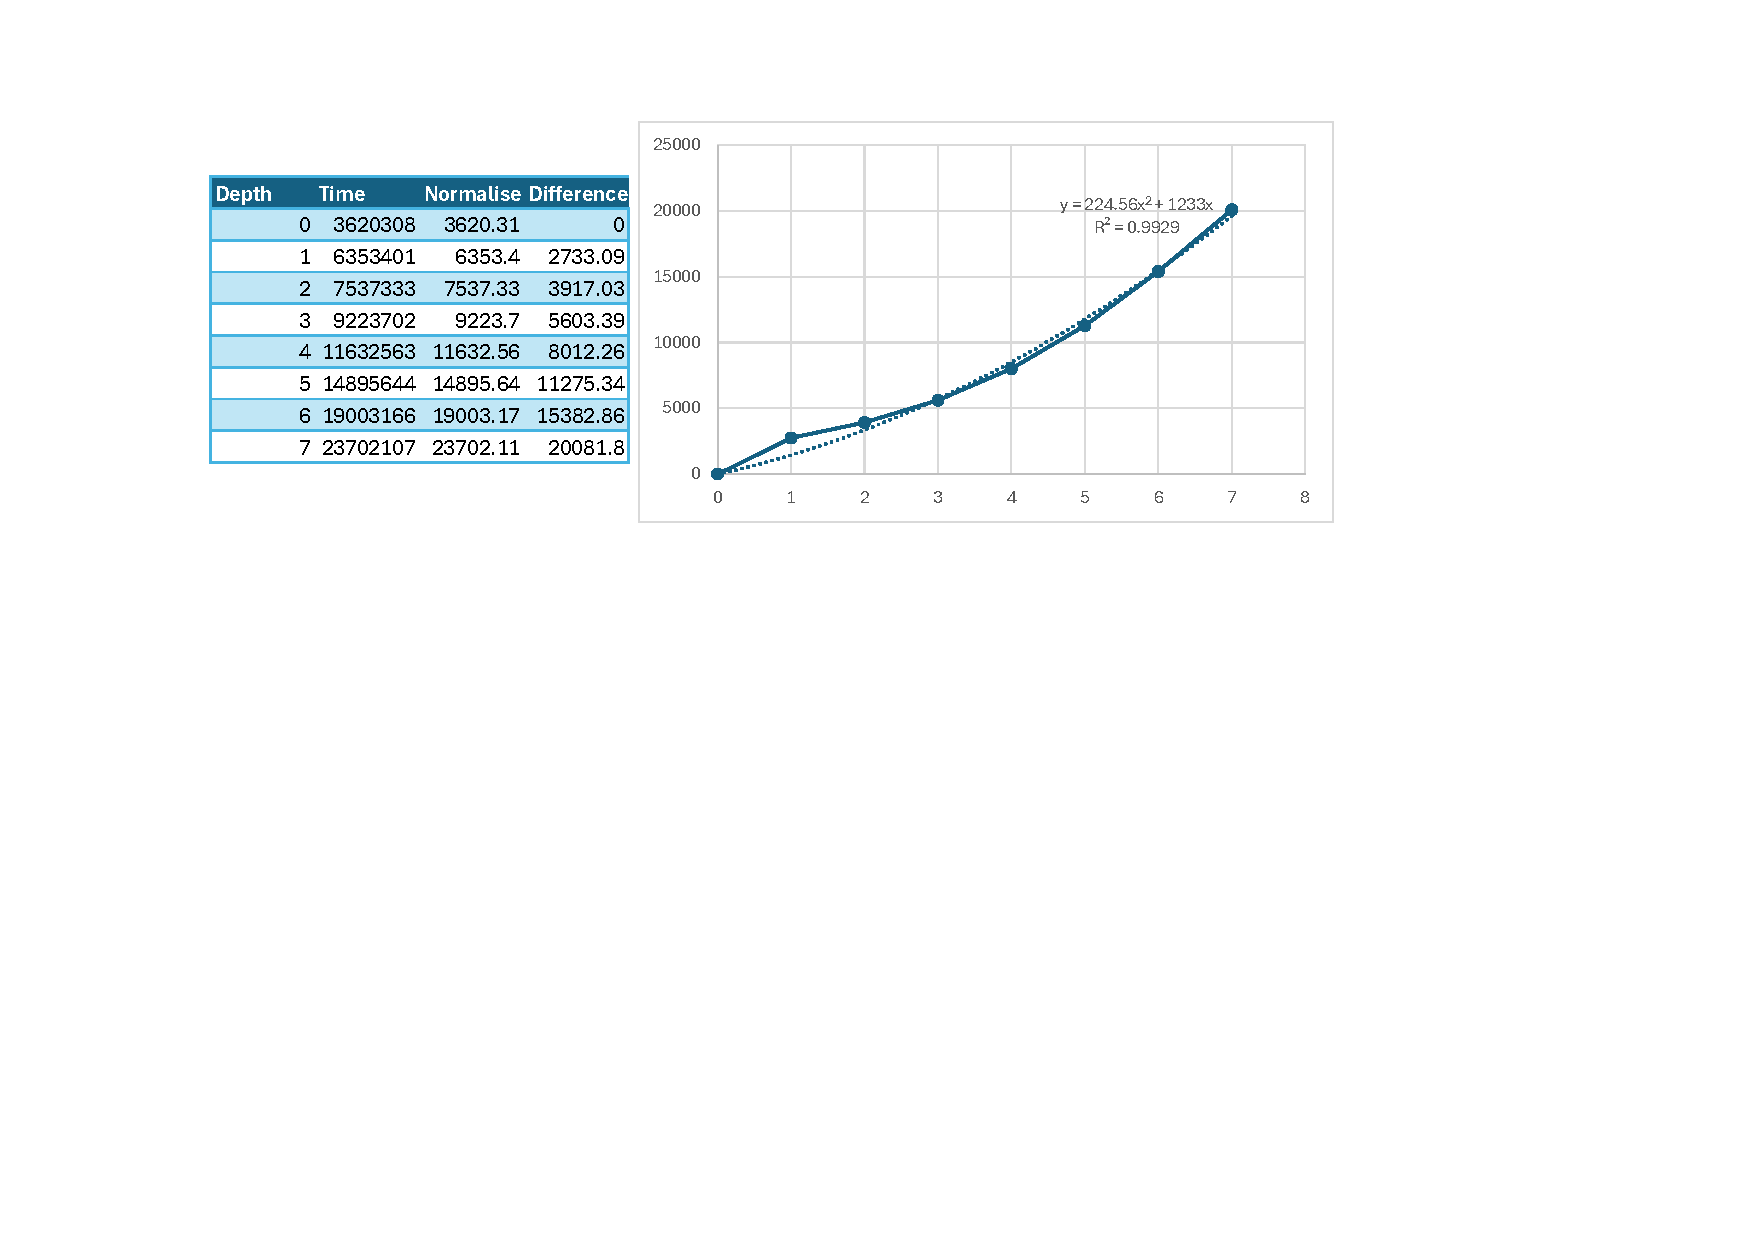
\includegraphics[width=\textwidth]{sections/image/test_graph2.pdf}
    \caption{Depth Trend Line}
    \label{fig:timevsdepth}
\end{figure}

\begin{figure}[H]
    \centering
    \resizebox{0.7\textwidth}{!}{%
    \begin{tikzpicture}
        \begin{axis}[
            xlabel={Problem Size}, 
            ylabel={MicroSeconds},
            title={Depth Vs Time},
            domain=1:1200, % Adjust range as needed
            samples=1000,
            grid=major,
            thick,
            legend style={at={(0.02,0.98)}, anchor=north west}, % Top-left corner
            legend entries={
                0 (Violet),
                1 (Indigo),
                2 (Blue),
                3 (Green),
                4 (Yellow),
                5 (Orange),
                6 (Red),
                7 (Black)
            }
        ]
    \addplot[violet] coordinates
      {(10,29) (100,5051) (200,36190) (300,111427) (500,488391)(1000,3620307)};

    \addplot[indigo] coordinates
      {(10,25.37) (100,7261.49) (200,48326.42) (300,155657.94) (500,689855.24)(1000,6353401.04)};

    \addplot[blue] coordinates
      {(10,24.09) (100,8234.30) (200,56582.62) (300,182868.75) (500,803808.43)(1000,7537333.35)};
      
      \addplot[green] coordinates
      {(10,24.06) (100,10040.87) (200,69633.18) (300,218068.36) (500,969888.68)(1000,9223702.34)};

      \addplot[yellow] coordinates
      {(10,24.41) (100,12184.33) (200,87280.23) (300,272952.20) (500,1220761.27)(1000,11632562.85)};
      
      \addplot[orange] coordinates
      {(10,24.44) (100,14956.88) (200,108331.81) (300,343997.62) (500,1542499.09)(1000,14895643.66)};

    \addplot[red] coordinates
      {(10,24.71) (100,17467.33) (200,134173.32) (300,432163.16) (500,1968387.66)(1000,19003165.87)};

      \addplot[black] coordinates
      {(10,24.18) (100,20843.73) (200,164704.99) (300,533267.40) (500,2469852.32)(1000,23702107.36)};


        \end{axis}
    \end{tikzpicture}
    }%
    \caption{Plot Of Depth Vs Time}
    \label{chart:depth}
\end{figure}
\begin{center}
\section{Conclusions}
\label{conc:aims}
\end{center}

Overall, this project has demonstrated that the Look-Ahead Cheapest Insertion Heuristic is a worthy heuristic in solving the Travelling Salesman Problem.

The project findings demonstrated consistent and significant gains in the solution result by applying a look-ahead design to the Cheapest Insertion Heuristic to avoid local pitfalls. A new algorithm, Dynamic Look-Ahead Convex Hull Cheapest Insertion Heuristic(DLACHCIH), produced a better result than conventional heuristics on average:

\begin{table}[H]
\centering
\begin{threeparttable}
\begin{tabular}{|l|l|}
\hline
\rowcolor[HTML]{EFEFEF} 
\textbf{Algorithm}                       & \textbf{Performance Difference} \\ \hline
Convex Hull Cheapest Insertion Heuristic & 1.1482\%                        \\ \hline
Cheapest Insertion Heuristic             & 4.8412\%                        \\ \hline
Nearest Neighbour Search                 & 3.4912\%                        \\ \hline
\end{tabular}
\begin{tablenotes}[flushleft]
\small
\item \textit{Note:} higher \% is better
\end{tablenotes}
\caption{Performance Of DLACHCIH vs Conventional Heuristics}
\end{threeparttable}
\end{table}

In the research of TSP, any gains are a great accomplishment to theorists, and the difference is better than expected. It proved the project motivation that a look-ahead design can be used to get a better solution result at the cost of computational performance.

DLACHCIH was only 7.2345\% off of the exact solutions to TSPLIB(Table\ref{tab:TSPLibResult}), which proves it could be used as valuable inputs as the starting solution to the Concorde TSP Solver(Section\ref{Concorde}). Practitioners particularly care about optimal solutions for the time-saving benefits gained by providing a better lower bound for the TSP Concorde Solver. The time complexity has been thoroughly evaluated at Big O of $O(n^5)$, but a more practical complexity of $n^3$ is realistic(Figure\ref{chart:depth}), which is in line with other heuristics. The algorithms presented in this report are suitable replacements for CIH and classical heuristic; however, they should not be used in real-world use cases(explained below).

Software engineering principles and advanced designs(Section\ref{sec:system}) have been applied to all areas of the codebase to solve the project's needs. Essential challenges in C++(Section\ref{design}) and features(Section\ref{Implementation}) have been solved to ensure the validity of the work. Careful consideration into its development with the use of waterfall project management(Section\ref{waterfall}) and extensive value boundary unit testing(Section\ref{sec:unittesting}) ensured the project's success. The software is robust, interoperable, and highly efficient, is valuable in benchmarking research. Multiple aims(Table\ref{tab:functionalreq}) have been asked for to provide validity and functionality to the project, which have been solved with extensive continuous development over eight months of work. The core C++ template library is optimised, functional, and easily supports various configurations. It could be configured in 96 unique setups, but only seven were evaluated because of a lack of computational resources. 

Most important was the in-depth research(Section\ref{lit}) into the Travelling Salesman Problem and algorithmic design. Using the proper methodology(Section\ref{method}) to approach a meaningful and unbiased evaluation(Section\ref{sec:eval}) was crucial. The evaluation draws many valuable conclusions about the time complexity and solution quality. Even after solving 114,000 TSP problems, it was not as in-depth as it could have been due to the lengthy run times on the available hardware that the project had to supply itself.

Referring back to the aims(Section\ref{sec:aims}) laid out for this report, each goal has been achieved:
\begin{enumerate}
  \item SLACIH and DLACIH have been designed, implemented, and tested. Both run in polynomial time and are based upon the Cheapest Insertion Heuristic.
  \item A testing framework has been built that records distance \& time fairly for every TSP algorithm. Empirical testing and ubiquitous TSPLIB are used for objective data collection against other heuristic and exact solutions.
  \item A sizeable and intricate system for fulfilling many needs with interoperability in mind. Multiple algorithms can be run with no crashes or faults.
\end{enumerate}

The algorithms presented in this report should not be used for real-world cases; it was purely researched to explore the possibility of improving greedy algorithms. It was known before the project that no technological advancements would be made due to the fierce research focus on the Travelling Salesman Problem. The current leading benchmarking heuristic, Lin-Kernigham Heuristic(LKH)\cite{Lin1973}, supersedes this research. Their heuristic runs in $O(n^3)$ and achieves a solution within 0.5\% of an exact solution\cite{HELSGAUN2000106}. However, the aim of this project was to improve upon classical heuristics and prove that a look-ahead design is beneficial to the Cheapest Insertion Heuristic, which has been the case.

\subsection{Future Work}

With unlimited resources, I would be able to do the following addition of multi-threaded and high-performance computing features to the algorithm. The algorithm's iterative nature allows for parallelisation at multiple stages, and with libraries like OpenMP\cite{openmp2023}, development would be quick and easy. The difficulty lies in having the hardware and time required to gather the large amount of data needed.

Although DLACHCIH matched the best result of SLACHCIH(Table\ref{tab:DistanceResult}), this was only done with the simplest design for doing dynamic look-ahead. Gradient descent was used to optimise DLACHCIH but was far from optimally implemented and had room for improvement. Other AI techniques(two-stage neural networks) could be used to evaluate the best depth and explore the different designs proposed in Section\ref{Dynamic}, specifically the adaptive dynamic look-ahead, which would almost certainly see better results.

A significant reason for the research into heuristics is the use as a starting solution for the Concorde TSP Solver. Attaching the Concorde API to the code base and measuring the timing difference between LKH would provide more meaningful research to practitioners, but would require building a system to the University of Waterloo's specifications.

The algorithm design is challenging to follow intuitively, and the static GUI outputs and low graphic fidelity could be improved to help illustrate the design. Applying animation would be a worthwhile addition to the project, but would present a difficult challenge.

\subsection{Closing Remark}

I am proud of the work I produced; it has expanded my knowledge, skills, and work ethics. I want to thank my supervisor, Dr Rajish Chitnis, for his constant support and guidance in the project. Also, I want to thank my family and friends for their support.  
\pagebreak
% ----------------- References ----------------- %
%\nocite{*}
\bibliographystyle{IEEEtran}
\bibliography{IEEEabrv,references}
\end{document}
